\documentclass[12pt, notitlepage]{amsart}

% See geometry.pdf to learn the layout options. There are lots
\usepackage[top=1in, bottom=1in, left=1in, right=1in]{geometry}
\geometry{letterpaper}
\usepackage{pdfpages}
\usepackage{lscape}
\usepackage{longtable}
\usepackage{amsmath,amsfonts,amsthm,amssymb,mathabx,bbm,nicefrac,mathtools}
%\usepackage[utf8]{inputenc}
\usepackage{graphicx}
\usepackage{mathrsfs}
\usepackage{multirow}
\usepackage{blkarray, bigstrut} %
\usepackage{soul,xcolor, color, colortbl}
\usepackage{multicol, tcolorbox}
%\usepackage{mathtools}
\usepackage{tikz}
\usepackage{tikz-cd}
\usetikzlibrary{matrix,arrows,positioning,calc,shapes}
\usetikzlibrary{arrows.meta}

\usepackage{dsfont}
\usepackage{subcaption}
\usepackage[cmtip,arrow]{xy}
\usepackage{pb-diagram,pb-xy}
\usepackage{multirow}
\usepackage{phoenician}
\usepackage[normalem]{ulem}
\usepackage{array}
\usepackage{parskip}

\usepackage[shortlabels]{enumitem}

\newtheorem{theorem}{Theorem}
%\setlength{\parindent}{0pt}
\usetikzlibrary{shapes, arrows, calc, arrows.meta, fit, positioning}

\usetikzlibrary{patterns,patterns.meta}
\usepackage{floatrow}
\newfloatcommand{capbtabbox}{table}[][\FBwidth]
%\usepackage{ulem}
%\usepackage{ccaption}
%\newcommand\BCF{\stackrel{\mathclap{\normalfont\mbox{\tiny{BCF}}}}{\ = \ }}

% SET-RELATED MACROS
%\newcommand{\set}[1]{\left| {#1}\right|}
\newcommand{\setof}[1]{\left\{ {#1}\right\}}
\newcommand{\setdef}[2]{\left\{{#1}\,\left|\,{#2}\right.\right\}}

% BOLD LETTERS
\newcommand{\ba}{{\bf a}}
\newcommand{\bb}{{\bf b}}
\newcommand{\bc}{{\bf c}}
\newcommand{\bd}{{\bf d}}
\newcommand{\bg}{{\bf g}}
\newcommand{\bh}{{\bf h}}
\newcommand{\bi}{{\bf i}}
\newcommand{\bj}{{\bf j}}
\newcommand{\bk}{{\bf k}}
\newcommand{\bl}{{\bf l}}
%\newcommand{\bm}{{\bf m}}
\newcommand{\bn}{{\bf n}}
\newcommand{\bq}{{\bf q}}
\newcommand{\bu}{{\bf u}}
\newcommand{\bv}{{\bf v}}
\newcommand{\bw}{{\bf w}}
\newcommand{\bx}{{\bf x}}
\newcommand{\by}{{\bf y}}
\newcommand{\bz}{{\bf z}}

\newcommand{\bA}{{\bf A}}
\newcommand{\bB}{{\bf B}}
\newcommand{\bC}{{\bf C}}
\newcommand{\bD}{{\bf D}}
\newcommand{\bE}{{\bf E}}
\newcommand{\bF}{{\bf F}}
\newcommand{\bG}{{\bf G}}
\newcommand{\bI}{{\bf I}}
\newcommand{\bJ}{{\bf J}}
\newcommand{\bK}{{\bf K}}
\newcommand{\bL}{{\bf L}}
\newcommand{\bM}{{\bf M}}
\newcommand{\bR}{{\bf R}}
\newcommand{\bS}{{\bf S}}
\newcommand{\bT}{{\bf T}}

\newcommand{\bRN}{{\bf RN}}
\newcommand{\bIn}{{\bf In}}
\newcommand{\bOut}{{\bf Out}}

% BLACKBOARD BOLD LETTERS
\newcommand{\bbk}{{\mathbb{k}}}

\newcommand{\A}{{\mathbb{A}}}
\newcommand{\B}{{\mathbb{B}}}
\newcommand{\C}{{\mathbb{C}}}
\newcommand{\D}{{\mathbb{D}}}
\newcommand{\E}{{\mathbb{E}}}
\newcommand{\F}{{\mathbb{F}}}
\newcommand{\I}{{\mathbb{I}}}
\newcommand{\J}{{\mathbb{J}}}
\newcommand{\N}{{\mathbb{N}}}
\renewcommand{\P}{{\mathbb{P}}}
\newcommand{\Q}{{\mathbb{Q}}}
\newcommand{\R}{{\mathbb{R}}}
\newcommand{\bbS}{{\mathbb{S}}}
\newcommand{\T}{{\mathbb{T}}}
\newcommand{\U}{{\mathbb{U}}}
\newcommand{\V}{{\mathbb{V}}}
\newcommand{\W}{{\mathbb{W}}}
\newcommand{\X}{{\mathbb{X}}}
\newcommand{\Y}{{\mathbb{Y}}}
\newcommand{\Z}{{\mathbb{Z}}}

\newcommand{\bzero}{{\bf 0}}
\newcommand{\bone}{{\bf 1}}

% CALIGRAPHIC LETTERS
\newcommand{\cA}{{\mathcal A}}
\newcommand{\cB}{{\mathcal B}}
\newcommand{\cC}{{\mathcal C}}
\newcommand{\cD}{\mathcal{D}}
\newcommand{\cE}{{\mathcal E}}
\newcommand{\cF}{{\mathcal F}}
\newcommand{\cG}{{\mathcal G}}
\newcommand{\cH}{{\mathcal H}}
\newcommand{\cI}{{\mathcal I}}
\newcommand{\cJ}{{\mathcal J}}
\newcommand{\cK}{{\mathcal K}}
\newcommand{\cL}{{\mathcal L}}
\newcommand{\cM}{{\mathcal M}}
\newcommand{\cN}{{\mathcal N}}
\newcommand{\cO}{{\mathcal O}}
\newcommand{\cP}{{\mathcal P}}
\newcommand{\cQ}{{\mathcal Q}}
\newcommand{\cR}{{\mathcal R}}
\newcommand{\cS}{{\mathcal S}}
\newcommand{\cT}{{\mathcal T}}
\newcommand{\cU}{{\mathcal U}}
\newcommand{\cV}{{\mathcal V}}
\newcommand{\cW}{{\mathcal W}}
\newcommand{\cX}{{\mathcal X}}
\newcommand{\cY}{{\mathcal Y}}
\newcommand{\cZ}{{\mathcal Z}}

% San Serif LETTERS
\newcommand{\sA}{{\mathsf A}}
\newcommand{\sB}{{\mathsf B}}
\newcommand{\sC}{{\mathsf C}}
\newcommand{\sD}{{\mathsf D}}
\newcommand{\sE}{{\mathsf E}}
\newcommand{\sF}{{\mathsf F}}
\newcommand{\sG}{{\mathsf G}}
\newcommand{\sH}{{\mathsf H}}
\newcommand{\sI}{{\mathsf I}}
\newcommand{\sJ}{{\mathsf J}}
\newcommand{\sK}{{\mathsf K}}
\newcommand{\sL}{{\mathsf L}}
\newcommand{\sM}{{\mathsf M}}
\newcommand{\sN}{{\mathsf N}}
\newcommand{\sO}{{\mathsf O}}
\newcommand{\sP}{{\mathsf P}}
\newcommand{\sQ}{{\mathsf Q}}
\newcommand{\sR}{{\mathsf R}}
\newcommand{\sS}{{\mathsf S}}
\newcommand{\sT}{{\mathsf T}}
\newcommand{\sU}{{\mathsf U}}
\newcommand{\sV}{{\mathsf{ V}}}
\newcommand{\sW}{{\mathsf W}}
\newcommand{\sX}{{\mathsf X}}
\newcommand{\sZ}{{\mathsf Z}}

% mathfrak

\newcommand{\boolf}{{\mathfrak 0}}
\newcommand{\boolt}{{\mathfrak 1}}

\newcommand{\Top}{{\mathrm{Top}}}
\newcommand{\TP}{{\mathrm{TP}}}
\newcommand{\Ex}{\mathrm{Ex}}
\newcommand{\bbdy}{{\mathrm{bdy}}}
\newcommand{\ds}{\displaystyle}

\newcommand{\defcell}[4]{\left[ \left(
      \begin{smallmatrix}
        #1 \\ #2
    \end{smallmatrix}\right),\left(
      \begin{smallmatrix}
        #3 \\ #4
\end{smallmatrix}\right)\right]}

\newcommand{\defcellb}[6]{\left[ \left(
      \begin{smallmatrix}
        #1 \\ #2 \\ #3
    \end{smallmatrix}\right),\left(
      \begin{smallmatrix}
        #4 \\ #5 \\ #6
\end{smallmatrix}\right)\right]}

\newcommand{\defcellc}[8]{\left[ \left(
      \begin{smallmatrix}
        #1 \\ #2 \\ #3 \\ 0 \\ 0
    \end{smallmatrix}\right),\left(
      \begin{smallmatrix}
        #4 \\ #5 \\ #6 \\ #7 \\ #8
\end{smallmatrix}\right)\right]}

%\newcommand\Tstrut{\rule{0pt}{2.6ex}}         % = `top' strut
%\newcommand\Bstrut{\rule[-0.9ex]{0pt}{0pt}}   % = `bottom' strut
\newtheorem{thm}{Theorem}[section]
\newtheorem{lem}[thm]{Lemma}
\newtheorem{prop}[thm]{Proposition}
\newtheorem{cor}[thm]{Corollary}
\theoremstyle{definition}
\newtheorem{defn}[thm]{Definition}
\newtheorem{rem}[thm]{Remark}
\newtheorem{ex}[thm]{Example}

\newcommand{\Targets}{\mathbf{T}}
\newcommand{\Sources}{\mathbf{S}}
\newcommand{\CTargets}{\mathbf{\mathcal{T}}}
\newcommand{\CSources}{\mathbf{\mathcal{S}}}
\newcommand{\PG}{\mathsf{PG}}

\newcommand{\ol}[1]{\overline{#1}}
\newcommand{\wt}[1]{\widetilde{#1}}
\newcommand{\bbB}{\mathbb{B}}
\newcommand{\bbE}{\mathbb{E}}
\newcommand{\off}{\mathsf{OFF}}
\newcommand{\on}{\mathsf{ON}}
\newcommand{\IN}{\mathsf{in}}
\newcommand{\cut}{\mathsf{cut}}
\newcommand{\STG}{\mathsf{STG}}

\newcommand{\CG}{\mathsf{CG}}
\newcommand{\RC}{\mathsf{RC}}
\newcommand{\MG}{\mathsf{MG}}
\newcommand{\FP}{\mathsf{FP}}
\newcommand{\XC}{\mathsf{PC}}
\newcommand{\FC}{\mathsf{FC}}
\newcommand{\SCC}{\mathsf{SCC}}
\newcommand{\GRC}{\mathsf{GRC}}
\newcommand{\strict}{\mathsf{strict}}
\newcommand{\supports}{\Rrightarrow}
\DeclareMathOperator{\sgn}{sgn}

\newcommand{\fullSM}{\mathcal{SM}}
\newcommand{\smallSM}{SM}
\newcommand{\motif}{M}

\DeclareMathOperator{\re}{Re}
\DeclareMathOperator{\im}{Im}
\DeclareMathOperator{\Log}{Log}

\definecolor{proofscolor}{rgb}{0,0.2,1}
\definecolor{myblue}{rgb}{0,0.2,.7}
\definecolor{mygreen}{rgb}{0.1, .9, 0.4 }
\definecolor{mycyan}{rgb}{0, 1, .9 }
\newcommand{\tr}[1]{\textcolor{red}{#1}}
\newcommand{\tb}[1]{\textcolor{proofscolor}{#1}}
\renewcommand{\qedsymbol}{$\blacksquare$}
\newcolumntype{y}{>{\columncolor{yellow!10}}c}
\newcolumntype{b}{>{\columncolor{blue!10}}c}
\newcolumntype{g}{>{\columncolor{green!10}}c}
\newcolumntype{s}{>{\columncolor{red!10}}c}

\newcommand{\Note}[1]{{\color{red}{{\bf Note: }#1}}}
\newcommand{\Done}[1]{{\color{mygreen!70!black}{{\bf Done: }#1}}}

\usepackage{hyperref}
\hypersetup{colorlinks=true}
\usepackage{wrapfig}
\usepackage{natbib}
\usepackage{url}
\usepackage{algorithm}
\usepackage[noend]{algpseudocode}
\usepackage{varwidth}
\raggedbottom
%\usepackage{algorithmic}

\newcommand{\Tomas}[1]{{\color{red}{{\bf Tomas: }#1}}}
\newcommand{\Bree}[1]{{\color{blue}{{\bf Bree: }#1}}}
\newcommand{\Marcio}[1]{{\color{magenta}{{\bf Marcio: }#1}}}
\newcommand{\Bernardo}[1]{{\color{teal}{{\bf Bernardo: }#1}}}
\newcommand{\todo}[1]{\payAttention{red}{TODO}{#1}}
\newcommand{\payAttention}[3]{{[[\color{#1}{\textbf{#2: }}\color{blue}{#3}]]}}
\newtheorem{lemma}{Lemma}[section]%SetFonts

\input{correctm.tex}
\showcomments
%\hidecomments

\title{Boolean models coarsely sample continuous dynamics of regulatory networks }
\author{The Author}
%\date{}              % Activate to display a given date or no date

\begin{document}
\maketitle

%%%%%%%%%%%%%%%%%%%%%%%%%%%%%%%%%%%%%%%%%%%%%%%%%%%%%%%%%%%%%%%%%%%%%%%%%%%%%%%%
\section{Introduction}
Modeling dynamics of biological interactive systems that arise in cellular biology from models of gene regulation has a long history~\cite{alonbook,Milo02,deJong2004, Thomas95, Thieffry99, Jaoude16, Glass1975,shmulevich02}.
Commonly, the structure of the interactions between the genes, proteins and other regulatory elements is represented in a form of an \textit{interaction network}  which is a signed directed graph with nodes representing the regulatory elements and edges the regulation; the signs represent up- or down-regulation with their implied monotonicity of the response of the target to the increased abundance of the regulator.

The meso-scale of the problem of gene regulation prevents (or makes it very difficult)  first principle modeling using  differential equations.
Therefore other methodologies, chief among them being Boolean modeling, has been very popular~\cite{CH2011,chaouiya2016,chatain2020,Albert2017,Assmann2014,Thieffry2016,Zhang2008,aledo2024,pauleve2019,pauleve2020}. Several specialized algorithms allow computation of the steady states~\cite{SAT,melkman2013,Mori2022}, reachability between sets of states, and computations of attractors~\cite{tamura2009,dubrova2012,Mori2022} in models of networks with dozens of genes. These models provide direct interpretability in biological context, but perhaps lack interpretability in terms of the time evolution of underlying concentrations that are often continuous when the number of molecules is in the hundreds to thousands.

We will consider a subclass of Boolean models where update functions at each node are \textit{monotone Boolean functions} (MBF). When the  \textit{ influence network}~\cite{rout2020}  of the MBF matches the  biological interaction  network, it can be considered a model  of the network dynamics.

There are many MBFs whose influence networks match the same interaction network. These can be enumerated~\cite{Gedeon24b,monteiro2024},  and although their number grows very quickly, their dynamics (defined by state transition graphs) can be effectively summarized in terms of partial orders of strongly connected components.

How appropriate are the MBF models?  How much dynamics do they capture and how much do they miss? The answer obviously depends on the class of models that we compare them with. Since the basic property that is not captured by the Boolean approach is the continuum character of the concentrations, a natural comparison would be to differential equation models of the same network.
However,  the class of ODE models where the monotonicity of the interaction is represented by the monotonicity of a saturating nonlinearity is too large to make a meaningful comparison.

An intermediate level of network model complexity between Boolean models and ODEs are multi-level discrete models (MM). They replace two levels of expression of the Boolean models (On, Off) by, as the name indicates,  multiple (i.e.  2 or more) levels of expression.
It is sometimes difficult to justify the precise number of additional expression levels, so Boolean models are often preferred for their simplicity.
The connection between multi-level discrete models and ODEs is more delicate and less obvious.
The intermediary is the so-called \textit{switching} or \textit{Glass} system which were introduced in~\cite{glass:kaufman:72,glass:kaufman:73,Thomas1973,SnoussiThomas93}. These are ODEs with a right hand side that is a combination of  piecewise constant functions $\sigma^\pm$, where each such function represents a particular directed influence between two genes.  Each $\sigma^+$ and $\sigma^-$ has two values which signify high and low expression levels, separated by a threshold. The motivation for using these ODEs came directly from Boolean models: the high and low level of activity were meant to model high (represented by the Boolean value $1$) and low (represented by the Boolean value $0$) activity of individual genes in the Boolean approach.

Well-posedness of switching systems present technical difficulties when considered as ODEs: existence of forward solutions is not always guaranteed when these enter intersections of different threshold hyperplanes. Nevertheless, these models have been sucessfully studied by many authors~\cite{deJong2004,Ironi2009, Ironi2011,snoussi89, edwards00,Chaves09}.
From our perspective the important property of these systems is that their parameter space decomposes into a finite number of regions, where the dynamics in each is described by a unique state transition graph~\cite{Cummins16,Gedeon20,gameiro:gedeon:kepley:mischaikow,Cummins2017b}. This state transition graph is an asynchronus update of a multi-level discrete map.
Therefore, the dynamics of all switching system ODEs compatible with a given interaction network can be characterized by a finite number of multi-level discrete maps.

The multi-level maps that arise from parameterizations of switching ODEs form a special subclass of all multi-level maps and we will call this class multilevel switching maps (MS).  The most prominent feature is that the number of levels of a node $v_i$ is one more than the number of its out-edges in the network. These integers have an  interpretation as the number of out-edges that the given level \textit{turns on.}  Both activating  and repressing edges can be turned on.   There are more subtle constraints that come from underlying continuity of concentration levels in the ODEs: if states $x$ and $y$ are neighbors, then the values of $f(x)$ and $f(y)$ can differ in at most one component.

For a given network $RN$ we compare dynamics of monotone Boolean maps to the dynamics of multi-level switching maps. First we describe the correspondence between these two types of maps by constructing  the collection of all multilevel maps that are compatible with $RN$ and  organize them in a parameter graph $PG$. Each node in $PG$ corresponds to a multilevel map whose nearest neighbor asynchronous update gives rise to a state transition graph (STG).

We then show that monotone Boolean maps  are a strict subset of $PG$. However, the multilevel  state transition graph of the multilevel function  that does corresponds to a  monotone Boolean function  is a multi-level refinement of the STG  of that monotone Boolean function.

Since it had been show recently~\cite{rook_field:24} that multilevel functions of $\PG$ are closely related to the dynamics of the ODEs with steep nonlinearities, we can ask how much of the dynamics in $\PG$ is captured by the subset of $\PG$ formed by  monotone Boolean functions.

We show on a series of examples that monotone Boolean functions often miss dynamics of the network that is captured by the broader class of multilevel functions, and, by extension, by the set of ODE models of network dynamics.

%\section{Outline}
%\begin{itemize}
%\item Boolean modeling has been successful: ability to compute steady states, reachability in high dimensional networks, biological insight
%\item Often an \textit{ interaction  network}  is the primary model communicated by biology
%\item monotone Boolean functions gives rise to \textit{ influence network }, and are appropriate to model dynamics of interaction networks by matching influence network to biological interaction network
%\item There are many MBFs whose influence networks match the same interaction network. These can be enumerated and may serve as a good first approximation to answer the question " What is the dynamics of this interaction network?"
%\item How appropriate MBF models are? How much dynamics they capture and how much they miss? Depends on the baseline, but the basic property not captured by the Boolean approach is continuum character of the concentration.
%\item This is certainly  debatable, since there are finite number of molecules, but they are certainly more than 0 or 1.
%\item We are led to monotone sets of ODEs as a class of models that represent restrictions imposed bt the form of interaction network.  This class is too big as parameters are also continuous and a finite number of MBFs are a small part of this uncountable set.
%\item Intermediate class of problems: Multilevel switching systems (MSS). Here we take a hint from generic ODE models  and assume that the thresholds of activation of each edge are different. As a result, each edge is activated by a potentially different  MBF.
%We show that:
%\begin{enumerate}
%    \item We can enumerate all such collections of MSS and form a parameter graph.
%\item Each parameter node generates an STG in  multi-level cubical set.
%\item MBFs are a subclass of MCC and the  STG of MCC is a multi-level refinement of STG of MBF. \Tomas{ I need to prove this based on definition of Pauleve}
%\item Every STG generates a wall labeling and thus characterizes the dynamics of a class of corresponding  ODEs with steep nonlinearities.
%\end{enumerate}

In addition, software exists that does this efficiently~\cite{DSGRNRepository}.  Since Boolean systems miss potential dynamics there is no reason not to use the multi-level discrete models when size permits since these
provably describe network dynamics of all ODEs with sufficiently steep nonlinearities.

%\begin{figure}[!htpb]
%\centering
%\includegraphics[width=0.48\linewidth]{figures/stg_2D_network_node_97.pdf}
%\includegraphics[width=0.48\linewidth]{figures/mg_2D_network_node_97.pdf}
%\caption{Morse graph and STG for node $97$ of the essential parameter graph for the network in Figure~\ref{fig:two_nodes_network}.}
%\label{fig:dynamics_node_97}
%\end{figure}

%\end{itemize}

%\Tomas{ Below are color-coded 4 sets of examples that would be good to have. The first one is simple, as it is just making a figure. There is also un-colored task at the end which is to investigate GenSim. It would be great if  all "able-computered" people  (Bree, Marcio and Bernardo)  divided these tasks among themselves. Please let me know what you select and ask me any follow-up questions. }

%\item  {\color{blue} Toggle switch: network picture, MBF which is in this case the same as switching system, parameter graph in terms of Boolean functions, then  DSGRN refinement for the central node that finds saddle; draw Morse sets}
%{\color{brown}\item two  node network $ x \dashv y, x \to x, y \to x$. Here we will illustrate switching system that has one function $g$ at node y and a pair of functions $(f_1,f_2)$ at node x. Identify Boolean parameters with MSN where the functions are the same $f_1=f_2$, then draw the corresponding " Boolean parameter graph": these are  three copies of the 6 functions with two inputs, one for each of the three functions $g=0, g=id, g=1$ at node y.Perhaps draw also full DSGRN graph where the functions at x are no longer the same.
%\item Explicitely identify essential Boolean parameters (only 2), Boolean (above), and perhaps  essential parameters (not sure how big this will be and how illuminating it will be)
%\item Take two essential Boolean parameter and look at their neighbors where we (1) cut the positive self-loop (and only get periodicity with a fixed point at an intersection of two thresholds) and (2) cut the negative loop and get bistability. This illustrates how dynamics can change based on parameters. This could be done both in DSGRN picture and steep ODES as well  Explain the concept of neighborhood in parameter space and the multi-valuedness related to number of thresholds.}
%{\color{olive}
%\item  Consider  the network with two nodes in Figure 8 that we analyze in Figure 9 and 10 of Main.tex Perhaps describe better example in each class by drawing a Morse graph for each class.  I would suggest to draw Morse graphs not with Conley indices, but as we used to previously using FP, FC and XC (maybe with no numbers like FP (1,2) since we will now have FP at intersections); if Conley index is zero, I would make the border dashed to indicate it is not certain.Figure 11 (or something similar) should be there as well to indicate what we are getting and the refinement

%\item  Include our current example that shows differences in threshold order. This should include the proof that Boolean logic always gives two steady states; DSGRN refinement gives richer more dynamics}

%%%%%%%%%%%%%%%%%%%%%%%%%%%%%%%%%%%%%%%%%%%%%%%%%%%%%%%%%%%%%%%%%%%%%%%%%%%%%%%%
\section{Exposition  through examples}

\Bree{Narrative.
  \begin{itemize}
    \item Part I: Continuity in phase space. Use only essential Boolean parameters (I, AND, OR) and delay explanation of parameters and PG to next segment.
      \begin{enumerate}
        \item Boolean STG (and MG) $\to$ embedding in phase space (same MG) $\to$ blowup complex $\to$ DSGRN MG in Figs 1-3.
        \item Explain threshold splitting leads to multilevel maps (Figs 4-5). Maybe motivate why we only consider the number of thresholds equal to number of targets.
        \item Explain threshold order changes cause dynamics changes (Fig 6-7).
      \end{enumerate}
    \item Part II: Continuity in parameter space.
      \begin{enumerate}
        \item Essential vs nonessential MBF parameters.
        \item Embedding into MBF parameter graph. Use Fig 6 plus also the AND/OR version to motivate nonessential neighbors for continuity.
        \item DSGRN PG and embedding of MBF PG, Fig 8. Multilevel continuity.
      \end{enumerate}
\end{itemize}}

Our goal in this section is to describe through examples the conceptual path between MBFs and properties of continuous models. Continuous models are continuous both with respect to their independent variables and with respect to their parameters. We will show that MBFs naturally embed into larger systems that capture some properties of continuous systems in both of these settings. When we introduce a new concept, we also refer to  the  precise definition in Section~\ref{sec:math}.

We first associate to each node in a regulatory network a concentration variable $x_i \in \R$ with $x \in \R^N$. The phase space $\R^N$ can be divided into $2^N$ boxes into which the Boolean STG can be naturally embedded. This phase space is represented by a cubical cell complex $\cX$. The cell complex $\cX$ is refined via a cubical blowup complex $\cX_b$, that refines or sometimes fundamentally changes the dynamics exhibited in the Boolean STG. These ``blowup'' dynamics provided by DSGRN predict the long-term behavior of nearby continuous systems. We provide two one-dimensional examples and one two-dimensional example to illustrate these ideas.

Next, we introduce the idea of a multilevel map that extends an MBF model. For every edge in a regulatory network, we choose an MBF so that each source node has the possibility of triggering downstream effects in each target at different concentration levels. This choice means that every node $v_i$ has $m_i + 1$ multilevel integer states, $\{0, \dots, m_i\}$, instead of Boolean $\{0, 1\}$, where $m_i$ is the number of out-going edges from $i$. \Bree{This needs motivation.} When $m_i=1$ for all $v_i$, the multilevel and MBF models coincide as in the first three examples. The multilevel map introduces fundamental differences only when at least one node has at least two outgoing edges, as we show via a 2-node, 3-edge network example, along with the DSGRN dynamics induced by constructing a cell complex.

Having established continuity properties in phase space, we address continuity in parameter space. We introduce the partition of Boolean parameters into \textit{essential} versus \textit{inessential} sets, and demonstrate that the essential Boolean parameters embed into a lattice containing the inessential Boolean parameters. This permits a natural definition of neighbors in Boolean parameters, and therefore neighboring dynamics. \Bree{More motivation.} This lattice in turn embeds into the larger set of multilevel (DSGRN) parameters, which defines neighboring dynamics across an even broader parameter space. We demonstrate these concepts with a 2-node, 4-edge network.

We denote the \textsf{AND} and \textsf{OR} functions by $\wedge$ and $\vee$, respectively, that is
\[
  b_1 \wedge b_2 :=
  \begin{cases}
    1, & \text{if} ~ b_1 = b_2 = 1 \\
    0, & \text{otherwise}
  \end{cases}
  \quad \text{and} \quad
  b_1 \vee b_2 :=
  \begin{cases}
    1, & \text{if} ~ b_1 = 1 ~\text{or}~ b_2 = 1 \\
    0, & \text{otherwise}.
  \end{cases}
\]
We denote the negation of $b \in \bbB$ by $\neg b$, that is, $\neg 0 = 1$ and $\neg 1 = 0$.

%%%%%%%%%%%%%%%%%%%%%%%%%%%%%%%%%%%%%%%%%%%%%%%%%%%%%%%%%%%%%%%%%%%%%%%%%%%%%%%%
\subsection{Single Node Networks}
\label{subsec:snn}
We begin by considering one node networks. Figure~\ref{fig:singleUp}(a) shows a one node network with an activating edge. Let us interpret this as a Boolean network. The fact that there is single node, node $1$ labeled $v_1$ Figure~\ref{fig:singleUp}(a), in the network implies that there are two states, $\B = \setof{0, 1}$ with $0 < 1$, that node $v_1$ can assume. The self edge at node $v_1$ indicates the existence of a Boolean function $f_1^1 \colon \B \to \B$.

We consider $f_1^1 = {\bf I}$, i.e., $f_1^1(0) = 0$ and $f_1^1(1) = 1$. The fact that $f_1^1(0) = 0$ and $f_1^1(1) = 1$ is indicated in Figure~\ref{fig:singleUp}(b), which represents the \textit{Boolean state transition graph} (STG) (see Definition~\ref{def:update}). The state transition graph has two nodes $0$ and $1$ and \textit{asynchronous update} directed self edges.

\begin{figure}[htp!]
  \centering
  \setlength{\unitlength}{1cm}
  \begin{picture}(15,9.5) %width / height

    \put (0,8.55) {\textbf{(a)}}
    \put (0.5,7) {
      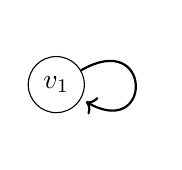
\begin{tikzpicture}[main node/.style={circle,fill=white!20,draw,font=\sffamily\normalsize\bfseries},scale=1]
        \node[main node, scale=1] (A) at (0,0) {$v_1$};
        \path[->, thick] (A) edge[shorten >= 2pt, distance=30, out=30, in=-30] (A);
      \end{tikzpicture}
    }

    \put (2.5,8.55) {\textbf{(b)}}
    \put (3,7) {
      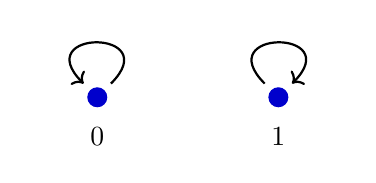
\begin{tikzpicture}
        \node at (1.2,-0.5) {$0$};
        \node at (3.5,-0.5) {$1$};
        \filldraw[blue!80!black] (1.2,0) circle (0.12);
        \filldraw[blue!80!black] (3.5,0) circle (0.12);
        \node (A) at (1.2,0) {};
        \node (B) at (3.5,0) {};
        \path[->, thick] (A) edge[shorten >= 2pt, shorten <= 2pt, distance=30, out=45, in=135] (A);
        \path[->, thick] (B) edge[shorten >= 2pt, shorten <= 2pt, distance=30, out=135, in=45] (B);
      \end{tikzpicture}
    }

    \put (8,8.55) {\textbf{(c)}}
    \put (9,7) {
      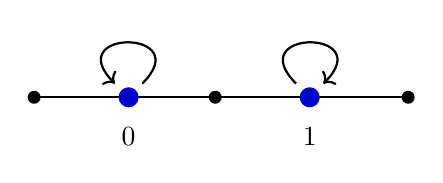
\begin{tikzpicture}
        \filldraw[black] (0,0) circle (0.075);
        \filldraw[black] (2.3,0) circle (0.075);
        \filldraw[black] (4.75,0) circle (0.075);
        \draw[-,thick] (0,0)--(4.75,0);
        \node at (1.2,-0.5) {$0$};
        \node at (3.5,-0.5) {$1$};
        \filldraw[blue!80!black] (1.2,0) circle (0.12);
        \filldraw[blue!80!black] (3.5,0) circle (0.12);
        \node (A) at (1.2,0) {};
        \node (B) at (3.5,0) {};
        \path[->, thick] (A) edge[shorten >= 2pt, shorten <= 2pt, distance=30, out=45, in=135] (A);
        \path[->, thick] (B) edge[shorten >= 2pt, shorten <= 2pt, distance=30, out=135, in=45] (B);
      \end{tikzpicture}
    }

    \put (0,5.5) {\textbf{(d)}}
    \put (0.5,4.5) {
      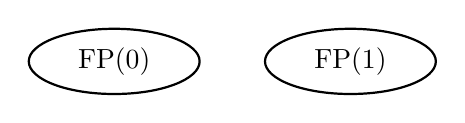
\begin{tikzpicture}
        \node[ellipse, draw, thick, text width=13mm, align = center] (10) at (1.5,0) {FP(1)};
        \node[ellipse, draw, thick, text width=13mm, align = center] (10) at (-1.5,0) {FP(0)};
      \end{tikzpicture}
    }

    \put (8,5.5) {\textbf{(e)}}
    \put (9,4.5) {
      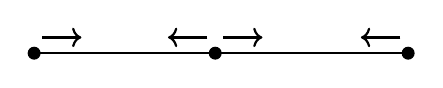
\begin{tikzpicture}
        \filldraw[black] (0,0) circle (0.075);
        \filldraw[black] (2.3,0) circle (0.075);
        \filldraw[black] (4.75,0) circle (0.075);
        \draw[-,thick] (0,0)--(4.75,0);
        \draw[->,thick] (0.1,0.2)--(0.6,0.2);
        \draw[->,thick] (2.2,0.2)--(1.7,0.2);
        \draw[->,thick] (2.4,0.2)--(2.9,0.2);
        \draw[->,thick] (4.65,0.2)--(4.15,0.2);
      \end{tikzpicture}
    }

    \put (0,2.5) {\textbf{(f)}}
    \put (1.0,1.5) {
      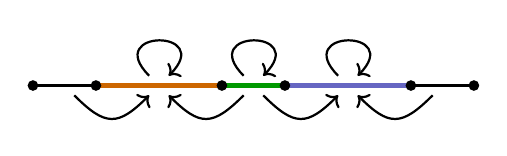
\begin{tikzpicture}[scale=0.8]
        \draw[-,thick] (0,0)--(7,0);
        \draw[-,black!20!orange,ultra thick] (1,0)--(3,0);
        \draw[-,black!40!green,ultra thick] (3,0)--(4,0);
        \draw[-,black!40!blue!60,ultra thick] (4,0)--(6,0);
        \filldraw[black] (0,0) circle (0.075);
        \filldraw[black] (1,0) circle (0.075);
        \filldraw[black] (3,0) circle (0.075);
        \filldraw[black] (4,0) circle (0.075);
        \filldraw[black] (6,0) circle (0.075);
        \filldraw[black] (7,0) circle (0.075);
        \node (A) at (0.5,0) {};
        \node (B) at (2.0,0) {};
        \node (C) at (3.5,0) {};
        \node (D) at (5.0,0) {};
        \node (E) at (6.5,0) {};
        \path[->, thick] (B) edge[distance=30, out=135, in=45] (B);
        \path[->, thick] (C) edge[distance=30, out=135, in=45] (C);
        \path[->, thick] (D) edge[distance=30, out=135, in=45] (D);
        \path[->, thick] (A) edge[distance=20, out=-45, in=-135] (B);
        \path[->, thick] (C) edge[distance=20, out=-135, in=-45] (B);
        \path[->, thick] (C) edge[distance=20, out=-45, in=-135] (D);
        \path[->, thick] (E) edge[distance=20, out=-135, in=-45] (D);
      \end{tikzpicture}
    }

    \put (8,2.5) {\textbf{(g)}}
    \put (9,0.5) {
      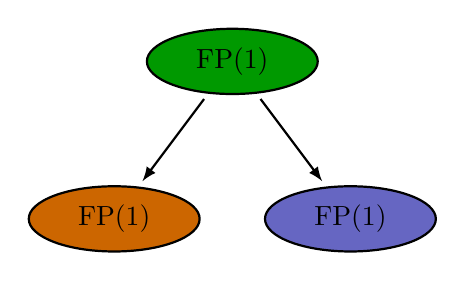
\begin{tikzpicture}
        \node[ellipse,draw,thick,black,fill=black!20!orange,text width=13mm,align=center] (10) at (-1.5,0) {FP(1)};
        \node[ellipse,draw,thick,black,fill=black!40!green,text width=13mm,align=center] (10) at (0,2) {FP(1)};
        \node[ellipse,draw,thick,black,fill=black!40!blue!60,text width=13mm,align=center] (10) at (1.5,0) {FP(1)};
        \draw[-latex, thick, shorten <= 17pt, shorten >= 17pt] (0,2)--(-1.5,0);
        \draw[-latex, thick, shorten <= 17pt, shorten >= 17pt] (0,2)--(1.5,0);
      \end{tikzpicture}
    }
  \end{picture}
  \caption{(a) A regulatory network \textbf{RN}. (b) The Boolean state transition graph. The blue dots correspond to the Boolean states $0$ and $1$. (c) The Boolean STG defined on a cubical cell complex $\cX$. The three black dots correspond to vertices of the cubical cell complex $\cX$. The black lines are edges of cubical cell complex. (d) The Boolean Morse graph given by the set of fixed points for Boolean state transition graph. (e) The DSGRN wall labeling on the cubical cell complex $\cX$. (f) The blowup cubical complex $\cX_b$ with the DSGRN STG mapping one-dimensional cells to one-dimensional cells. The green, blue, and orange edges are the cells in the complex $\cX_b$ corresponding to the nodes in the DSGRN Morse graph. (g) The DSGRN Morse graph of the DSGRN STG.}
  \label{fig:singleUp}
\end{figure}

In addition to the Boolean STG, Figure~\ref{fig:singleUp}(c) includes a one dimensional \textit{cubical complex} $\cX$ (see Definition~\ref{defn:Xcomplex}) that \textit{conceptually} shows the intended correspondence between the Boolean states and the domains of a continuous state space $[0, \infty)$ representing concentrations $x_1$ associated with node $v_1$. In particular, the Boolean state $0$ represents low concentrations of $x_1$ and the Boolean state $1$ represents high concentrations of $x_1$.

The cell complex $\cX$ consists of three zero-dimensional cells (the black dots): the leftmost that corresponds to $x_1 = 0$, the middle representing a threshold value of $x_1$ at which we consider that the concentration transitions from low to high, and the rightmost that corresponds to sufficiently large concentration;\footnote{We assume that the ODE system is dissipative. As a consequence there is an upper bound on the concentration of node $v_1$ at which the interesting dynamics occurs.  Sufficiently large concentration is any concentration above that.} and two one-dimensional cells connecting the zero-dimensional cells. The one dimensional cells correspond to the Boolean states $0$ and $1$ and represent the regions (intervals) in the continuous state space $[0, \infty)$ where the concentrations are low and high, respectively.

Figure~\ref{fig:singleUp}(d) shows the \textit{Boolean Morse graph} (see Definition~\ref{def:multi_Boolean_MG}) that characterizes reachability between maximal recurrent components of the Boolean STG. The two nodes in the Boolean Morse graph arise from recurrence imposed by the simple self edges at the two states of the Boolean STG. Furthermore, because the recurrent components consist of single states of the Boolean STG we label them as fixed points and indicate the corresponding states by labeling them $FP(0)$ and $FP(1)$, where $0$ and $1$ indicate the Boolean state corresponding to the fixed point. The Boolean Morse graph has no edges as there is no path in the Boolean STG from one recurrent component to another. The fact that the nodes are minimal nodes in the Morse graph (trivially true since the order relation on the Morse graph is trivial) is interpreted to mean that they represent stable dynamics.

The significance of the cubical cell complex $\cX$ is that it provides a stepping stone that allows one to systematically pass from the Boolean algebraic structures to the realm of topology and ODEs. This involves several steps. First, a wall labeling is defined on the walls of $\cX$ (see Definition~\ref{def:wall_labeling} and Theorem~\ref{thm:Boolen_wall_label}). The walls of $\cX$ consist of pairs $(\mu, \xi)$ where $\mu$ is $N$-dimensional cell (and edge in this example) and $\xi$ is an  $(N-1)$-dimensional face of $\mu$ (a vertex in this example). A wall labeling assigns a value of $-1$ or $+1$ to each wall of $\cX$ indicating whether the ``flow'' is moving towards or away from $\xi$. Figure~\ref{fig:singleUp}(e) shows the wall labeling, indicated by arrows, generated by $f_1^1$.

The wall labeling in Figure~\ref{fig:singleUp}(e) suggests that the middle vertex of $\cX$ represents unstable dynamics. Hence it suggests that nontrivial dynamics can occur on the lower dimensional cells of $\cX$. In order to capture this type of dynamics, a larger cell complex $\cX_b$, called the \textit{blowup cubical complex} (see \cite{rook_field:24}) is created. The blowup complex $\cX_b$ has the property that each cell in $\cX$ is represented by a top dimensional cell (in this case one-dimensional cell) in $\cX_b$.

Figure~\ref{fig:singleUp}(f) shows the blowup complex $\cX_b$ for the cell complex $\cX$ shown in Figure~\ref{fig:singleUp}(e). There are five one-dimensional cells in $\cX_b$ corresponding to the three zero-dimensional and the two one-dimensional cells of $\cX$. The DSGRN STG (see \cite{rook_field:24} and Remark~\ref{DSGRN_STG}) is given by the arrows between one-dimensional cells.

Figure~\ref{fig:singleUp}(g) shows the \textit{DSGRN Morse graph} (see Definition~\ref{def:DSGRN_MG}). The DSGRN Morse graph consists of three nodes that arise from the self edges at the one-dimensional cells colored (from left to right) in orange, green, and blue. Again, because the recurrent components consist of single states of the DSGRN STG we label them as fixed points $FP(1)$. For the DSGRN Morse graph we denote the nodes representing fixed points by $FP(k)$, where $k$ is the number of cells corresponding to the Morse node (see Definition~\ref{def:DSGRN_MG}).  The arrows from the green cell to the orange and blue cells gives rise to the ordering of green to blue and orange shown in the DSGRN Morse graph. The minimality of the blue and orange nodes is interpreted to mean that they represent stable objects.

\begin{rem}
  There are significant differences between the Boolean Morse graph and the DSGRN Morse graph. If one adopts the perspective that ODEs provide an appropriate model for the dynamics associated with the regulatory network  of Figure~\ref{fig:singleUp}(a), then these difference have important implications and demonstrate shortcomings of purely Boolean modeling. If we assume that $[0,\infty)$ is an appropriate phase space for the dynamics, then it is impossible to have two attractors without a separatrix. The DSGRN Morse graph identifies this separatrix via the green node while the Boolean Morse graph does not.
\end{rem}

We repeat this analysis by considering a one node network with a repressing edge as shown in Figure~\ref{fig:singleDown}(a). We again consider $f_1^1 = {\bf I}$. However the repressing edge introduces a change of variables $\beta$ (see \eqref{eq:beta}) that transform $f_1^1$ into a decreasing monotone Boolean functions $g_1^1 \colon \B\to \B$. In this example $g_1^1 = \neg {\bf I}$, i.e., $g_1^1(0) = 1$ and $g_1^1(1) = 0$. The Boolean function $g_1^1$ is used to produce the the Boolean STG represented by Figures~\ref{fig:singleDown}(b) and \ref{fig:singleDown}(c). The state transition graph has two nodes $0$ and $1$ and the fact that $g_1^1(0) = 1$ and $g_1^1(1) = 0$ produces asynchronous update directed edges going back and forth between both of them.

Figure~\ref{fig:singleDown}(c) shows the \textit{cubical complex} $\cX$, and Figure~\ref{fig:singleDown}(d) shows the Boolean Morse graph consisting of a single node. Since the associated recurrent component contains both states of the Boolean STG we denote it by $FC$ (full cycle) suggesting that the dynamics performs a cycle. As before, the fact that the node is a minimal node of the Morse graph is interpreted to mean that the $FC$ represents stable dynamics. Figure~\ref{fig:singleDown}(e) shows the wall labeling generated by $f_1^1$ and Figure~\ref{fig:singleDown}(f) shows the blowup complex $\cX_b$ for the cubical complex $\cX$ shown in Figure~\ref{fig:singleDown}(c). The Boolean function $f_1^1$ is used to compute the DSGRN STG which is given by the arrows between one-dimensional cells in Figure~\ref{fig:singleDown}(f). Figure~\ref{fig:singleDown}(g) shows the DSGRN Morse graph that consists of a single node labeled $FP(1)$.

\begin{figure}[htp!]
  \centering
  \setlength{\unitlength}{1cm}
  \begin{picture}(15.5,4) %width / height

    \put (0,3.55) {\textbf{(a)}}
    \put (0.5,2) {
      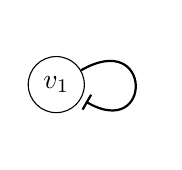
\begin{tikzpicture}[main node/.style={circle,fill=white!20,draw,font=\sffamily\normalsize\bfseries},scale=1]
        \node[main node, scale=1] (A) at (0,0) {$v_1$};
        \path[-|, thick] (A) edge[shorten >= 2pt, distance=30, out=30, in=-30] (A);
      \end{tikzpicture}
    }

    \put (2.3,3.55) {\textbf{(b)}}
    \put (2.8,2) {
      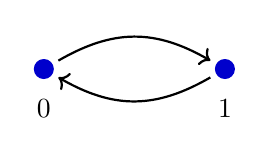
\begin{tikzpicture}
        \node at (1.2,-0.5) {$0$};
        \node at (3.5,-0.5) {$1$};
        \filldraw[blue!80!black] (1.2,0) circle (0.12);
        \filldraw[blue!80!black] (3.5,0) circle (0.12);
        \node (A) at (1.2,0) {};
        \node (B) at (3.5,0) {};
        \path[->, thick] (A) edge[shorten >= 2pt, shorten <= 2pt, distance=25, out=30, in=150] (B);
        \path[->, thick] (B) edge[shorten >= 2pt, shorten <= 2pt, distance=25, out=210, in=-30] (A);
      \end{tikzpicture}
    }

    \put (6,3.55) {\textbf{(c)}}
    \put (6.5,2) {
      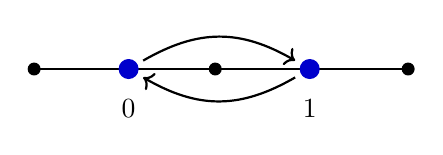
\begin{tikzpicture}
        \filldraw[black] (0,0) circle (0.075);
        \filldraw[black] (2.3,0) circle (0.075);
        \filldraw[black] (4.75,0) circle (0.075);
        \draw[-,thick] (0,0)--(4.75,0);
        \node at (1.2,-0.5) {$0$};
        \node at (3.5,-0.5) {$1$};
        \filldraw[blue!80!black] (1.2,0) circle (0.12);
        \filldraw[blue!80!black] (3.5,0) circle (0.12);
        \node (A) at (1.2,0) {};
        \node (B) at (3.5,0) {};
        \path[->, thick] (A) edge[shorten >= 2pt, shorten <= 2pt, distance=25, out=30, in=150] (B);
        \path[->, thick] (B) edge[shorten >= 2pt, shorten <= 2pt, distance=25, out=210, in=-30] (A);
      \end{tikzpicture}
    }

    \put (12.7,3.55) {\textbf{(d)}}
    \put (13.2,2.3) {
      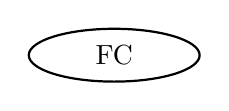
\begin{tikzpicture}
        \node[ellipse,draw,thick,text width=13mm,align=center] (10) at (1.5,0) {FC};
      \end{tikzpicture}
    }

    \put (0,1) {\textbf{(e)}}
    \put (0.5,0.5) {
      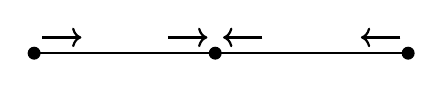
\begin{tikzpicture}
        \filldraw[black] (0,0) circle (0.075);
        \filldraw[black] (2.3,0) circle (0.075);
        \filldraw[black] (4.75,0) circle (0.075);
        \draw[-,thick] (0,0)--(4.75,0);
        \draw[->,thick] (0.1,0.2)--(0.6,0.2);
        \draw[->,thick] (1.7,0.2)--(2.2,0.2);
        \draw[->,thick] (2.9,0.2)--(2.4,0.2);
        \draw[->,thick] (4.65,0.2)--(4.15,0.2);
      \end{tikzpicture}
    }

    \put (6.0,1) {\textbf{(f)}}
    \put (6.5,0) {
      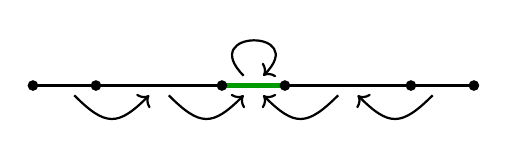
\begin{tikzpicture}[scale=0.8]
        \draw[-,thick] (0,0)--(7,0);
        \draw[-,black!40!green,ultra thick] (3,0)--(4,0);
        \filldraw[black] (0,0) circle (0.075);
        \filldraw[black] (1,0) circle (0.075);
        \filldraw[black] (3,0) circle (0.075);
        \filldraw[black] (4,0) circle (0.075);
        \filldraw[black] (6,0) circle (0.075);
        \filldraw[black] (7,0) circle (0.075);
        \node (A) at (0.5,0) {};
        \node (B) at (2.0,0) {};
        \node (C) at (3.5,0) {};
        \node (D) at (5.0,0) {};
        \node (E) at (6.5,0) {};
        \path[->, thick] (C) edge[distance=30, out=135, in=45] (C);
        \path[->, thick] (A) edge[distance=20, out=-45, in=-135] (B);
        \path[->, thick] (B) edge[distance=20, out=-45, in=-135] (C);
        \path[->, thick] (E) edge[distance=20, out=-135, in=-45] (D);
        \path[->, thick] (D) edge[distance=20, out=-135, in=-45] (C);
      \end{tikzpicture}
    }

    \put (12.7,1) {\textbf{(g)}}
    \put (13.2,0.2) {
      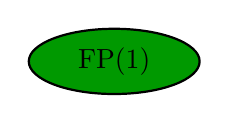
\begin{tikzpicture}
        \node[ellipse,draw,thick,black,fill=black!40!green,text width=13mm,align=center] (10) at (0,0) {FP(1)};
      \end{tikzpicture}
    }
  \end{picture}
  \caption{(a) A regulatory network \textbf{RN}. (b) The Boolean state transition graph. The blue dots correspond to the Boolean states $0$ and $1$. (c) The Boolean STG defined on a cubical cell complex $\cX$. The three black dots correspond to vertices of the cubical cell complex $\cX$. The black lines are edges of cubical cell complex. (d) The Boolean Morse Graph for the Boolean STG consists of one node identified as a full cycle ($FC$). (e) The DSGRN wall labeling on the cubical cell complex $\cX$. (f) The blowup cubical complex $\cX_b$ with the DSGRN STG mapping one-dimensional cells to one-dimensional cells. The green edge is the cell in the complex $\cX_b$ corresponding to the node in the DSGRN Morse graph. (g) The DSGRN Morse graph of the DSGRN STG.}
  \label{fig:singleDown}
\end{figure}

\begin{rem}
  Adopting the perspective that ODEs provide an appropriate model for the dynamics associated with the regulatory network of Figure~\ref{fig:singleDown}(a), the difference in labeling between the Boolean Morse graph and the DSGRN Morse graph is significant. The Boolean Morse graph suggest the existence of stable oscillatory dynamics. This is impossible if the phase space is $[0, \infty)$. The DSGRN Morse graph suggests the existence of a stable fixed point which is consistent with ODE dynamics on $[0, \infty)$.
\end{rem}

%%%%%%%%%%%%%%%%%%%%%%%%%%%%%%%%%%%%%%%%%%%%%%%%%%%%%%%%%%%%%%%%%%%%%%%%%%%%%%%%
\subsection{The toggle switch}
\label{subsec:TS}

We study the toggle-switch~\cite{toggle}, a well-studied two node network, to begin to demonstrate that the dynamics of multi-node networks can be organized using products based on single nodes. The network, shown in Figure~\ref{fig:toggle}(a), consists of two nodes with mutually repressive edges.

\begin{figure}[htp!]
  \centering %%% Param 27
  \setlength{\unitlength}{1cm}
  \begin{picture}(13.3,10) %width / height

    \put (0,9) {\textbf{(a)}}
    \put (1.0,6.5) {
      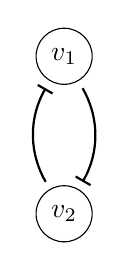
\begin{tikzpicture}[main node/.style={circle,fill=white!20,draw,font=\sffamily\normalsize\bfseries},scale=1]
        \node[main node, scale=1] (A) at (1,1) {$v_1$};
        \node[main node, scale=1] (B) at (1,-1) {$v_2$};
        \path[->,>=angle 90,thick]
        (A) edge[-|,bend left, shorten <= 3pt, shorten >= 3pt] (B)
        (B) edge[-|,bend left, shorten <= 3pt, shorten >= 3pt] (A);
      \end{tikzpicture}
    }

    \put (5.5,9) {\textbf{(b)}}
    \put (6.5,6) {
      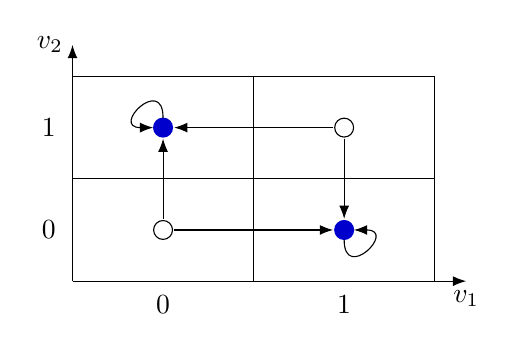
\begin{tikzpicture}
        \draw[->,-Latex] (0,0)--(5,0) node[pos=1, below] {$v_1$};
        \draw[->,-Latex] (0,0)--(0,3) node[pos=1, left] {$v_2$};
        \draw[-] (2.3,0)--(2.3,2.6);
        \draw[-] (4.6,0)--(4.6,2.6);
        \draw[-] (0,1.3)--(4.6,1.3);
        \draw[-] (0,2.6)--(4.6,2.6);
        \draw (1.15,0.65) circle (0.12);
        \filldraw[blue!80!black] (3.45,0.65) circle (0.12);
        \filldraw[blue!80!black] (1.15,1.95) circle (0.12);
        \draw (3.45,1.95) circle (0.12);
        \node (A) at (1.15,1.95) {};
        \node (B) at (3.45,0.65) {};
        \draw (A)[->, -Latex] to [out=90,in=180,looseness=8] (A);
        \draw (B)[->, -Latex] to [out=270,in=0,looseness=8] (B);
        \draw[->, -Latex, shorten <= 4pt, shorten >= 4pt] (1.15,0.65)--(1.15,1.95);
        \draw [->, -Latex, shorten <= 4pt, shorten >= 4pt] (3.45,1.95)--(3.45,0.65);
        \draw [->, -Latex, shorten <= 4pt, shorten >= 4pt] (1.15,0.65)--(3.45,0.65);
        \draw [->, -Latex, shorten <= 4pt, shorten >= 4pt] (3.45,1.95)--(1.15,1.95);
        \node (n) at (1.15,-0.3) {$0$};
        \node (n) at (3.45,-0.3) {$1$};
        \node (n) at (-0.3,0.65) {$0$};
        \node (n) at (-0.3,1.95) {$1$};
      \end{tikzpicture}
    }

    \put (0,5) {\textbf{(c)}}
    \put (0.5,0) {
      \includegraphics[width=0.33\textwidth]{figures/example_3_morse_sets.pdf}
    }

    \put (7,5) {\textbf{(d)}}
    \put (8,4) {
      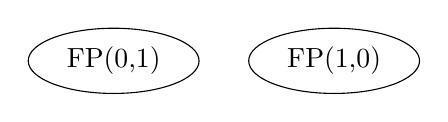
\begin{tikzpicture}
        \node[ellipse, draw, text width=13mm, align=center] (10) at (1.4,0) {FP(1,0)};
        \node[ellipse, draw, text width=13mm, align=center] (10) at (-1.4,0) {FP(0,1)};
      \end{tikzpicture}
    }

    \put (7,3.0) {\textbf{(e)}}
    \put (6.5,-0.5) {
      \includegraphics[width=0.3\textwidth]{figures/example_3_morse_graph.pdf}
    }
  \end{picture}
  \caption{(a) A regulatory network \textbf{RN} (the toggle switch). (b) The Boolean STG defined on a two-dimensional cubical complex $\cX$. (c) The blowup cubical complex $\cX_b$ and the DSGRN STG. (d) Set of fixed points for Boolean state transition graph. (e) The Morse graph computed by DSGRN for the STG in (c).}
  \label{fig:toggle}
\end{figure}

As in the examples of Section~\ref{subsec:snn} each node can assume one of the two states in $\B = \setof{ 0,1 }$. The two edges in the network indicate that a Boolean model for this network consist of two increasing MBFs $f_1^2$ and $f_2^1$ representing the regulations of node $1$ on node $2$ and of node $2$ on node $1$, respectively. We consider $f_1^2 = f_2^1 = {\bf I}$ as the MBFs representing the DSGRN parameter node for the network. As before, the repressing edges introduces a change of variables $\beta$, given by \eqref{eq:beta}, that transform $f_1^2$ and $f_2^1$ into decreasing MBFs $g_1^2, g_2^1$. In this example $g_1^2 = g_2^1 = \neg {\bf I}$. The Boolean functions $g_i^j$ are used to produce the the Boolean STG represented in Figure~\ref{fig:toggle}(b). The Boolean STG has four nodes $\setof{(0,0),(0,1),(1,0),(1,1)}$. The asynchronous update edges are shown in Figure~\ref{fig:toggle}(b).

Given that there are two nodes, $1$ and $2$, the associated concentrations $x_1$ and $x_2$ lie in the phase space $[0,\infty)^2$. Thus, as is shown in Figure~\ref{fig:toggle}(b), we make use of a two-dimensional cubical complex $\cX$ to conceptually relate the Boolean states with domains in $[0,\infty)^2$. Figure~\ref{fig:toggle}(d) shows the Boolean Morse graph. The nodes are the two fixed points that arise from the self-edges at states $(0,1)$ and $(1,0)$ and are denoted by $FP(0,1)$ and $FP(1,0)$, respectively. The are both minimal with respect to the associated partial order given by the Morse graph (the trivial partial order) and hence represent stable states.

Figure~\ref{fig:toggle} (c)shows the blowup cubical complex $\cX_b$ where each zero, one, or two-dimensional cell of the cubical complex $\cX$ in Figure~\ref{fig:toggle}(b)  is represented by a two dimensional cell. The arrows indicate the DSGRN STG and the black dots indicate self edges. Figure~\ref{fig:singleUp}(e) shows the DSGRN Morse graph, which consists of three nodes that arise from the self edges at the two-dimensional cells colored (from upper left to lower right) in orange, green, and blue. Again, because the recurrent components consist of single states of the DSGRN STG we label them as fixed points $FP$. The arrows from the green cell to the orange and blue cells gives rise to the ordering of green to blue and orange shown in the DSGRN Morse graph. The minimality of the blue and orange nodes is interpreted to mean that they represent stable objects. We index the nodes of the Morse graph as nodes $0$, $1$, and $2$ and label each node as $FP(k)$, where $k$ is the number of cells in the complex $\cX_b$ corresponding to the Morse node (in this example $k = 1$ for all nodes).

\begin{rem}
  The  differences between the Boolean Morse graph and the DSGRN Morse graph for the toggle switch are the same as those of the single-node network with an activating edge. Again, from the perspective of ODEs, if we assume that $[0,\infty)^2$ is an appropriate phase space for the dynamics, then it is impossible to have two attractors without a separatrix as is suggested by the Boolean Morse graph. However, the DSGRN Morse graph identifies this separatrix via the green node.
\end{rem}

%%%%%%%%%%%%%%%%%%%%%%%%%%%%%%%%%%%%%%%%%%%%%%%%%%%%%%%%%%%%%%%%%%%%%%%%%%%%%%%%
\subsection{Multilevel discrete models}
\label{sec:multilevel_models}

The key change from a Boolean model to a multilevel model is the assignment of a distinct ``threshold'' to each edge in a $RN$ (see Section~\ref{sec:multilevel_RN}). Each threshold is then associated with a choice of a MBF, permitting different downstream effects of a source node to a target node. For intuition, a single threshold of node $v_1$ in Figure~\ref{fig:network_boolean}(a) controls the impact of $v_1$ on both of its outgoing edges, $v_1 \to v_1$ and $v_1 \dashv v_2$, as demonstrated in the Boolean STG shown in Figures~\ref{fig:network_boolean}(b) and \ref{fig:network_boolean}(c). We then ``unfold'' the threshold for $v_1$ into two thresholds, one for each out edge with a choice of an order, as shown in Figures~\ref{fig:multi1}(c) and \ref{fig:multi2}(c). We initially consider an unfolding in which the MBF is identical for the two thresholds (Figure~\ref{fig:multi1}), and then proceed to a more general example where the two functions are not identical (Figure~\ref{fig:multi2}).

To describe the relationship between the set of  monotone Boolean functions and multilevel discrete models we need to consider networks with nodes that have more than one target. A particularly simple example is shown in Figure~\ref{fig:network_boolean}(a). This is a two-node network where node $v_1$ has two targets (itself and node $v_2$) and two inputs, while node $v_2$ has one target (node $v_1$) and one input (also node $v_1$).

\begin{figure}[htp!]
  \centering
  \setlength{\unitlength}{1cm}
  \begin{picture}(13.7,4.6) %width / height

    \put (0,4.1) {\textbf{(a)}}
    \put (0,0.4) {
      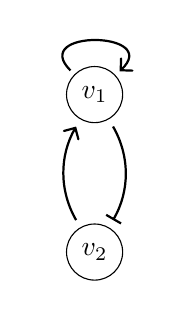
\begin{tikzpicture}[main node/.style={circle,fill=white!20,draw,font=\sffamily\normalsize\bfseries},scale=1]
        \node[main node, scale=1] (A) at (1,1) {$v_1$};
        \node[main node, scale=1] (B) at (1,-1) {$v_2$};
        \path[->,>=angle 90,thick]
        (A) edge[out= 135,in= 43,looseness=4,shorten <= 2pt, shorten >= 2pt] (A)
        (A) edge[-|,bend left, shorten <= 3pt, shorten >= 3pt] (B)
        (B) edge[->,bend left, shorten <= 3pt, shorten >= 3pt] (A);
      \end{tikzpicture}
    }

    \put (2.3,4.1) {\textbf{(b)}}
    \put (2.3,0) {
      \begin{tikzpicture}
        \draw[->, -Latex] (0,0)--(4.75,0) node[pos=1, below] {$v_1$};
        \draw[-, dashed] (2.3,0)--(2.3,3);
        \draw[-, dashed] (0,1.5)--(4.75,1.5);
        \draw[->, -Latex] (0,0)--(0,3) node[pos=1, left] {$v_2$};
        \filldraw[blue!80!black] (1.2,2.2) circle (0.12);
        \draw (1.2,0.8) circle (0.12);
        \draw (3.5,2.2) circle (0.12);
        \draw (3.5,0.8) circle (0.12);
        \node (A) at (1.2,2.2) {};
        \draw[->, -Latex] (A) to [out=90,in=180,looseness=8] (A);
        \draw[->, -Latex] (1.2,0.91)--(1.2,2.1);
        \draw[->, -Latex] (3.4,0.8)--(1.3,0.8);
        \draw[->, -Latex] (3.5,2.1)--(3.5,0.91);
        % \draw[->, -Latex] (3.38,2.2)--(1.32,2.2);
        \node (n) at (-0.4,2.2) {$1$};
        \node (n) at (-0.4, 0.8) {$0$};
        \node (n) at (1.2, -0.4) {$0$};
        \node (n) at (3.5, -0.4) {$1$};
      \end{tikzpicture}
    }

    \put (8.1,4.1) {\textbf{(c)}}
    \put (8.1,0) {
      \begin{tikzpicture}
        \draw[->, -Latex] (0,0)--(4.75,0) node[pos=1, below] {$v_1$};
        \draw[-,dashed] (2.3,0)--(2.3,3);
        \draw[-,dashed] (0,1.5)--(4.75,1.5);
        \draw[->, -Latex] (0,0)--(0,3) node[pos=1, left] {$v_2$};
        \filldraw[blue!80!black] (3.5,0.8) circle (0.12);
        \draw (1.2,0.8) circle (0.12);
        \draw (3.5,2.2) circle (0.12);
        \draw (1.2,2.2) circle (0.12);
        \node (A) at (3.5,0.8) {};
        \draw[->, -Latex] (A) to [out=270,in=0,looseness=8] (A);
        \draw[->, -Latex] (1.2,.91)--(1.2,2.1);
        \draw[->, -Latex] (3.5,2.1)--(3.5,0.91);
        \draw[->, -Latex] (1.32,2.2)--(3.38,2.2);
        \node (n) at (-0.4,2.2) {$1$};
        \node (n) at (-0.4, 0.8) {$0$};
        \node (n) at (1.2, -0.4) {$0$};
        \node (n) at (3.5, -0.4) {$1$};
      \end{tikzpicture}
    }
  \end{picture}
  \caption{(a) A regulatory network $RN$. (b) The Boolean STG represented on a cubical complex $\cX$ with $f_1 = \wedge$. (c) The Boolean STG represented on a cubical complex $\cX$ with $f_1= \vee$.}
  \label{fig:network_boolean}
\end{figure}

We first consider the dynamics (STG) of the network in Figure~\ref{fig:network_boolean}(a) generated by a Boolean model $f \colon \B^2 \to \B^2$, with $f = (f_1, f_2)$. Because $v_1$ has two inputs we have that $f_1 \colon \B^2 \to \B$. The fact that the edges from $v_1$ and $v_2$ to $v_1$ are activating implies that $f_1$ is an increasing MBF. We consider two choices for node $v_1$: $f_1 = \wedge$ and $f_1 = \vee$. Because node $v_2$ has one input and one target its structure is the same as that of nodes discussed in Sections~\ref{subsec:snn} and \ref{subsec:TS}. The fact that there is a single input implies that $f_2 \colon \B \to \B$ and the fact that the edge from node $v_1$ to node $v_2$ is repressing implies that $f_2$ is a decreasing MBF. We consider the case $f_2 = \neg {\bf I}$.

For each choice of $f_1$ we compute the Boolean STG given by Definition~\ref{def:Boolean_update}. When the choice of MBF for node $v_1$ is $f_1 = \wedge$, then the resulting Boolean STG is the one in Figure~\ref{fig:multi1}(b). When $f_1 = \vee$ the resulting Boolean STG is the one in Figure~\ref{fig:multi1}(c).

We now ``unfold'' the threshold for $v_1$ into two thresholds, that is, we consider one MBF for each edge in the network. Hence we have the following MBFs (see Definition~\ref{def:fi}): $f_1^1$ and $f_1^2$, corresponding to the out edges of node $v_1$, and $f_2^1$ corresponding to the out edge of node $v_2$. Recall that a DSGRN logic parameter consists of increasing MBFs (see Definition~\ref{def:fi} and Remark~\ref{rem:increasing_MBFs}) hence the functions $f_i^j$ are increasing MBFs. We first consider the case where $f_1^1 = f_1^2$ and take $f_1^1 = f_1^2 = \wedge$ and $f_2^1 = {\bf I}$. Since now we have tow out edges for node $v_1$ and an increasing MBF corresponding to each edge, we need to decide the order in which the MBFs $f_1^1$ and $f_1^2$ are ``turned on''. This is done via an order parameter (see Definition~\ref{defn:order_parameter}). For this example we consider the order parameter $\theta$ satisfying $\theta_1(1) < \theta_1(2)$. These choices give a parameter node $p = (f, \theta) \in \PG$. The parameter $p$ defines the multilevel Boolean STG (see Defintion~\ref{def:Boolean_update}) on the state space $\cD = \setof{(0,0),(1,0),(2,0), (0,1), (1,1), (2,1)}$ shown in Figure~\ref{fig:multi1}(a). Figure~\ref{fig:multi1}(b) shows the multi Boolean Morse graph that consists of a single node. Since the associated recurrent component consists of the single state $(0, 1)$ of the Boolean STG we denote it by $FP(0,1)$. Figure~\ref{fig:multi1}(b) shows the blowup cubical complex $\cX_b$ and the DSGRN STG. The same fixed point is identified by DSGRN as shown in the DSGRN Morse graph in Figure~\ref{fig:multi1}(c).

\begin{figure}[htp!]
  \centering
  \setlength{\unitlength}{1cm}
  \begin{picture}(12.5,9.8) %width / height

    \put (0,9.5) {\textbf{(a)}}
    \put (0.7,5.6) {
      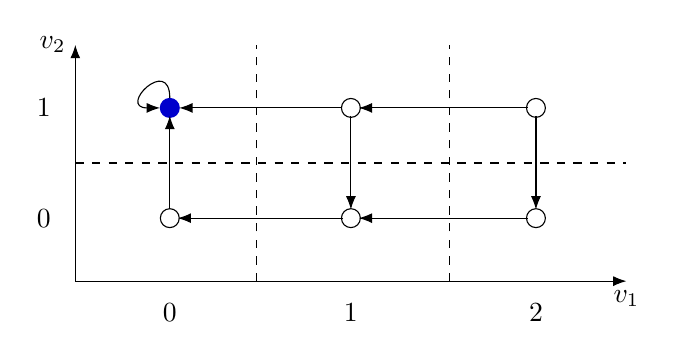
\begin{tikzpicture}
        \draw[->, -Latex] (0,0)--(7,0) node[pos=1, below] {$v_1$};
        \draw[-,dashed] (2.3,0)--(2.3,3);
        \draw[-,dashed] (4.75,0)--(4.75,3);
        \draw[-,dashed] (0,1.5)--(7,1.5);
        \draw[->, -Latex] (0,0)--(0,3) node[pos=1, left] {$v_2$};
        \filldraw[blue!80!black] (1.2,2.2) circle (0.12);
        \draw (1.2,0.8) circle (0.12);
        \draw (5.85,2.2) circle (0.12);
        \draw (5.85,0.8) circle (0.12);
        \draw (3.5,2.2) circle (0.12);
        \draw (3.5,0.8) circle (0.12);
        \node (A) at (1.2,2.2) {};
        \draw[->, -Latex] (A) to [out=90,in=180,looseness=8] (A);
        \draw[->, -Latex] (1.2,0.91)--(1.2,2.1);
        \draw[->, -Latex] (3.4,0.8)--(1.3,0.8);
        \draw[->, -Latex] (3.5,2.1)--(3.5,0.91);
        \draw[->, -Latex] (5.85,2.1)--(5.85,0.91);
        \draw[->, -Latex] (5.749,2.2)--(3.6,2.2);
        \draw[->, -Latex] (3.38,2.2)--(1.32,2.2);
        \draw[->, -Latex] (5.749,0.8)--(3.6,0.8);
        \node (n) at (-0.4,2.2) {$1$};
        \node (n) at (-0.4, .8) {$0$};
        \node (n) at (1.2, -0.4) {$0$};
        \node (n) at (3.5, -0.4) {$1$};
        \node (n) at (5.85, -0.4) {$2$};
      \end{tikzpicture}
    }

    \put (9,9.5) {\textbf{(b)}}
    \put (9.8,7.5) {
      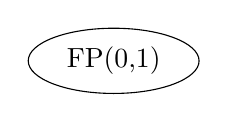
\begin{tikzpicture}
        \node[ellipse, draw, text width=13mm, align = center] (11) at (0,0) {FP(0,1)};
      \end{tikzpicture}
    }

    \put (0,5.2) {\textbf{(c)}}
    \put (0.7,-0.4) {
      \includegraphics[width=0.5\textwidth]{figures/example_4_morse_sets.pdf}
    }

    \put (9.2,5.2) {\textbf{(d)}}
    \put (9.2,2.5) {
      \includegraphics[width=0.25\textwidth]{figures/example_4_morse_graph.pdf}
    }
  \end{picture}
  \caption{(a) The ``unfolded'' multilevel Boolean STG with for $f_1^1 = f_1^2 = \wedge$ and $\theta_1(1) < \theta_1(2)$ corresponding to the Boolean STG in Figure~\ref{fig:network_boolean}(b). (b) Multi Boolean STG with a single fixed point. (c) The DSGRN STG also detects the same fixed point. (d) The DSGRN Morse graph is isomorphic to the multi Boolean Morse graph.}
  \label{fig:multi1}
\end{figure}

\begin{rem}
  Based on this example, it may seem that choosing the same MBF for both edges does not fully utilize the freedom of the larger phase space to produce more dynamics. This is actually false, as we will show that threshold order can non-trivially impact dynamics (Section~\ref{sec:orders}).
\end{rem}

We now modify the Boolean representation so that the targets of $v_1$ can be triggered by different Boolean functions. We consider the same network as in Figure~\ref{fig:multi1}(a) and choose $f_1^1= \vee$ and $f_1^2 = \wedge$ to examine. In this scenario, there is no clear comparison to any Boolean STG, since in the Boolean setting there is a single Boolean function $f_1$ associated to node $v_1$ and we must choose either $f_1 = \wedge$ or $f_1 = \vee$. For the former choice, see Figure~\ref{fig:network_boolean}(b), and for the latter choice, see Figure~\ref{fig:network_boolean}(c).

The choice $f_1^1= \vee$ and $f_1^2 = \wedge$ substantially changes the state transition graph from both of the Boolean STGs in Figures~\ref{fig:network_boolean}(b) and (c), as well as from the multilevel STG in Figure~\ref{fig:multi2}(a). The multilevel STG now produces the existence of a cyclic strongly connected component denoted by $FC$ (Full Cycle) shown in Figure~\ref{fig:multi2}(b).

The DSGRN STG in Figure~\ref{fig:multi2}(c) shows that the existence of both cyclic behavior and a fixed point. However the DSGRN Morse (Figure~\ref{fig:multi2}(d)) identifies the cyclic behavior as possibly representing trivial dynamics (see Definition~\ref{def:DSGRN_MG}) and hence labels it as $T(8)$ since it is composed of $8$ cells. The reason the Morse graph in Figure~\ref{fig:multi2}(d) labels the cycling Morse node as trivial is that the state transition graph in Figure~\ref{fig:multi2}(c) does not provide enough information to decide whether trajectories of the continuous system just pass through the orange region and converge to blue fixed point, or there is a periodic orbit within the orange.

As we briefly explain in Section~\ref{sec:Morse_graph}, DSGRN software computes an algebraic-topological invariant called the \textit{Conley index} for each Morse node. If this invariant is non-trivial, then the domain(s) corresponding to the Morse node contain an invariant set of the continuous process. If the invariant is trivial, more detailed information about the dynamics is needed to reach a conclusion.

\begin{figure}[htp!]
  \centering
  \setlength{\unitlength}{1cm}
  \begin{picture}(12.5,9.8) %width / height

    \put (0,9.5) {\textbf{(a)}}
    \put (0.7,5.6) {
      \begin{tikzpicture}
        \draw[->, -Latex] (0,0)--(7,0) node[pos=1, below] {$v_1$};
        \draw[-,dashed] (2.3,0)--(2.3,3);
        \draw[-,dashed] (4.75,0)--(4.75,3);
        \draw[-,dashed] (0,1.5)--(7,1.5);
        \draw[->, -Latex] (0,0)--(0,3) node[pos=1, left] {$v_2$};
        \draw (1.2,2.2) circle (0.12);
        \draw (1.2,0.8) circle (0.12);
        \draw (5.85,2.2) circle (0.12);
        \draw (5.85,0.8) circle (0.12);
        \draw (3.5,2.2) circle (0.12);
        \draw (3.5,0.8) circle (0.12);
        \node (A) at (1.2,2.2) {};
        \draw[->, -Latex] (A) to (3.4,2.2);
        \draw[->, -Latex] (1.2,0.91)--(1.2,2.1);
        \draw[->, -Latex] (3.5,0.91)--(3.5,2.1);
        \draw[->, -Latex] (5.85,2.1)--(5.85,0.91);
        \draw[->, -Latex] (5.749,0.8)--(3.6,0.8);
        \draw[->, -Latex] (3.6,2.2)--(5.749,2.2);
        \node (n) at (-0.4,2.2) {$1$};
        \node (n) at (-0.4, 0.8) {$0$};
        \node (n) at (1.2, -0.4) {$0$};
        \node (n) at (3.5, -0.4) {$1$};
        \node (n) at (5.85, -0.4) {$2$};
      \end{tikzpicture}
    }

    \put (9,9.5) {\textbf{(b)}}
    \put (9.8,7.5) {
      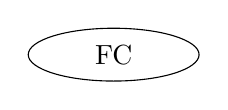
\begin{tikzpicture}
        \node[ellipse, draw, text width=13mm, align = center] (10) at (2.4,0) {FC};
      \end{tikzpicture}
    }

    \put (0,5.2) {\textbf{(c)}}
    \put (0.7,-0.4) {
      \includegraphics[width=0.5\textwidth]{figures/example_5_new_morse_sets.pdf}
    }

    \put (9.2,5.2) {\textbf{(d)}}
    \put (9.2,1.0) {
      \includegraphics[width=0.2\textwidth]{figures/example_5_new_morse_graph.pdf}
    }
  \end{picture}
  \caption{(a) The multilevel Boolean STG. (b) The multi Boolean STG identifies a full cycle (FC) through the states $(1,0)$, $(1,1)$, $(2,1)$, and $(2,0)$. (c) The DSGRN STG detects existence of both cyclic behavior and a fixed point. (d) The DSGRN Morse graph for the dynamics computed by DSGRN is compatible with ODE dynamics.}
  \label{fig:multi2}
\end{figure}

%%%%%%%%%%%%%%%%%%%%%%%%%%%%%%%%%%%%%%%%%%%%%%%%%%%%%%%%%%%%%%%%%%%%%%%%%%%%%%%%
\subsection{Threshold order affects network dynamics}
\label{sec:orders}

It is perhaps not surprising that having more states in the state transition graph of the multi-level discrete map than in the Boolean map and the freedom of having separate Boolean functions associated to different edges produces richer dynamics. This is illustrated by comparing Figure~\ref{fig:network_boolean} which shows dynamics of monotone Boolean functions with Figures~\ref{fig:multi1} and \ref{fig:multi2} showing a more general scenario.

We now consider the network in Figure~\ref{fig:22network}(a) and compare the Boolean and the DSGRN state transition graphs when we change the order parameters. For the Boolean STG we consider the following MBFs: $h_1(b_1, b_2) = b_1 \wedge b_2$ and $h_2(b_1, b_2) = \neg b_1 \wedge b_2$. The state transition graph for this Boolean system is in  Figure~\ref{fig:22network}(b).

\begin{figure}[htp!]
  \centering
  \setlength{\unitlength}{1cm}
  \begin{picture}(8.5,4.6) %width / height

    \put (0,4.1) {\textbf{(a)}}
    \put (0.3,0) {
      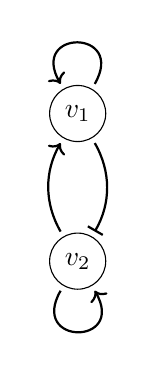
\begin{tikzpicture}
        [main node/.style={circle,fill=white!20,draw},scale=2.5]
        \node[main node] (1) at (0, 0.75) {$v_1$};
        \node[main node] (2) at (0, 0) {$v_2$};
        \path[thick]
        (1) edge[-|, shorten <= 2pt, shorten >= 2pt, bend left] (2)
        (1) edge[->, loop right, distance=10pt, shorten <= 2pt, shorten >= 2pt, thick, in=120, out=60] (1)
        (2) edge[->, shorten <= 2pt, shorten >= 2pt, bend left] (1)
        (2) edge[->, loop left, distance=10pt, shorten <= 2pt, shorten >= 2pt, thick, in=300, out=240] (2);
      \end{tikzpicture}
    }

    \put (2.5,4.1) {\textbf{(b)}}
    \put (2.7,0) {
      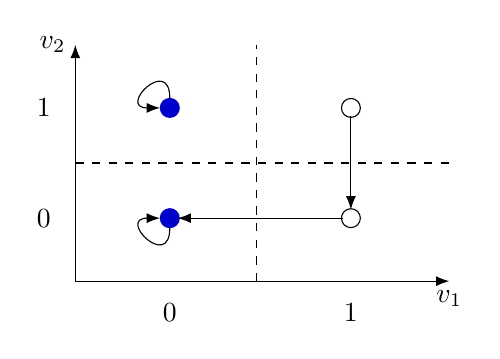
\begin{tikzpicture}
        \draw[->, -Latex] (0,0)--(4.75,0) node[pos=1, below] {$v_1$};
        \draw[-, dashed] (2.3,0)--(2.3,3);
        \draw[-, dashed] (0,1.5)--(4.75,1.5);
        \draw[->, -Latex] (0,0)--(0,3) node[pos=1, left] {$v_2$};
        \filldraw[blue!80!black] (1.2,2.2) circle (0.12);
        \filldraw[blue!80!black] (1.2,0.8) circle (0.12);
        \draw (3.5,2.2) circle (0.12);
        \draw (3.5,0.8) circle (0.12);
        \node (A) at (1.2,2.2) {};
        \node (B) at (1.2,0.8) {};
        \draw[->, -Latex] (A) to [out=90,in=180,looseness=8] (A);
        \draw[->, -Latex] (B) to [out=270,in=180,looseness=8] (B);
        \draw[->, -Latex] (3.4,0.8)--(1.3,0.8);
        \draw[->, -Latex] (3.5,2.1)--(3.5,0.91);
        \node (n) at (-0.4,2.2) {$1$};
        \node (n) at (-0.4, 0.8) {$0$};
        \node (n) at (1.2, -0.4) {$0$};
        \node (n) at (3.5, -0.4) {$1$};
      \end{tikzpicture}
    }
  \end{picture}
  \caption{(a) Regulatory network $RN$. (b) The Boolean STG represented on a cubical complex $\cX$ with $h_1$ and $h_2$.}
  \label{fig:22network}
\end{figure}

To compute the DSGRN state transition graph we apply the change of variables $\beta$ given by \eqref{eq:beta} which gives $f_1 = f_2 = \wedge$ and consider the logic parameter $f = ((f_1, f_1), (f_2, f_2))$.

Since both nodes in the network in Figure~\ref{fig:22network}(a) have two targets, the order parameter for node $v_1$ is given by $\{ \theta_1(1), \theta_1(2) \}$ and for node $v_2$ by $\{ \theta_2(1), \theta_2(2) \}$. There are two ways to order each of these sets and hence there are four different set of parameters with the same logic parameter $f$ and different order parameter $\theta$. We consider all four possible order parameters:
\begin{equation}
  \label{order:4p}
  \begin{aligned}
    (\theta_1(1) < \theta_1(2), \theta_2(2) < \theta_2(1)), \\
    (\theta_1(2) < \theta_1(1), \theta_2(2) < \theta_2(1)), \\
    (\theta_1(1) < \theta_1(2), \theta_2(1) < \theta_2(2)), \\
    (\theta_1(2) < \theta_1(1), \theta_2(1) < \theta_2(2)).
  \end{aligned}
\end{equation}

The DSGRN state transition graphs and corresponding Morse graphs for the four different order parameters given in (\ref{order:4p} are shown in Figure~\ref{fig:order_flow}. We note that the DSGRN STG produces different dynamics for different order parameters and that these dynamics are all refinements of the Boolean dynamics generated by the STG in Figure~\ref{fig:22network}(b). The blue are orange fixed points in Figure~\ref{fig:order_flow} correspond to the two fixed points in Figure~\ref{fig:22network}(b).

  \begin{figure}
    \begin{tabular}{cccc}
      \includegraphics[width=0.25\textwidth]{figures/example_6_order_1_morse_sets.pdf} &
      \includegraphics[width=0.22\textwidth]{figures/example_6_order_1_morse_graph.pdf} &
      \includegraphics[width=0.25\textwidth]{figures/example_6_order_2_morse_sets.pdf} &
      \includegraphics[width=0.2\textwidth]{figures/example_6_order_2_morse_graph.pdf} \\
      ($a_1$) & ($a_2$) & ($b_1$) & ($b_2$) \\
      \includegraphics[width=0.25\textwidth]{figures/example_6_order_3_morse_sets.pdf} &
      \includegraphics[width=0.2\textwidth]{figures/example_6_order_3_morse_graph.pdf} &
      \includegraphics[width=0.25\textwidth]{figures/example_6_order_4_morse_sets.pdf} &
      \includegraphics[width=0.2\textwidth]{figures/example_6_order_4_morse_graph.pdf} \\
      ($c_1$) & ($c_2$) & ($d_1$) & ($d_2$)
    \end{tabular}
    \caption{DSGRN state transition graphs and corresponding Morse graphs for the four different order parameters given in (\ref{order:4p}).}
    \label{fig:order_flow}
  \end{figure}
  \Bernardo{alternative: can add threshold ordering to label}
  \begin{figure}
    \centering
    \begin{tabular}{cc}
      \begin{subfigure}[b]{0.50\textwidth}
        \centering
        \includegraphics[width=0.48\linewidth]{figures/example_6_order_1_morse_sets.pdf}
        \includegraphics[width=0.48\linewidth]{figures/example_6_order_1_morse_graph.pdf}
        \caption{Order 1}
      \end{subfigure} &
      \begin{subfigure}[b]{0.50\textwidth}
        \centering
        \includegraphics[width=0.48\linewidth]{figures/example_6_order_2_morse_sets.pdf}
        \includegraphics[width=0.48\linewidth]{figures/example_6_order_2_morse_graph.pdf}
        \caption{Order 2}
      \end{subfigure} \\
      \begin{subfigure}[b]{0.50\textwidth}
        \centering
        \includegraphics[width=0.48\linewidth]{figures/example_6_order_3_morse_sets.pdf}
        \includegraphics[width=0.48\linewidth]{figures/example_6_order_3_morse_graph.pdf}
        \caption{Order 3}
      \end{subfigure} &
      \begin{subfigure}[b]{0.50\textwidth}
        \centering
        \includegraphics[width=0.48\linewidth]{figures/example_6_order_4_morse_sets.pdf}
        \includegraphics[width=0.48\linewidth]{figures/example_6_order_4_morse_graph.pdf}
        \caption{Order 4}
      \end{subfigure}
    \end{tabular}
    \caption{DSGRN state transition graphs and corresponding Morse graphs for the four different order parameters given in (\ref{order:4p}).}
    \label{fig:order_flow}
  \end{figure}

  %%%%%%%%%%%%%%%%%%%%%%%%%%%%%%%%%%%%%%%%%%%%%%%%%%%%%%%%%%%%%%%%%%%%%%%%%%%%%%%%
  \subsection{The DSGRN parameter graph}

  The collection of all DSGRN parameters for a given network is organized in the DSGRN parameter graph $\PG$ (see Section~\ref{sec:PG}). The nodes of $\PG$ consist of all possible increasing monotone Boolean functions and all order parameters for the given network.

  We denote by ${\mathbf 0}$ the constant Boolean function $0$ (i.e., ${\mathbf 0}(0) = {\mathbf 0}(1) = 0$) and by ${\mathbf 1}$ the constant Boolean function $1$ (i.e., ${\mathbf 1}(0) = {\mathbf 1}(1) = 1$). The DSGRN parameter graph for the regulatory networks in Figures~\ref{fig:singleUp}(a) and \ref{fig:singleDown}(a) are the same and is shown in Figure~\ref{fig:PG_single_toggle}(a). The reason both of those networks have the same parameter graph is because the edges signs are encoded by the network via the edge sign function $\delta$ and not by the parameters in the parameter graph (see Remark~\ref{rem:increasing_MBFs}). The parameter graph for the network in Figure~\ref{fig:toggle} is shown in Figure~\ref{fig:PG_single_toggle}(b). Notice that the order parameter is not present in the parameter graphs in Figure~\ref{fig:PG_single_toggle}. That is because the corresponding network have a single out edge per node and hence the order parameter is trivial. The order parameter is non-trivial for networks having nodes with at least two edges as in Figure~\ref{fig:22network}(a). The parameter graph for the network in Figure~\ref{fig:22network}(a) has $120$ nodes (see Section~\ref{sec:more_examples}) for additional discussions on parameter graphs.

  \begin{figure}[htp!]
    \centering
    \setlength{\unitlength}{1cm}
    \begin{picture}(9.5,4.7) %width / height

      \put (0,4.1) {\textbf{(a)}}
      \put (0.3,1.7) {
        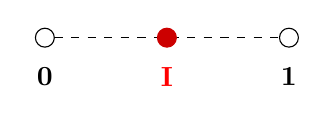
\begin{tikzpicture}
          \draw[-,dashed] (1.62,2.0)--(4.5,2.0);
          \draw (1.5,2.0) circle (0.12);
          \filldraw[red!80!black] (3.05,2.0) circle (0.12);
          \draw (4.6,2.0) circle (0.12);
          \node (0x) at (1.5,1.5) {$\mathbf{0}$};
          \node (Ix) at (3.05,1.5) {${\color{red} \mathbf{I}}$};
          \node (1x) at (4.6,1.5) {$\mathbf{1}$};
          % \draw[-] (1.7,1.5)--(2.9,1.5);
          % \draw[-] (3.2,1.5)--(4.4,1.5);
        \end{tikzpicture}
      }

      \put (4.8,4.1) {\textbf{(b)}}
      \put (5.2,0.0) {
        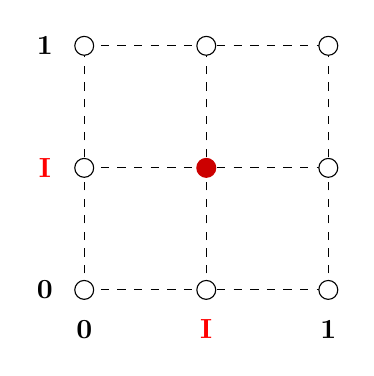
\begin{tikzpicture}
          % Horizontal
          \draw[-,dashed] (1.5,1.5)--(4.6,1.5);
          \draw[-,dashed] (1.5,3.05)--(4.6,3.05);
          \draw[-,dashed] (1.5,4.6)--(4.6,4.6);
          % Vertical
          \draw[-,dashed] (1.5,1.5)--(1.5,4.6);
          \draw[-,dashed] (3.05,1.5)--(3.05,4.6);
          \draw[-,dashed] (4.6,1.5)--(4.6,4.6);
          % Circles
          \filldraw[fill=white, draw=black] (1.5,1.5) circle (0.12);
          \filldraw[fill=white, draw=black] (3.05,1.5) circle (0.12);
          \filldraw[fill=white, draw=black] (4.6,1.5) circle (0.12);
          \filldraw[fill=white, draw=black] (1.5,3.05) circle (0.12);
          \filldraw[red!80!black] (3.05,3.05) circle (0.12);
          \filldraw[fill=white, draw=black] (4.6,3.05) circle (0.12);
          \filldraw[fill=white, draw=black] (1.5,4.6) circle (0.12);
          \filldraw[fill=white, draw=black] (3.05,4.6) circle (0.12);
          \filldraw[fill=white, draw=black] (4.6,4.6) circle (0.12);
          % Labels
          \node (0x) at (1.5,1.0) {$\mathbf{0}$};
          \node (Ix) at (3.05,1.0) {${\color{red} \mathbf{I}}$};
          \node (1x) at (4.6,1.0) {$\mathbf{1}$};
          % \draw[-] (1.7,1.0)--(2.9,1.0);
          % \draw[-] (3.2,1.0)--(4.4,1.0);
          \node (0y) at (1.0,1.5) {$\mathbf{0}$};
          \node (Iy) at (1.0,3.05) {${\color{red} \mathbf{I}}$};
          \node (1y) at (1.0,4.6) {$\mathbf{1}$};
          % \draw[-] (1.0,1.7)--(1.0,2.8);
          % \draw[-] (1.0,3.3)--(1.0,4.35);
        \end{tikzpicture}
      }
    \end{picture}
    \caption{(a) Parameter graph for the networks in Figures~\ref{fig:singleUp}(a) and \ref{fig:singleDown}(a). (b) Parameter graph for the network in Figure~\ref{fig:toggle}(a).}
    \label{fig:PG_single_toggle}
  \end{figure}

  %%%%%%%%%%%%%%%%%%%%%%%%%%%%%%%%%%%%%%%%%%%%%%%%%%%%%%%%%%%%%%%%%%%%%%%%%%%%%%%%
  \subsection{Embedding of Boolean functions into the parameter graph}

  In Figures~\ref{boolean_flow}(a) and (c) we show the state transition graphs for two MBF models $f = (f_1, f_2)$ and $\tilde{f} = (\tilde{f}_1, \tilde{f}_2)$ for the network in Figure~\ref{fig:toggle}, where $f_1(b_1, b_2) = \tilde{f}_1(b_1, b_2) = b_1 \wedge b_2$, $f_2(b_1, b_2) = \neg b_1 \wedge b_2$, and $\tilde{f}_2(b_1, b_2) = \neg b_1 \vee b_2$. Note that $f$ and $\tilde{f}$ differ only in the second component where the essential Boolean function $f_2(b_1, b_2) = \neg b_1 \wedge b_2$ is replaced by the another essential Boolean function $\tilde{f}_2(b_1, b_2) = \neg b_1 \vee b_2$. Since $f_2$ and $\tilde{f}_2$ are the only two essential monotone Boolean functions with two inputs for this network, they are the closest neighbors within the set of essential monotone Boolean functions. However, the state transition graphs in Figures~\ref{boolean_flow}(a) and (c) are very different. In particular, in the states $(0, 1)$ and $(1, 0)$ the functions have the same value, but in the other two states $(0, 0)$ and $(1, 1)$ the values of the components of $f_2$ and $\tilde{f}_2$ change. This means that there is no obvious continuity between the STG generated by $f$ and STG generated by $\tilde{f}$. However, if we also consider non-essential MBFs this transition is more gradual. There are two non-essential MBFs whose values are between $f_2$ and $\tilde{f}_2$. These are the functions $h_2 (b_1, b_2) = \neg b_1$ which does not depend on the second input and the function $\tilde{h}_2 (b_1, b_2) = b_2$ which does not depend on the first input. In Figure~\ref{boolean_flow}(b) we show the STG of the MBF model $h = (f_1, h_2)$. The difference between the STG of $f$ and the STG of $h$ is in the state $(1, 0)$ while the difference between the STG of $\tilde{f}$ and the STG of $h$ is in the state $(0, 1)$. Therefore we can interpret $h$ as providing an interpolation  between $f$ and $\tilde{f}$.

  \begin{figure}[htp!]
    \centering
    \setlength{\unitlength}{1cm}
    \begin{picture}(16.2,4.6) %width / height

      \put (-0.2,4.1) {\textbf{(a)}}
      \put (-0.2,0) {
        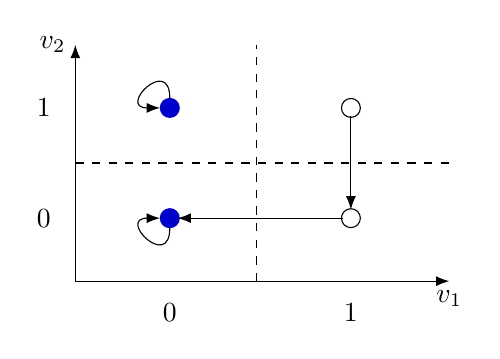
\begin{tikzpicture}
          \draw[->, -Latex] (0,0)--(4.75,0) node[pos=1, below] {$v_1$};
          \draw[-, dashed] (2.3,0)--(2.3,3);
          \draw[-, dashed] (0,1.5)--(4.75,1.5);
          \draw[->, -Latex] (0,0)--(0,3) node[pos=1, left] {$v_2$};
          \filldraw[blue!80!black] (1.2,2.2) circle (0.12);
          \filldraw[blue!80!black] (1.2,0.8) circle (0.12);
          \draw (3.5,2.2) circle (0.12);
          \draw (3.5,0.8) circle (0.12);
          \node (A) at (1.2,2.2) {};
          \node (B) at (1.2,0.8) {};
          \draw[->, -Latex] (A) to [out=90,in=180,looseness=8] (A);
          \draw[->, -Latex] (B) to [out=270,in=180,looseness=8] (B);
          \draw[->, -Latex] (3.4,0.8)--(1.3,0.8);
          \draw[->, -Latex] (3.5,2.1)--(3.5,0.91);
          \node (n) at (-0.4,2.2) {$1$};
          \node (n) at (-0.4, 0.8) {$0$};
          \node (n) at (1.2, -0.4) {$0$};
          \node (n) at (3.5, -0.4) {$1$};
        \end{tikzpicture}
      }

      \put (5.3,4.1) {\textbf{(b)}}
      \put (5.3,0) {
        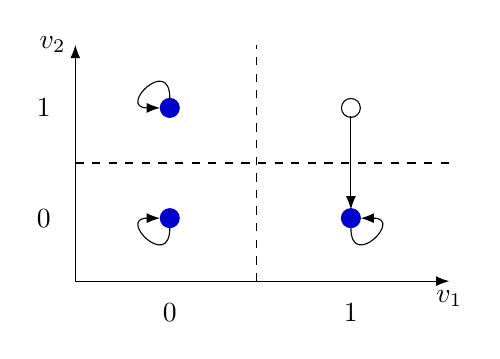
\begin{tikzpicture}
          \draw[->, -Latex] (0,0)--(4.75,0) node[pos=1, below] {$v_1$};
          \draw[-, dashed] (2.3,0)--(2.3,3);
          \draw[-, dashed] (0,1.5)--(4.75,1.5);
          \draw[->, -Latex] (0,0)--(0,3) node[pos=1, left] {$v_2$};
          \filldraw[blue!80!black] (1.2,2.2) circle (0.12);
          \filldraw[blue!80!black] (1.2,0.8) circle (0.12);
          \filldraw[blue!80!black] (3.5,0.8) circle (0.12);
          \draw (3.5,2.2) circle (0.12);
          \node (A) at (1.2,2.2) {};
          \node (B) at (1.2,0.8) {};
          \node (C) at (3.5,0.8) {};
          \draw[->, -Latex] (A) to [out=90,in=180,looseness=8] (A);
          \draw[->, -Latex] (B) to [out=270,in=180,looseness=8] (B);
          \draw[->, -Latex] (C) to [out=270,in=0,looseness=8] (C);
          \draw[->, -Latex] (3.5,2.1)--(3.5,0.91);
          \node (n) at (-0.4,2.2) {$1$};
          \node (n) at (-0.4, 0.8) {$0$};
          \node (n) at (1.2, -0.4) {$0$};
          \node (n) at (3.5, -0.4) {$1$};
        \end{tikzpicture}
      }

      \put (10.7,4.1) {\textbf{(c)}}
      \put (10.7,0) {
        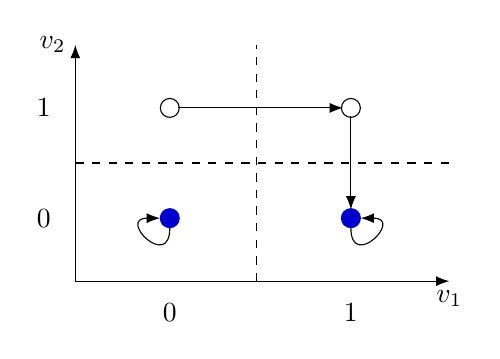
\begin{tikzpicture}
          \draw[->, -Latex] (0,0)--(4.75,0) node[pos=1, below] {$v_1$};
          \draw[-, dashed] (2.3,0)--(2.3,3);
          \draw[-, dashed] (0,1.5)--(4.75,1.5);
          \draw[->, -Latex] (0,0)--(0,3) node[pos=1, left] {$v_2$};
          \filldraw[blue!80!black] (1.2,0.8) circle (0.12);
          \filldraw[blue!80!black] (3.5,0.8) circle (0.12);
          \draw (1.2,2.2) circle (0.12);
          \draw (3.5,2.2) circle (0.12);
          \node (B) at (1.2,0.8) {};
          \node (C) at (3.5,0.8) {};
          \draw[->, -Latex] (B) to [out=270,in=180,looseness=8] (B);
          \draw[->, -Latex] (C) to [out=270,in=0,looseness=8] (C);
          \draw[->, -Latex] (1.3,2.2)--(3.4,2.2);
          \draw[->, -Latex] (3.5,2.1)--(3.5,0.91);
          \node (n) at (-0.4,2.2) {$1$};
          \node (n) at (-0.4, 0.8) {$0$};
          \node (n) at (1.2, -0.4) {$0$};
          \node (n) at (3.5, -0.4) {$1$};
        \end{tikzpicture}
      }
    \end{picture}
    \caption{(a) The Boolean STG of $f$. (b) The Boolean STG of $h$. (c) The Boolean STG of $\tilde{f}$.}
    \label{boolean_flow}
  \end{figure}

  %%%%%%%%%%%%%%%%%%%%%%%%%%%%%%%%%%%%%%%%%%%%%%%%%%%%%%%%%%%%%%%%%%%%%%%%%%%%%%%%
  \section{Mathematical background and results}
  \label{sec:math}

  In this section we present the necessary mathematical background and results. We denote by $\bbB := \{ 0, 1 \}$ the Boolean lattice with $0 < 1$. Depending on the context, the value $0$ represents \textsf{FALSE} or the state \textsf{OFF} and value $1$ represents \textsf{TRUE} or the state \textsf{ON}. We denote the negation of $b \in \bbB$ by $\neg b$, that is, $\neg 0 = 1$ and $\neg 1 = 0$.

  %%%%%%%%%%%%%%%%%%%%%%%%%%%%%%%%%%%%%%%%%%%%%%%%%%%%%%%%%%%%%%%%%%%%%%%%%%%%%%%%
  \subsection{Monotone Boolean functions}

  \begin{defn}
    \label{def:RN}
    A \textit{regulatory network} $RN = (V, E, \delta)$ is a directed graph with nodes $V = \{ 1, 2, \ldots, N \}$, directed edges $E$, and an edge sign function $\delta \colon E \to \{-1, 1\}$. We denote an edge from node $i$ to node $j$ by $(i, j)$. The edge $(i, j)$ is \textit{activating} if $\delta(i, j) = 1$ and \textit{repressing} if $\delta(i, j) = -1$. Graphically, we denote an edge $(i, j)$ without indicating its sign by
    $i \multimap j$, and we denote an activating edge by $i \to j$ and a repressing edge by $i \dashv j$. The \textit{sources} and \textit{targets} of a node $i$ are given by
    \[
      \Sources(i):= \setdef{k \in V}{(k, i) \in E} \ \text{ and } \ \Targets(i):= \setdef{j \in V}{(i, j) \in E},
    \]
    respectively.
  \end{defn}

  For the sake of clarity of exposition, in a slight abuse of notation, we often assign labels $\{ v_1, v_2, \ldots, v_N \}$ to the nodes $V$ and denote a node $i$ and and edge $i \multimap j$ by $v_i$ and $v_i \multimap v_j$, respectively. In this paper we use both notations interchangeably.

  \begin{defn}
    \label{def:lattice}
    Let $\bbB := \{ 0, 1 \}$ be a Boolean lattice. A \emph{Boolean function} is a function $f \colon \bbB^n \to \bbB$. A vector valued function $f \colon \bbB^n \to \bbB^n$, $f = (f_1, \ldots, f_n)$, is called a \emph{Boolean model}.
  \end{defn}

  \begin{defn}
    A Boolean function $f \colon \bbB^n \to \bbB$ is \emph{increasing  with respect to input $j$} if for any $b = (b_1, \ldots, b_n) \in \bbB^n$
    \[
      f(b_1, \ldots, b_{j-1}, 0, b_{j+1}, \ldots, b_n) \leq f(b_1 \ldots, b_{j-1}, 1, b_{j+1}, \ldots, b_n).
    \]
    It is \emph{strictly increasing  with respect to input $j$} if there is at least one $b \in \bbB^n$ for which the inequality is strict.

    A Boolean function $f \colon \bbB^n \to \bbB$ is \emph{decreasing  with respect to input $j$} if for any $b = (b_1, \ldots, b_n) \in \bbB^n$
    \[
      f(b_1, \ldots, b_{j-1}, 0, b_{j+1}, \ldots, b_n) \geq f(b_1, \ldots, b_{j-1}, 1, b_{j+1}, \ldots, b_n).
    \]
    It is \emph{strictly decreasing with respect to input $j$} if there is at least one $b \in \bbB^n$ for which the inequality is strict.
  \end{defn}

  \begin{defn}
    \label{defn:MBF}
    A Boolean function $f \colon \bbB^n \to \bbB$ is \emph{monotone} if it is increasing or decreasing with respect to each input $j = 1, \ldots, n$. In this case $f$ is called a \emph{monotone Boolean function} (MBF).
  \end{defn}

  A special type of monotone Boolean function is increasing with respect to all of its inputs. In this case an equivalent formulation is the following.

  \begin{defn}
    \label{defn:MBF_increasing}
    Let $(\bbB^n, \preceq)$ be a Boolean lattice with partial order induced component-wise by $0 < 1$. A Boolean function $f \colon \bbB^n \to \bbB$ is \emph{monotone increasing} if for all $z, w \in \bbB^n$
    \[
      z \preceq w \qquad \implies \qquad f(z) \leq f(w).
    \]
  \end{defn}

  \begin{defn}
    A Boolean model $f \colon \bbB^n \to \bbB^n$ is \emph{monotone} if $f_i$ is monotone for every $i = 1, \ldots, n$.
  \end{defn}

  \begin{defn}
    \label{def:regulatory_network}
    Given a monotone Boolean model $f \colon \bbB^n \to \bbB^n$, its associated \emph{influence network} is the regulatory network $RN(f) = (V, E, \delta)$ defined by
    \begin{enumerate}[(i)]
      \item $V = \{1, \ldots, n \}$,
      \item $(i, j) \in E$ if and only if $f_j$ is not constant with respect to the input $i$,
      \item $\delta \colon E \to \{1, -1\}$ is given by
        \[
          \delta(i, j) =
          \begin{cases}
            \;\;\, 1  & \text{if } f_j \text{ is strictly increasing with respect to input } i \\
            -1 & \text{if } f_j \text{ is strictly decreasing with respect to input } i
          \end{cases}
        \]
    \end{enumerate}
  \end{defn}

  \begin{defn}
    Let $RN = (V, E, \delta)$ be a regulatory network with $V = \{ 1, 2, \ldots, N \}$. A monotone Boolean model $f \colon \bbB^N \to \bbB^N$ is a \emph{monotone Boolean model} for $RN$ if its influence network is a signed subgraph of $RN$, that is, if it is a subgraph and the sign functions agree on the common edges. If $RN(f)=RN$, then we say that $f$ is an \emph{essential monotone Boolean model} for $RN$.
  \end{defn}

  Note that any monotone Boolean function $f \colon \bbB^n \to \bbB$ can be written in terms of a monotone increasing Boolean function
  $h \colon \bbB^n \to \bbB$ as a composition
  \begin{equation}
    \label{eq:beta}
    f(b) = h(\beta(b)),
  \end{equation}
  where the component $\beta_i \colon \bbB^n \to \bbB$ of the map $\beta \colon \bbB^n \to \bbB^n$ is defined by
  \[
    \beta_i(b) =
    \begin{cases}
      \;\;\, b_i, & \text{if } f \text{ is increasing with respect to input } i \\
      \neg b_i,   & \text{if } f \text{ is decreasing with respect to input } i
    \end{cases}
  \]

  It follows that any monotone Boolean model $f = (f_1, \ldots, f_n)$ for a regulatory network $RN$ corresponds to an increasing  monotone Boolean models $h = (h_1, \ldots, h_n)$ where the change of variables $\beta$ is given by the network (see \eqref{def:B} and the discussion that follows).

  Therefore from now on we describe the structure of increasing monotone Boolean functions. When considering Boolean models of networks with negative edges we construct the change of variable function $\beta$ in \eqref{eq:beta}.

  The set of monotone increasing Boolean functions with $k$ inputs is large and its size is the $k$-th Dedekind number \cite{Kleitman1969}, which is known for $k \leq 9$. Since we can represent any monotone Boolean function $f$ in terms of an increasing monotone Boolean function $h$ as in \eqref{eq:beta}, the Dedekind number is also the number of monotone Boolean functions with any fixed monotonicity with respect to its inputs.

  %%%%%%%%%%%%%%%%%%%%%%%%%%%%%%%%%%%%%%%%%%%%%%%%%%%%%%%%%%%%%%%%%%%%%%%%%%%%%%%%
  \subsection{Boolean models}

  Given a regulatory network $RN$ and a monotone Boolean model $f \colon \bbB^N \to \bbB^N$ we define a multivalued map $\cF \colon \bbB^N \rightrightarrows \bbB^N$, called the \textit{asynchronous update multivalued map}, which is used to compute the \emph{Boolean dynamics} of the network.

  \begin{defn}
    \label{def:Boolean_update}
    The \textit{asynchronous update multivalued map} is the map $\cF \colon \bbB^N \rightrightarrows \bbB^N$ generated by $f$ and defined by:
    \begin{itemize}
      \item If $f(b) = b$, then $\cF(b) = \{ b \}$.
      \item If $f(b) \neq b$, then $\ol{b} \in \cF(b)$ if and only if there exists $i \in V$ and $\eta \in \{-1, 1\}$ such that $\eta f_i(b) > \eta b_i$ and
        \[
          \ol{b}_i = b_i + \eta, \quad \ol{b}_j = b_j \mbox{ for } j\neq i.
        \]
    \end{itemize}
    The multi-valued map $\cF$ on $\bbB^N$ is also called the \textit{Boolean state transition graph}.
  \end{defn}

  %%%%%%%%%%%%%%%%%%%%%%%%%%%%%%%%%%%%%%%%%%%%%%%%%%%%%%%%%%%%%%%%%%%%%%%%%%%%%%%%
  \subsection{Finite multilevel models compatible with $RN$}
  \label{sec:multilevel_RN}

  Given a regulatory network $RN = (V, E, \delta)$ with $V = \{ 1, 2, \ldots, N \}$, we and others have proposed \cite{Ironi2011,Cummins16,Gedeon20,Richard2006} a larger class of finite multilevel models compatible with the network structure. For each node $j$ we consider all possible ways in which the collection of its input edges $\{ (i, j) \in E \ | \ i \in \Sources(j) \}$ can ``turn on'' a subset of its output edges $\{ (j, k) \in E \ | \ k \in \Targets(j) \}$.

  The precise notion of an edge being turned on is presented in Definition~\ref{def:turn_on}. Recall that we consider only increasing monotone Boolean models for the network. Informally, if an activating edge $v_i \to v_j$ is turned on it presents the input $1$ (\textsf{ON}) to node $v_j$ and hence it is sending an activating signal to $v_j$. If a repressing edge $v_i \dashv v_j$ is turned on it presents the input $0$ (\textsf{OFF}) to node $v_j$ and hence it is sending a repressing signal to $v_j$. If an edge $v_i \multimap v_j$ is not turned on it presents the opposite input to $v_j$.

  Note that in a traditional Boolean model~\cite{glass:kaufman:73,glass:kaufman:73,Thomas95,Thomas1973} each node $v_i$ has associated to it a single Boolean variable which can be in one of the two states $0$ or $1$, which is determined by a Boolean function of its inputs. The state $1$ then turns on all of the output edges of $v_i$ and the state $0$ does not turn on any of the output edges of $v_i$. Hence the output edges of a node $v_i$ are either all turned on or none of them are turned on.

  If we want a discrete network model that represents a continuous process, the pattern of the subsets of the output edges of a node $v_i$ that are turned on must be representable as a response to varying levels of expression of the continuous variable $x_i$, which may represent concentration, associated to node $v_i$. Hence we need a model where the edge $v_i \multimap v_j$ is turned on by the node $v_i$ only when the value of $x_i$ passes a certain level, or threshold, associated with the edge $v_i \multimap v_j$. Therefore we need a discrete network model where, unlike in a traditional Boolean model, a particular input $b \in \bbB^N$ to a node $v_i$ may turn on only some, but not all, of the edges $v_i \multimap v_j$ with $v_j \in \Targets(v_i)$.

  In order to describe such a discrete model we need a notion of a ``discrete threshold'' associated to an edge, corresponding to the continuous threshold associated with the continuous variable $x_i$. In principle, there can be more than one discrete threshold associated to an edge $v_i \multimap v_j$. However, the simplest model satisfying these conditions has a single threshold for each edge. The crucial constraint imposed by this view of the process of turning on some, but not all, the edges is that the discrete thresholds at which individual edges are turned on must be ordered. Hence our notion of a ``discrete threshold'' is simply an ordering of the output edges of each node $v_i$ and is formalized as an \emph{order parameter} defined below.

  We next describe the set of \emph{DSGRN parameters} associated with the regulatory network $RN$ \cite{E2,duncan3}, each of which uniquely defines a finite multilevel discrete model. We follow the exposition in~\cite{E2}.

  We first define an order parameter for a node $i$ of a regulatory network. Given a node $i \in V$ let $m_i:= | \Targets(i) |$ denote the number of out-edges of $i$.

  \begin{defn}
    \label{defn:order_parameter}
    An \emph{order parameter} for a node $i \in V$ is an ordering  of the set $\Targets(i)$, that is, it is a bijection $\theta_i \colon \Targets(i) \to \{1, \ldots, m_i \}$.
  \end{defn}

  Note that an order parameter is just a total ordering of the out-edges of $i$. This total order represents the order in which the out edges $\{ (i, j) \ | \ j \in \Targets(i) \}$ of $i$ are turned on.

  The set of order parameters for $i$ is denoted by $\Theta(i)$. The set of all order parameters is given by $\Theta := \prod_{i=1}^{N} \Theta(i)$.

  Next, we define the \textit{logic parameters} for the regulatory network $RN = (V,E,\delta)$.

  \begin{defn}
    \label{def:fi}
    A \textit{logic parameter} for a node $i$ of the regulatory network $RN = (V,E,\delta)$ is a vector valued function
    \begin{equation}
      \label{eq:logical}
      f_i \colon \bbB^{|\Sources(i)|} \to \bbB^{|\Targets(i)|}, \quad f_i = (f_i^1, \ldots, f_i^{m_i}),
    \end{equation}
    whose components $f_i^k \colon \bbB^{|\Sources(i)|} \to \bbB$ are increasing monotone Boolean functions satisfying the \textit{ordering conditions}
    \begin{equation}
      \label{eq:ordering condition}
      f_i^1(b) \succeq \cdots \succeq f_i^{m_i}(b)
    \end{equation}
    for all $b \in \bbB^{|\Sources(i)|}$.
  \end{defn}

  The functions $f_i^j$ are used in conjunction with an order parameter $\theta_i$ and their purpose is to describe when an input $b$ turns on the out-edges of $v_i$. More precisely, the function $f_i^{\theta_i(j)}$ describes when an input $b$ turns on the edge $v_i \multimap v_j$ associated with $\theta_i(j)$ as follows:
  \begin{itemize}
    \item If $f_i^{\theta_i(j)}(b) = 1$, then $b$ turns on the edge $v_i \multimap v_j$;
    \item If $f_i^{\theta_i(j)}(b) = 0$, then $b$ does not turn on the edge $v_i \multimap v_j$.
  \end{itemize}

  The set of all logic parameters for node $i$ is denoted $\cL(i)$. The set of all logic parameters is $\cL := \prod_{i=1}^{N} \cL(v_i)$.

  The set of parameters for node $i$ is $\cP(i) := \cL(i) \times \Theta(i)$. The set of parameters for the regulatory network is given by the product $\cP := \prod_{i=1}^{N} \cP(i)$. In a slight abuse of notation we identify the set of parameter $\cP$ with the the product of logic and order parameters $\cP = \cL \times \Theta$ and denote a parameter $p \in \cP$ by $p = (f, \theta)$.

  We call the set of parameters $\cP$ the set of \textit{DSGRN multilevel Boolean parameters}. However we often refer to them just as \emph{DSGRN parameters} or simply as \textit{parameters}.

  In the next section we endow the set of parameters $\cP$ with a graph structure by defining an adjacency relation between the elements of $\cP$.

  %%%%%%%%%%%%%%%%%%%%%%%%%%%%%%%%%%%%%%%%%%%%%%%%%%%%%%%%%%%%%%%%%%%%%%%%%%%%%%%%
  \subsubsection{The Parameter Graph}
  \label{sec:PG}

  The parameters in $\cP$ are related by an adjacency relationship which we now define. Two parameters $(f_i, \theta_i), (\hat{f}_i, \hat{\theta}_i) \in \cP(i)$ for a node $i$ are \textit{adjacent} if exactly one of the following conditions is satisfied.

  \begin{itemize}
    \item \textit{Logic adjacency}: $\theta_i = \hat\theta_i$ and a single component of the Boolean functions $f_i$ and $\hat f_i$ differ on a single input, i.e., there exist a unique $j$ and a unique $b\in\bbB^{|\Sources(i)|}$ such that $f^j_i(b) \neq \hat{f}^j_i(b)$.

    \item \textit{Order adjacency}: $f_i=\hat f_i$ and the values of the order parameters $\theta_i$ and $\hat\theta_i$ are exchanged on a single pair of neighboring entries on which the logic parameters agree, i.e., there is an index $k$ such that $f^k_i= f^{k+1}_i$ (and hence also $\hat f^k_i= \hat f^{k+1}_i$) and  there exists $j_1, j_2 \in \Targets(i)$ such that
      \[
        \theta_i(j_1) = k, \; \theta_i(j_2) = k+1 \quad \mbox{ and } \quad \hat{\theta}_i(j_2) = k, \; \hat{\theta}_i(j_1) = k+1,
      \]
      and $\theta_i(j) = \hat{\theta}_i(j)$ for all $j \not\in \{j_1, j_2\}$.
  \end{itemize}

  The \textit{factor graph} for node $i$ is the undirected graph $\PG(i) := (\cP(i), \cE(i))$ whose nodes $\cP(i)$ are the parameter nodes for $i$ and whose edges $\cE(i)$ are given by the adjacency relation defined above.

  The \textit{parameter graph} $\PG := (\cP, \cE)$ of the regulatory network $RN$ is the Cartesian product
  \[
    \PG := \prod_{i=1}^{N} \PG(i).
  \]
  That is, given $p, \hat{p} \in \cP$ there is an edge $(p, \hat{p}) \in \cE$ if and only if there is a unique $i \in V$ such that $(p_i, \hat{p}_i) \in \cE(i)$ and $p_j = \hat{p}_j$ for $j \neq i$.

  It follows that the size and structure of the parameter graph $\PG$ depends only on the number of input and output edges for each $i \in V$, but not on the sign structure of edges given by $\delta$. The sign structure $\delta$ affects only the dynamics at each $p \in \PG$ which we describe next.

  %%%%%%%%%%%%%%%%%%%%%%%%%%%%%%%%%%%%%%%%%%%%%%%%%%%%%%%%%%%%%%%%%%%%%%%%%%%%%%%%
  \subsubsection{Dynamics}
  \label{sec:dynamics}

  Given a parameter $p = (f, \theta) \in \PG$, the \emph{finite multilevel dynamics} occurs on the discrete state space
  \[
    \mathcal{D} := \prod_{i = 1}^N X_i, \qquad X_i:= \{0, 1, \ldots, m_i\}.
  \]

  We call $d \in \mathcal D$ a \textit{state} of the $RN$, and construct the \textit{finite multilevel update function} $g \colon \mathcal{D} \to \mathcal{D}$ from the information contained in the parameter $(f, \theta) \in PG$ in three steps.

  First, each state vector $d = (d_1, \ldots, d_N) \in \mathcal{D}$ gives rise to an input to each node $j \in V$ via the \textit{encoding function}
  \begin{equation}
    \label{def:B}
    B^j \colon \mathcal{D} \to \bbB^{|\Sources(j)|},
  \end{equation}
  where the component $B_i^j$ of $B^j$ is defined by
  \[
    B_i^j(d) :=
    \begin{cases}
      \;\;\, b_i^j(d), & \text{if } \delta(i, j) = 1 \\
      \neg b_i^j(d),   & \text{if } \delta(i, j) = -1,
    \end{cases}
  \]
  where
  \[
    b_i^j(d) :=
    \begin{cases}
      0, & \text{if } d_i < \theta_i(j) \\
      1, & \text{if } d_i \geq \theta_i(j).
    \end{cases}
  \]
  The function $B_i^j$ determines the input from node $v_i$ to node $v_j$ for a given $d \in \mathcal{D}$. For an activating edge $v_i \to v_j$, if $d_i$ is below $\theta_i(j)$ then the input from $v_i$ to $v_j$ is $B_i^j(d) = 0$, while if $d_i$ is above $\theta_i(j)$ then the input from $v_i$ to $v_j$ is $B_i^j(d) = 1$. This assignment is reversed if the edge $v_i \dashv v_j$ is repressing.

  Note that the range of the map $B := (B^1, B^2, \ldots, B^N)$ is $\bbB^{|E|}$ since $E$ is the disjoint union $E = \bigsqcup_{j = 1}^{N}{\{(i, j) \mid i \in \Sources(j)\}}$. Therefore the function $B$ describes assignments of $0$ or $1$ to every edge in the network for any $d \in \mathcal D$. The function $B$ depends on the order parameter $\theta$ and the sign structure function $\delta$, but not on the logic parameter $f$. It is only via the function $B$ that the sign structure $\delta$ and the order parameter $\theta$ affect the dynamics. Note that given two states $c, d \in \cD$ when the edge $(i, j)$ is activating, i.e. $\delta(i, j) = 1$, and $c_i < d_i$ then $B^j_i(c) \leq B^j_i(d)$, and when the edge $(i, j)$ is repressing, i.e. $\delta(i, j) = -1$, then  $c_i < d_i$ implies that $B^j_i(c) \geq B^j_i(d)$. Therefore the function $B^j$ acts like the change of variables function $\beta$ for $f_j$ defined in \eqref{eq:beta}. This allows us to only consider increasing monotone Boolean functions in Definition~\ref{def:fi}.

  \begin{defn}
    \label{def:turn_on}
    Given a state $d \in \cD$ we say that the edge $(i, j)$ is \emph{turned on} at the state $d$ if the following conditions are satisfied:
    \begin{itemize}
      \item If $v_i \to v_j$, then $B_i^j(d) = 1$.
      \item If $v_i \dashv v_j$, then $B_i^j(d) = 0$.
    \end{itemize}
  \end{defn}

  In the second step, we take into consideration the logic parameter $f$ from the parameter $p = (f, \theta) \in \PG$. We apply the logic parameter map $f_i$ (see Definition~\ref{def:fi}) associated to node $i$ to the output of the function $B^i$ and define $g_i \colon \mathcal{D} \to X_i$ by
  \begin{equation}
    \label{Psi}
    g_i(d) := \sum_{j \in \Targets(i)} f_i^j(B^i(d)),
  \end{equation}
  where, by a slight abuse of notation, we are interpreting the Boolean values $0$ and $1$ as integers in the above sum.

  \begin{rem}
    The function $g_i \colon \mathcal{D} \to X_i$ is just counting how many time $f_i^j(B^i(d))$ attains the value $1$. So an alternative definition, without the abuse of notation above, is
    \[
      g_i(d) := \left| \left\{ j \mid j \in \Targets(i) ~\text{and}~ f_i^j(B^i(d)) = 1 \right\} \right|.
    \]
  \end{rem}

  The construction of the finite multilevel update function $g = (g_1, g_2,\ldots, g_N)$ is summarized by the following commutative diagram
  \begin{equation}
    \label{comm:diag}
    \begin{tikzcd}
      \cD \arrow[r, "g"] \arrow[d,"B"] & \cD \\
      \bbB^{|E|}  \arrow[r, "f" ] & \bbB^{|E|} \arrow[u, "\sum"]
    \end{tikzcd}
  \end{equation}

  \begin{defn}
    \label{def:update}
    The \textit{nearest neighbor asynchronous update} (NNU) is the multivalued map $\cG \colon \cD \rightrightarrows \cD$ generated by $g$ and defined by
    \begin{itemize}
      \item If $g(d) = d$, then $\cG(d) = \{ d \}$.
      \item If $g(d) \neq d$, then $\ol{d} \in \cG(d)$ if and only if there exists $i \in V$ and $\eta \in \{-1, 1\}$ such that $\eta g_i(d) > \eta d_i$ and
        \[
          \ol{d}_i = d_i + \eta, \quad \ol{d}_j = d_j \mbox{ for } j\neq i.
        \]
    \end{itemize}
    The multi-valued map $\cG$ on $\mathcal D$ is also called a \textit{state transition graph}.
  \end{defn}

  \begin{rem}
    \label{rem:increasing_MBFs}
    The asynchronous update multivalued map $\cG \colon \cD \rightrightarrows \cD$ is defined for every DSGRN parameter $p = (f, \theta) \in \PG$, which is given by a collection of \emph{increasing} monotone Boolean functions $f_i \colon \bbB^{|\Sources(i)|} \to \bbB^{|\Targets(i)|}$. The effect of the negative edges of the network $RN$ that give rise to the non-increasing responses of the model are  encoded by the edge sign function $\delta$ which affects the dynamics via the encoding function $B$ defined by \eqref{def:B}. We could, equivalently, encode the signs of the network edges directly by selecting a monotone, but not necessarily increasing, Boolean functions $f_i \colon \bbB^{|\Sources(i)|} \to \bbB^{|\Targets(i)|}$. In such a case the function $\delta$ would not enter the definition of the encoding map $B$.
  \end{rem}

  %%%%%%%%%%%%%%%%%%%%%%%%%%%%%%%%%%%%%%%%%%%%%%%%%%%%%%%%%%%%%%%%%%%%%%%%%%%%%%%%
  \subsubsection{Correspondence between MBF and parameters}
  \label{sec:MBF_parameters}

  We describe how monotone Boolean functions naturally correspond to  particular nodes of the parameter graph $\PG$ and hence to a strict subset of the finite multilevel models. Consider a regulatory network $RN = (V, E, \delta)$ with $|V| = N$. A monotone Boolean function $f = (f_1, \ldots, f_N)$ is a finite multilevel model where all edges $(i, j)$ with $j \in \Targets(i)$ are turned on at the same level of the input in $\bbB^N$. This corresponds to the situation where for each $i = 1, \ldots, N$ the functions $f_i^j$, for $j \in \{ 1, \ldots, |\Targets(i)| \}$, are all equal to the same function $f_i$. Therefore the dynamics of a monotone Boolean function $f = (f_1, \ldots, f_N)$ correspond to
  \[
    q:= \prod_{i=1}^N |\Targets(i)|!
  \]
  parameter nodes $(f, \theta)$ where the logic parameter is given by $f_i^j = f_i$ for all $j \in \Targets(i)$, that is,
  \begin{equation}
    \label{eq:Boolean_par}
    f = \left( (f_1, \ldots, f_1), (f_2, \ldots, f_2), \ldots, (f_N, \ldots, f_N) \right).
  \end{equation}

  We call the subset of DSGRN parameters corresponding to monotone Boolean functions, described in this section, \textit{DSGRN Boolean parameters} to distinguish them from the set of all \textit{DSGRN multilevel Boolean parameters}.

  %%%%%%%%%%%%%%%%%%%%%%%%%%%%%%%%%%%%%%%%%%%%%%%%%%%%%%%%%%%%%%%%%%%%%%%%%%%%%%%%
  \subsection{Labeling}

  We would like to view the nearest neighbor update map $\cG$ generated by the multilevel map $g$ on the set $\cD$ as a representation of a continuous vector field on a compact subset of $\R^N$. To this end, we graphically represent $\cG$ in a way that facilitates the comparison with such vector field in a form of \textit{labeling}.

  Given $d \in \cD$ and a direction $j \in V$ we assign two labels to the state $d$ in direction $j$ as follows.

  \begin{defn}
    \label{def:multilevel_labeling}
    Let $\Omega = \cD \times V \times \{\pm 1\}$. The map $g$ defines a \emph{labeling} $\alpha \colon \Omega \to \setof{\pm 1}$ by
    \[
      \alpha(d, j, \lambda) :=
      \begin{cases}
        \;\;\, 1, & \text{if } g_j(d) > d_j \\
        -1,       & \text{if } g_j(d) < d_j \\
        -\lambda, & \text{if } g_j(d) = d_j.
      \end{cases}
    \]
    We refer to $\alpha(d, j, -1)$ as the \emph{left label} of $d$ in direction $j$ and to $\alpha(d, j, 1)$ as the \emph{right label} of $d$ in direction $j$.
  \end{defn}

  The labeling $\alpha$ is equivalent to the nearest neighbor asynchronous update multivalued map $\cG \colon \cD \rightrightarrows \cD$ in the sense that we can build one from the other. The labeling function $\alpha$ is illustrated in Figure~\ref{fig:labeling}. It is used in Section~\ref{sec:label_wall_label} to produce a DSGRN wall labeling (defined in Section~\ref{DSGRN_wall_labeling}).

  \begin{figure}
    \begin{tabular}{cc}
      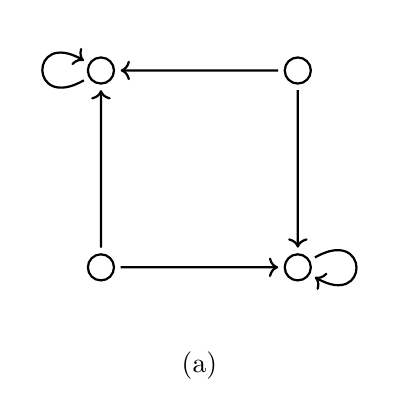
\begin{tikzpicture}[main node/.style={circle,fill=white!20,thick,draw,font=\sffamily\normalsize\bfseries},scale=2.5]
        \node (a) at (1,0) {(a)};
        \node[main node] (1) at (0.5,0.5) {};
        \node[main node] (2) at (0.5,1.5) {};
        \node[main node] (3) at (1.5,0.5) {};
        \node[main node] (4) at (1.5,1.5) {};
        \path[thick]
        (1) edge[->, shorten <= 2pt, shorten >= 2pt] (3)
        (1) edge[->, shorten <= 2pt, shorten >= 2pt] (2)
        (4) edge[->, shorten <= 2pt, shorten >= 2pt] (3)
        (4) edge[->, shorten <= 2pt, shorten >= 2pt] (2)
        (2) edge[->, loop left, distance=10pt, shorten <= 2pt, shorten >= 2pt, thick, in=150, out=210] (2)
        (3) edge[->, loop left, distance=10pt, shorten <= 2pt, shorten >= 2pt, thick, in=-30, out=30] (3);
      \end{tikzpicture}
      &
      \hskip1in

      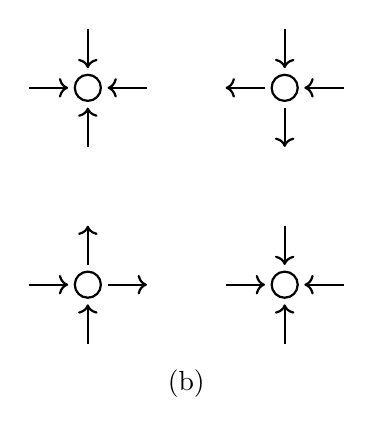
\begin{tikzpicture}[main node/.style={circle,fill=white!20,thick,draw,font=\sffamily\normalsize\bfseries},scale=2.5]
        \node (b) at (1,0) {(b)};
        \node[main node] (1) at (0.5,0.5) {};
        \node[main node] (2) at (0.5,1.5) {};
        \node[main node] (3) at (1.5,0.5) {};
        \node[main node] (4) at (1.5,1.5) {};
        % x1 vector field
        \draw[->, thick] (1.4,1.5)--(1.2,1.5);
        \draw[->, thick] (0.6,0.5)--(0.8,0.5);
        \draw[->, thick] (0.2,0.5)--(0.4,0.5);
        \draw[->, thick] (0.2,1.5)--(0.4,1.5);
        \draw[->, thick] (1.8,0.5)--(1.6,0.5);
        \draw[->, thick] (1.8,1.5)--(1.6,1.5);
        \draw[->, thick] (1.2,0.5)--(1.4,0.5);
        \draw[->, thick] (0.8,1.5)--(0.6,1.5);
        % x2 vector field
        \draw[->, thick] (0.5,0.6)--(0.5,0.8);
        \draw[->, thick] (0.5,1.2)--(0.5,1.4);
        \draw[->, thick] (0.5,1.8)--(0.5,1.6);
        \draw[->, thick] (0.5,0.2)--(0.5,0.4);
        \draw[->, thick] (1.5,0.2)--(1.5,0.4);
        \draw[->, thick] (1.5,1.8)--(1.5,1.6);
        \draw[->, thick] (1.5,0.8)--(1.5,0.6);
        \draw[->, thick] (1.5,1.4)--(1.5,1.2);
      \end{tikzpicture}
      \\
    \end{tabular}
    \caption{(a) State transition graph generated by asynchronous update $\cG \colon \cD \to \cD$ of the monotone Boolean function $f = (f_1, f_2) = ({\bf I}, {\bf I})$ for the network in Figure~\ref{fig:toggle}(a). (b) Labeling of $\cD$ generated by $\cG$. The open circles represent the states of $\cD$ and the arrows represent the labeling.}
    \label{fig:labeling}
  \end{figure}

  %%%%%%%%%%%%%%%%%%%%%%%%%%%%%%%%%%%%%%%%%%%%%%%%%%%%%%%%%%%%%%%%%%%%%%%%%%%%%%%%
  \subsection{Cubical complex}
  \label{section:wall}

  For $n=1,\ldots, N$, let $K(n)$ be a positive integer, set
  \[
    I_n := \setof{0,\ldots, K(n)+1} \subset \Z
  \]
  and define
  \begin{equation}
    \label{eq:II}
    \I := \prod_{n=1}^N I_n\subset \Z^N.
  \end{equation}
  Throughout this manuscript
  \[
    \bv\in \I \quad \text{and} \quad \bq,\bw\in \setof{0,1}^N.
  \]
  Set
  \[
    \dim(\bw) = \sum_{n=1}^N \bw_n.
  \]
  Particular elements of interest in $\setof{0,1}^N$ are
  \[
    {\bf 1}=(1,\ldots, 1), \quad {\bf 0}=(0,\ldots, 0), \quad {\bf 1}^{(n)}=(1,\ldots,1,0,1\ldots 1),
  \]
  where  the $n$-th coordinate is $0$,  and ${\bf 0}^{(n)} = {\bf 1}-{\bf 1}^{(n)}$.

  \begin{defn}
    \label{defn:Xcomplex}
    The $N$-dimensional \emph{cubical cell complex} generated by  $\I$ is denoted by $\cX(\I) = (\cX,\preceq,\dim,\kappa)$ and defined as follows. The set of cells is
    defined by
    \[
      \cX = \setof{ \xi = [\bv,\bw] \mid \bv\in \I, \bw\in \setof{0,1}^N, \text{ and } \bv + \bw \in \I}.
    \]
    The \emph{dimension} of a cell is given by
    \[
      \dim([\bv,\bw]) = \dim(\bw)
    \]
    and we set $\cX^{(n)} := \setof{\xi\in\cX \mid \dim(\xi) = n}$.

    The partial order $\preceq$, called the \emph{face relation}, indicates which cells are faces of other cells and is defined as
    \begin{equation}\label{eq:is_a_face}
      [\bv,\bw]\preceq[\bv',\bw']\ \text{if and only if $\bv = \bv'+\bq$ and $\bw +\bq \bw'$}.
    \end{equation}

    The \emph{incidence number} $\kappa$ is defined by
    \[
      \kappa\left( \left[\bv,\bw \right], \left[ \bv,\bw - {\bf 0}^{(i)}\right] \right) = (-1)^{\sum_{k=1}^i \bw_k}
    \]
    and
    \[
      \kappa\left( \left[\bv,\bw \right], \left[ \bv +{\bf 0}^{(i)} ,\bw - {\bf 0}^{(i)}\right] \right) = - (-1)^{\sum_{k=1}^i \bw_k}
    \]
    under the assumption that $\bw_i = 1$, and $\kappa(\xi, \xi') = 0$ for all other pairs $(\xi, \xi') \in \cX \times \cX$.
  \end{defn}

  \begin{ex}
    \label{ex:cubicalcomplex}
    Consider $N=2$ and assume $K(n)=2$ for $n=1,2$. Then $\I = \prod_{n=1}^2 \setof{0,1,2,3}$. The elements of $\cX$ can be visualized as in Figure~\ref{fig:position_vectors}.
  \end{ex}

  \begin{defn}
    \label{defn:JeJi}
    Let $\cX(\I)$ be a $N$-dimensional cubical cell complex. The \emph{essential} and \emph{inessential} directions of $\xi = [\bv,\bw] \in \cX$ are given by
    \[
      J_e(\xi) = J_e([\bv,\bw]) \coloneqq \setof{n\mid \bw_n=1} \text{ and } J_i(\xi) = J_i([\bv,\bw]) \coloneqq \setof{n\mid \bw_n=0},
    \]
    respectively.
  \end{defn}

  \begin{figure}
    \centering
    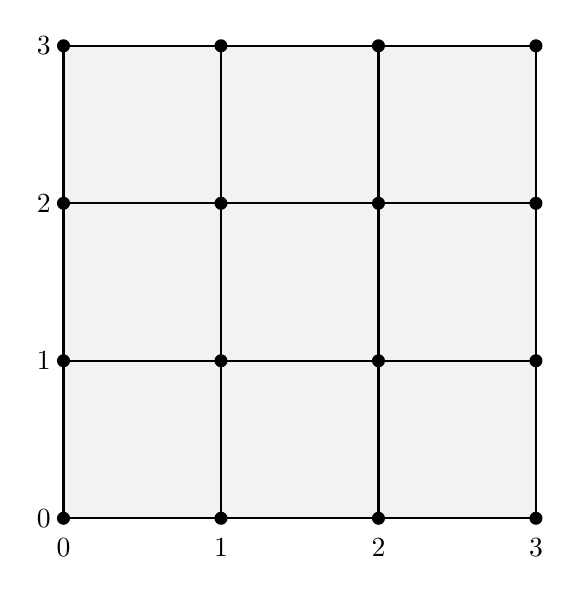
\begin{tikzpicture}[scale=0.25]
      % draw rectangle
      \fill[gray!10!white] (0,0) rectangle (24,24);
      % draw numbers
      \foreach \i in {0,...,3} {
        \draw(8*\i, -1.5) node{$\i$}; % row
        \draw(-1, 8*\i) node{$\i$}; % column
      }
      % Draw the large grid
      \draw[step=8cm,black, thick] (0,0) grid (24,24);
      % zero cells
      \foreach \i in {0,...,3} {
        \foreach \j in {0,...,3} {
          \draw[black, fill=black] (8*\i,8*\j) circle (2ex);
        }
      }
    \end{tikzpicture}
    \caption{A visualization of the abstract cubical cell complex $\cX(\I)$ where $\I = \setof{0,1,2,3}^2$. The vertices and two-dimensional cells of $\cX$ can be expressed as $\defcell{n_1}{n_2}{0}{0}$, for  $n_i\in \setof{0,1,2,3}$, and $\defcell{n_1}{n_2}{1}{1}$, for  $n_i\in \setof{0,1,2}$, respectively. The edges that are visualized as horizontal and vertical segments  take the form $\defcell{n_1}{n_2}{1}{0}$, where $n_1\in \setof{0,1,2}$ and $n_2\in \setof{0,1,2,3}$,  and $\defcell{n_1}{n_2}{0}{1}$, where $n_1\in \setof{0,1,2,3}$ and $n_2\in \setof{0,1,2}$, respectively.}
    \label{fig:position_vectors}
  \end{figure}

  Our characterization of combinatorial dynamics on an $N$-dimensional cubical cell complex $\cX$ is based on information organized using top cells $\cX^{(N)}$.

  \begin{defn}
    \label{defn:wall}
    Given an $N$-dimensional cubical cell complex $\cX$ the set of \emph{top pairs} is given by
    \[
      \TP(\cX) : = \setof{(\xi, \mu) \in \cX \times \cX^{(N)} \mid \xi \preceq \mu}.
    \]
    Of particular interest is the subcollection where $\xi \in \cX^{(N-1)}$.
    The set of \emph{walls} of $\cX$ is
    \[
      W(\cX) := \setof{(\xi, \mu) \in \cX^{(N-1)} \times \cX^{(N)} \mid \xi \prec \mu}.
    \]
    A wall $(\xi, \mu)\in W(\cX)$ is called an \emph{$n$-wall} if $J_i(\xi) = \setof{n}$.
  \end{defn}

  In a slight misuse of language we say that $\xi\in\cX^{(N-1)}$ is a wall of $\mu\in\cX^{(N)}$ to indicate that $(\xi, \mu)$ is a wall.

  A top cell $\mu = [\bv, {\bf 1}] \in \cX^{(N)}$ has two $n$-walls
  for each $n$,
  \[
    \mu^-_n = [\bv, {\bf 1}^{(n)}]\quad \text{and}\quad \mu^+_n = [\bv + {\bf 0}^{(n)}, {\bf 1}^{(n)}],
  \]
  called the \emph{left} and \emph{right $n$-walls} of $\mu$, respectively.
  Two distinct top cells $\mu,\mu'\in\cX^{(N)}$ are \emph{$n$-adjacent} if $\mu$ and $\mu'$ share an \emph{$n$-wall} $\xi$, i.e., $(\xi, \mu)$ and $(\xi, \mu')$ are $n$-walls.

  Let $\xi_0 \in\cX$.
  The \emph{walls} of $\xi_0\in\cX$ are
  \begin{equation*}
    W(\xi_0) := \setof{(\xi, \mu) \in W(\cX) \mid  \xi_0 \preceq \xi}.
  \end{equation*}

  %%%%%%%%%%%%%%%%%%%%%%%%%%%%%%%%%%%%%%%%%%%%%%%%%%%%%%%%%%%%%%%%%%%%%%%%%%%%%%%%
  \subsection{Wall labeling of a cubical complex}
  \label{DSGRN_wall_labeling}

  \begin{defn}
    \label{def:wall_labeling}
    Let $\cX$ be an $N$ dimensional cubical complex.
    A function $\omega \colon W(\cX) \to \setof{\pm 1}$ is a \emph{wall labeling} if for each $\sigma \in \cX^{(0)}$ there exists a map
    \[
      \tilde{o}_{\sigma}\colon \setof{1, \ldots, N} \to \setof{1,\ldots, N},
    \]
    called a \emph{local inducement map}, satisfying the following two conditions.
    \begin{enumerate}
      \item[(i)] Let $\mu, \mu'\in \Top_\cX(\sigma)$ be $n$-adjacent.
        If $k \neq n$ and $k \neq \tilde{o}_\sigma(n)$, then
        \[
          \omega(\mu^-_k, \mu) = \omega(\mu'^-_k, \mu') \quad \text{and} \quad \omega(\mu^+_k, \mu) = \omega(\mu'^+_k, \mu').
        \]
      \item[(ii)] Let $(\xi, \mu)$ and $(\xi, \mu') \in W(\sigma)$ be $n$-walls. If $n \neq \tilde{o}_\sigma(n)$, then
        \[
          \omega(\xi, \mu) = \omega(\xi, \mu').
        \]
    \end{enumerate}
  \end{defn}

  %%%%%%%%%%%%%%%%%%%%%%%%%%%%%%%%%%%%%%%%%%%%%%%%%%%%%%%%%%%%%%%%%%%%%%%%%%%%%%%%
  \subsection{Multi-level labeling induces a wall labeling of cubical complex}
  \label{sec:label_wall_label}

  Given a regulatory network $RN = (V, E, \delta)$ with $V = \{ 1, 2, \ldots, N \}$, we constructed a finite multilevel model $g \colon \cD \to \cD$ where $\cD$ is the set of states
  \[
    \mathcal{D} = \prod_{i = 1}^N \{0, 1, \ldots, m_i\},
  \]
  and $m_i = | \Targets(i) |$ is the number of out-edges of node $i$. For a given parameter $p = (f, \theta) \in \cP$ let $\alpha \colon \cD \times V \times \{ \pm 1\} \to \{\pm 1\}$ be the labeling on $\cD$ given in Definition~\ref{def:multilevel_labeling}.
  Let $K(j) := m_j$ and consider $N$-dimensional cubical complex $\cX$ generated by
  \[
    \I = \prod_{j=1}^N \setof{0, \ldots, K(j) + 1}
  \]
  with set of walls $W(\cX)$. Define $\varphi \colon \cD \to \cX^{(N)}$ by
  \[
    \varphi(v) := [v, {\bf 1}],
  \]
  and notice that $\varphi$ is a bijection. Let
  \begin{equation}
    \label{eq:bijection_Boolean_walls}
    \psi \colon \cD \times V \times \{ \pm 1\} \to W(\cX)
  \end{equation}
  be the map defined by
  \begin{align*}
    & \psi (v, j, -1) := \left( [v, {\bf 1}], [v, {\bf 1}^{(j)}] \right) = (\mu, \mu_j^-) \\
    & \psi (v, j, 1) := \left( [v, {\bf 1}], [v + {\bf 0}^{(j)}, {\bf 1}^{(j)}] \right) = (\mu, \mu_j^+),
  \end{align*}
  where $\mu = \varphi(v) = [v, {\bf 1}] \in \cX^{(N)}$.

  \begin{prop}
    The map $\psi \colon \cD \times V \times \{ \pm 1\} \to W(\cX)$ defined in \eqref{eq:bijection_Boolean_walls} is a bijection.
  \end{prop}

  \begin{proof}
    The map $\psi$ is clearly injective. To show that $\psi$ is surjective, let $(\xi, \mu) \in W(\cX)$ be a wall of $\mu$. It follows that there exists $j \in \{ 1, \ldots, N \}$ such that $J_i(\xi) = \setof{j}$ and hence that $(\xi, \mu)$ is a $j$-wall of $\mu$. Thus $(\xi, \mu)$ is either the left $j$-wall $\mu_j^-$ of $\mu$ or the right $j$-wall $\mu_j^+$ of $\mu$. Let $v = \varphi^{-1}(\mu)$ and notice that in the first case $\psi (v, j, -1) = (\mu, \mu_j^-)$ and in the second case $\psi (v, j, 1) = (\mu, \mu_j^+)$. Therefore $\psi$ is surjective and hence a bijection.
  \end{proof}

  We define a labeling $\omega \colon W(\cX) \to \{ \pm 1\}$ by
  \begin{equation}
    \label{eq:Boolean_wall_labeling}
    \omega (\xi, \mu) := \alpha(\psi^{-1}(\xi, \mu)).
  \end{equation}

  \begin{thm}
    \label{thm:Boolen_wall_label}
    The map $\omega \colon W(\cX) \to \{ \pm 1\}$ defined by \eqref{eq:Boolean_wall_labeling} is a wall labeling.
  \end{thm}

  The following lemma is used in the proof of Theorem~\ref{thm:Boolen_wall_label}. We denote by $e_j$ the unit vector in the $j$-th direction.

  \begin{lem}
    \label{lem:labeling}
    Let $d, d' \in \cD$. If $d - d'= e_j$ for some $j \in \setof{1, \ldots, N}$, then there is an index $k = k(j) \in \setof{1, \ldots, N}$ such that
    \begin{enumerate}[(i)]
      \item For any index $i \neq k$ and $i \neq j$
        \[
          \alpha(d', i, -1) = \alpha(d, i, -1) \quad \text{ and } \quad \alpha(d', i, +1) = \alpha(d, i, +1).
        \]
      \item If $j \neq k$, then
        \[
          \alpha(d', j, +1) = \alpha(d, j, -1).
        \]
    \end{enumerate}
  \end{lem}

  \begin{proof}
    Let $d,d' \in \cD$ be such that $d - d' = e_j$. So $d_j = d'_j + 1$ and $d_i = d'_i$ for $i \neq j$.
    Let $k \in \Targets(j)$ be such that $\theta_j(k) = d_j$. It follows that $d'_j < \theta_j(k)$ and $d_j \geq \theta_j(k)$ and for any $i \neq k$ either $d'_j < \theta_j(i)$ and $d_j < \theta_j(i)$ or $d'_j \geq \theta_j(i)$ and $d_j \geq \theta_j(i)$. Hence for $i \neq k$, by definition, $B^i(d') = B^i(d)$ and thus
    \[
      g_i(d') = \sum_{j \in \Targets(i)} f_i^j(B^i(d')) = \sum_{j \in \Targets(i)} f_i^j(B^i(d)) = g_i(d).
    \]
    Therefore if $i \neq k$ and $i \neq j$ then $g_i(d') = g_i(d)$ and $d_i' = d_i$ and hence $\alpha(d', i, \lambda) = \alpha(d, i, \lambda)$ which proves (i).

    To prove (ii), notice that since $j \neq k$ we have $g_j(d') = g_j(d)$ as above. Hence there are two cases to consider:
    \begin{itemize}
      \item If $g_i(d') = g_i(d) \leq d'_j < d_j$, then $\alpha(d', j, +1) = -1$ and $\alpha(d, j, -1) = -1$.
      \item If $g_i(d') = g_i(d) \geq d_j > d'_j$, then $\alpha(d', j, +1) = 1$ and $\alpha(d, j, -1) = 1$.
    \end{itemize}
    Therefore $\alpha(d', j, +1) = \alpha(d, j, -1)$, which proves (ii).
  \end{proof}

  \begin{proof}[Proof of Theorem~\ref{thm:Boolen_wall_label}]
    To prove the theorem we need to define a local inducement map for $\omega$. To that end, let $\sigma = [\bv, {\bf 0}] \in \cX^{(0)}$, with $\bv = (\bv_1, \ldots, \bv_N)$. Define $\tilde{o}_{\sigma} \colon \setof{1, \ldots, N} \to \setof{1,\ldots, N}$ by
    \[
      \tilde{o}_{\sigma}(j) :=
      \begin{cases}
        \theta^{-1}_j(\bv_j), & \text{if } \bv_j \neq 0 \\
        j,                    & \text{if } \bv_j = 0.
      \end{cases}
    \]
    Notice that $\tilde{o}_{\sigma}(j)$ coincides with the index $k = k(j)$ from Lemma~\ref{lem:labeling}. Notice also that items (i) and (ii) of Lemma~\ref{lem:labeling} match the requirements (i) and (ii) of a wall labeling in Definition~\ref{def:wall_labeling}. Therefore $\tilde{o}_{\sigma}$ defines a local inducement map for $\omega$. This concludes the proof.
  \end{proof}

  %%%%%%%%%%%%%%%%%%%%%%%%%%%%%%%%%%%%%%%%%%%%%%%%%%%%%%%%%%%%%%%%%%%%%%%%%%%%%%%%
  \subsection{Morse graph}
  \label{sec:Morse_graph}

  Let $\cX$ be a finite set and let $\cF \colon \cX \rightrightarrows \cX$ be a multivalued map.

  \begin{defn}
    The directed graph associated with $\cF$ is $G(\cF) = (\cX,E)$ where the set of vertices is $\cX$ and the edges are given by
    \[
      E = \setdef{ (v,v') \in \cX \times \cX }{ v' \in \cF(v) }.
    \]
  \end{defn}

  We define an equivalence relation $\sim$ on $\cX$ by $v \sim v'$ if and only if there exists $v_0, \ldots, v_k \in \cX$ such that $v_0 = v$, $v_k = v'$ and $v_{i} \in \cF(v_{i-1})$ for $i=1,\ldots,k$. The equivalence classes are the \emph{strongly connected components} of $G(\cF)$ and denoted by $\SCC(\cF)$.

  \begin{defn}
    The \emph{condensation graph} of $G(\cF)$ is the graph defined by $\CG(\cF)=(\SCC(\cF),E_{\SCC})$ where
    \[
      E_{\SCC} = \setdef{ (C, C') \in \SCC(\cF) \times \SCC(\cF)}{C \neq C' \text{ and } \exists v \in C, v'\in C' \text{ s.t. } (v,v') \in E }.
    \]
  \end{defn}
  We define a partial order $\preceq$ on $\SCC(\cF)$ by $C \preceq C'$ if and only if $C = C'$ or if there exists $k\geq 0$ and $C_0,\ldots,C_k \in \SCC(\cF)$ such that $C=C_0$, $C'=C_k$ and $(C_i,C_{i-1}) \in E_{\SCC}$ for $i=1,\ldots,k$.

  \begin{defn}
    A strongly connected component $C$ is a \emph{recurrent component} if the subgraph of $G(\cF)$ induced by $C$ contains at least one edge, that is,
    \[
      C \text{ is recurrent} \iff E \cap (C \times C) \neq \emptyset.
    \]
    Let $\RC(\cF)$ denote the set of recurrent components of $G(\cF)$.
  \end{defn}

  \begin{defn}
    The Morse Graph of $\cF$, $\MG(\cF)$, is the partially ordered set $(\RC(\cF), \preceq)$.
  \end{defn}

  We represent the Morse graph as the transitive reduction of the directed acyclic graph defined by the poset $(\RC(\cF), \preceq)$, that is, we define a directed acyclic graph whose vertices are $\RC(\cF)$ and edges are $\setdef{(C, C') \in \RC(\cF) \times \RC(\cF)}{C' \prec C}$ and represent $\MG(\cF)$ as the transitive reduction of this graph. This representation of the Morse graph is called the Hasse diagram of the poset $(\RC(\cF),\preceq)$.

  \begin{defn}
    \label{def:Boolean_MG}
    The \emph{Boolean Morse graph} of a monotone Boolean model $f \colon \bbB^N \to \bbB^N$ is the Morse graph $\MG(\cF)$ of the multivalued map $\cF \colon \bbB^N \rightrightarrows \bbB^N$ given by Definition~\ref{def:Boolean_update}. We call a node in the Morse graph $\MG(\cF)$ a \emph{Fixed Point}, and label it as $FP(b)$, if the corresponding strongly connected component consists of a single state $b \in \bbB^N$. Otherwise we call it a \emph{Full Cycle} and label it as $FC$.
  \end{defn}

  \begin{defn}
    \label{def:multi_Boolean_MG}
    The \emph{Multilevel Boolean Morse graph} of a regulatory network $RN$ at a parameter $(f, \theta) \in \PG$ is the Morse graph $\MG(\cG)$ of the multivalued map $\cG \colon \cD \rightrightarrows \cD$ given by Definition~\ref{def:update}. We call a node in the Morse graph $\MG(\cG)$ a \emph{Fixed Point}, and label it as $FP(d)$, if the corresponding strongly connected component consists of a single state $d \in \cD$. Otherwise we call it a \emph{Full Cycle} and label it as $FC$.
  \end{defn}

  A DSGRN parameter $(f, \theta) \in \PG$ gives rise, via equation \eqref{eq:Boolean_wall_labeling}, to a wall labeling $\omega \colon W(\cX) \to \{ \pm 1\}$ which in turn generates a multivalued map $\cF \colon \cX \rightrightarrows \cX$ on the the cubical complex $\cX$ defined in Definition~\ref{defn:Xcomplex} (see \cite{rook_field:24} for details). The multivalued map $\cF \colon \cX \rightrightarrows \cX$ generate the \emph{DSGRN Morse graph} as defined below.

  \begin{rem}
    \label{DSGRN_STG}
    A wall labeling $\omega \colon W(\cX) \to \{ \pm 1\}$ actually generates five multivalued maps $\cF_i \colon \cX \rightrightarrows \cX$, $i = 0, 1, \ldots, 4$, at different levels of refinement (see \cite{rook_field:24}). For the computations in this paper we use the most refined multivalued map $\cF_4 \colon \cX \rightrightarrows \cX$ (see Section~\ref{sec:code}). In this paper we refer to this map simply as $\cF \colon \cX \rightrightarrows \cX$.
  \end{rem}

  The methods presented in \cite{rook_field:24} also includes the computation of the \emph{Conley index} of each strongly connected component. The Conley index can be used to characterize the dynamics corresponding to the Morse graph nodes and is used to label the nodes of the Morse graph as defined below.

  \begin{defn}
    \label{def:DSGRN_MG}
    The \emph{DSGRN Morse graph} of a regulatory network $RN$ at a parameter $(f, \theta) \in \PG$ is the Morse graph $\MG(\cF)$ of the DSGRN multivalued map $\cF \colon \cX \rightrightarrows \cX$ defined above. Let $q$ be a node in the Morse graph $\MG(\cF)$ and let $k$ denote the number of cells in the corresponding strongly connected component. We assign to node $q$ the label $\ell(q)$ defined by
    \[
      \ell(q) :=
      \begin{cases}
        FP(k), & \text{if}~ q ~\text{has the Conley index of a fixed point} \\
        PO(k), & \text{if}~ q ~\text{has the Conley index of a periodic orbit} \\
        T(k),  & \text{if}~ q ~\text{has the trivial Conley index} \\
        M(k),  & {otherwise}.
      \end{cases}
    \]
  \end{defn}

  \begin{rem}
    For the multivalued map $\cF \colon \cX \rightrightarrows \cX$, defined in \cite{rook_field:24}, there is a notion of a gradient direction which can be used to conclude that some recurrent components are trivial (in the sense that they do not represent any dynamics of the model). So we define $\GRC(\cF)$ as the set of recurrent components in $\RC(\cF)$ for which there is common gradient direction and define the Morse graph as $\MG(\cF) := \RC(\cF) \setminus \GRC(\cF)$ with partial order $\preceq$.
  \end{rem}

  %%%%%%%%%%%%%%%%%%%%%%%%%%%%%%%%%%%%%%%%%%%%%%%%%%%%%%%%%%%%%%%%%%%%%%%%%%%%%%%%
  \subsection{Multilevel refinement of Boolean models}

  Let $RN$ be a regulatory network with $V = \setof{1, \ldots, N}$ and $f \colon \bbB^N \to \bbB^N$ be a monotone Boolean model. Recall that a DSGRN parameter is defined in terms of monotone increasing Boolean functions (see Definition~\ref{def:fi}). Recall also that associated to $f$ there is an increasing monotone Boolean model $\tilde{f}$ via by the change of variables $\beta$ in \eqref{eq:beta}. Hence there are two multivalued maps associated to $f$.

  One is the asynchronous update multivalued map $\cF \colon \bbB^N \rightrightarrows \bbB^N$ generated by $f$, given by Definition~\ref{def:Boolean_update}, which gives rise to the Boolean dynamics of the network.

  The other is the nearest neighbor asynchronous update multivalued map $\cG \colon \cD \rightrightarrows \cD$ (see Definition~\ref{def:update}), which is used to compute the finite multilevel dynamics of the network. The map $\cG$ is defined in terms of a DSGRN parameter as follows. Given an order parameter $\theta$, the map $\tilde{f}$ defines a Boolean DSGRN parameter $(\hat{f}, \theta) \in \PG$, where
  \[
    \hat{f} = \left( (\tilde{f}_1, \ldots, \tilde{f}_1), (\tilde{f}_2, \ldots, \tilde{f}_2), \ldots, (\tilde{f}_N, \ldots, \tilde{f}_N) \right),
  \]
  as defined by \eqref{eq:Boolean_par}. The parameter $(\hat{f}, \theta)$ is then used to define the finite multilevel update function $g \colon \cD \to \cD$ given by \eqref{Psi}, which in turn generates the nearest neighbor asynchronous update multivalued map $\cG \colon \cD \rightrightarrows \cD$.

  The goal of this section is to show that for the Boolean parameter $p = (\hat{f}, \theta)$ the labeling $\alpha$ generated by the finite multilevel update function $g$ is a multilevel refinement of the Boolean map $f$.

  Given two configurations $d, d' \in \cD$, the components that differ are denoted by $\Delta(d, d') := \setdef{i \in \{1, \ldots, N\} }{d_i\not = d'_i}$.

  We now define a notion of a multivalued refinement of a Boolean model $f \colon \bbB^N \to \bbB^N$. The refinement criteria relies on a binarization of the multivalued configurations $d \in \cD$. A binarization $\mu \colon \cD \to \bbB^N$ has the form
  \[
    \mu(d) = (\mu_1(d_1), \mu_2(d_2), \ldots, \mu_n(d_n)),
  \]
  where $\mu_i \colon X_i \to \bbB$ with $X_i := \{0, 1, \ldots, m_i\}$. We require that a binarization satisfies
  \[
    \mu_i(0) = 0 \quad \mbox{ and } \quad \mu_i(m_i)=1, \quad \forall i \in \{ 1, 2, \ldots, N\},
  \]
  and that $\mu_i$ is monotone increasing. Let  $M(d)$ be the set of all possible binarizations of a configuration $d \in \cD$, that is,
  \Bernardo{$M(k)$ is Morse node label}
  \[
    M(d) := \setdef{b \in \bbB^N}{b = \mu(d) ~\text{for some binarization}~ \mu \colon \cD \to \bbB^N}.
  \]

  \begin{defn}[{\bf Multivalued refinement}\cite{Pauleve_MP}]
    A  multilevel function $g \colon \cD \to \cD$ is a \emph{multilevel refinement} of a Boolean model $f \colon \bbB^N \to \bbB^N$, $f = (f_1, \ldots, f_n)$, if and only if the labeling $\alpha$ on $\Omega$ generated by $g$ satisfies the following properties for every $(d, j, \pm 1) \in \Omega$ and every $i \in \{ 1, 2, \ldots, N \}$:
    \begin{enumerate}[(i)]
      \item If $\alpha(d,j, \pm 1) = 1$, then there exists $b \in M(d)$ such that $f_i(b) = 1$;
      \item If $\alpha(d,j, \pm 1) = -1$, then there exists $b \in M(d)$ such that $f_i(b) =0$.
    \end{enumerate}
  \end{defn}

  \begin{thm}
    Let $RN$ be a regulatory network with $V = \{ 1, \ldots, N \}$. Let $f \colon \bbB^N \to \bbB^N$ be a Boolean model and let $(\hat{f}, \theta) \in \PG$ be a corresponding parameter node as defined above. Let $g \colon \cD \to \cD$ be the multilevel function defined by $(\hat{f}, \theta)$. Then $g$ is a multilevel refinement of the Boolean model $f$.
  \end{thm}

  \corrc MG: To here. I still need to adjust the notation of the proof to the notation above.
  <<>>

  \begin{proof}
    Let $x \in D$ and fix $i \in [n]$.% with $1 < x_i < m_i$. \Tomas{ discuss $x_i=0, m_i$}

    \begin{description}
      \item[(a)]  Assume first that
        \[ \alpha(d, i, 1) = 1.\]
        This choice implies that  $d_i < m_i$ and by Definition~\ref{def:multilevel_labeling} this implies
        $g_i(d) >d_i.$
        From the commutative diagram (\ref{comm:diag}) this implies that
        \begin{align*}
          \sum_{j \in \Targets(v_i)} f_i^j(B(d))& >d_i \\
          |\Targets(v_i)|f_i(B(d))& >d_i \\
          m_i f_i(B(d))& >d_i
        \end{align*}
        where the second line follows from the choice of Boolean parameter where $f_i^j = f_i$ for all $j = 1, \ldots, m_i$.
        Since the value of Boolean function $f_i \in \{0,1\}$ this implies
        \begin{equation}\label{one}
          f_i(B(d)) = 1.
        \end{equation}

      \item[(b)] Assume now that
        \[ \alpha(d, i, -1) = 1.\]
        This choice implies that  $d_i >0 $.

        From Definition~\ref{def:multilevel_labeling} this implies
        either that the first line is applicable and thus
        \[ g_i(d) >d_i,\]
        or the third line is valid and
        \[ g_i(d) =d_i.\]
        In the first case, the argument in (a) applies and  (\ref{one}) holds.
        In the second case, the commutative diagram (\ref{comm:diag}) implies that
        \[
          \sum_{j \in \Targets(v_i)} f_i^j(B(d)) =x_i \quad \mbox{ which implies } \quad
        m_i f_i(B(d)) =d_i .\]
        Since $d_i>0$  this again implies  (\ref{one}).

      \item[(c)] Assume  that
        \[ \alpha(d, i, -1) = -1.\]
        This choice implies that  $d_i >0$.
        From Definition~\ref{def:multilevel_labeling} this implies
        $g_i(d) <d_i.$
        From the commutative diagram this implies that
        \begin{align*}
          \sum_{j \in \Targets(v_i)} f_i^j(B(d))& <d_i \\
          |\Targets(v_i)|f_i(B(d))& <d_i \\
          m_i f_i(B(d))& <d_i
        \end{align*}
        where the second line follows from the choice of Boolean parameter where $f_i^j = f_i$ for all $j = 1, \ldots, m_i$.
        Since the value of Boolean function $f_i \in \{0,1\}$ this implies
        \begin{equation}\label{two}
          f_i(B(d)) = 0.
        \end{equation}

      \item[(d)] Finally, we assume
        \[ \alpha(d, i, 1) = -1.\]
        This choice implies that  $d_i <m_i $.
        From Definition~\ref{def:multilevel_labeling}
        there are two possibilities.
        First, for state $y$ which differs from $x$ in $i-$th direction that is $y_i= x_i+1$ and $ y_j=x_j, j\not = i$, we have $g_i(y) <y_i$.
        Then the argument in part $c$ reads
        \begin{align*}
          \sum_{j \in \Targets(v_i)} f_i^j(B(y))& <y_i \\
          |\Targets(v_i)|f_i(B(y))& <y_i \\
          m_i f_i(B(y))& <y_i
        \end{align*}
        and  (\ref{two}) holds for state $y$. Note that $y_i \leq m_i$.

        Second possibility in Definition~\ref{def:multilevel_labeling}  is that
        \[ g_i(d) =d_i.\]
        From the commutative diagram (\ref{comm:diag}) this implies
        \[
          \sum_{j \in \Targets(v_i)} f_i^j(B(d)) =d_i \quad \mbox{ which implies } \quad
        m_i f_i(B(d)) =d_i .\]
        This implies (\ref{two}).
    \end{description}

    To finish the proof, we define for every $d$ a state $d' \in \bbB^n$ such that
    \[ f_i(B(d)) = f_i(d') \quad \mbox{ for all } i \in [n].\]

  We first note that in the expression  $f_i(B(d))$ the  value of $B(d) \in \bbB^{|E|}$ assigns a Boolean value to each network edge $e \in E$. For any edge $e$ we denote by $[B(d)]_e$ the $e$th component of the vector $B(d)$. Since for Boolean parameter $f_i^j=f_i$ for all $j \in \Targets)(v_i)$ we set
  \begin{equation} \label{eq:xprime}
    d_i' = f_i(B(d)).
  \end{equation}
  Consider now an abitrary function $f_j(B(d))$. Then the value of $f_j(B(d))$ depends on the values of the input edges
  \[ f_j(B(d)) =f_j(\{ [B(d)]_{v_k \multimap v_j}\}_{k\in \Sources(v_j)}) \]
  which in turn are values of the functions $f_k^j$ for $k \in \Sources(v_j)$
  \[ =f_j(\{ [B(d)]_{v_k \multimap v_j}\}_{k\in \Sources(v_j)})= f_j(\{ f_k^j(B(d))\}_{k\in \Sources(v_j)}) .\]
  Since for all $j$ we have $f_k^j=f_k$ for Boolean parameter, it follows that
  \[ f_j(\{ f_k^j(B(d))\}_{k\in \Sources(v_j)}) = f_j(\{f_k(B(d))\}_{k\in \Sources(v_j)}).\]
  By (\ref{eq:xprime})
  \[  f_j(\{f_k(B(d))\}_{k\in \Sources(v_j)})= f_j(\{d'_k\}_{k\in \Sources(v_j)}). \]
  Since $j$ was arbitrary,
  \[ f(B(d)) = f(d'), \quad \mbox{ for } x'\in \bbB^n \quad \mbox{ defined in} (\ref{eq:xprime}).\]
  This shows that for Boolean parameter $(f,\theta) \in \PG$, the induced multivalued function $g$ is multivalued refinement of the Boolean function $f$.
\end{proof}

%%%%%%%%%%%%%%%%%%%%%%%%%%%%%%%%%%%%%%%%%%%%%%%%%%%%%%%%%%%%%%%%%%%%%%%%%%%%%%%%
\subsection{Additional examples}
\label{sec:more_examples}
{\color{magenta}

  Do a big calculation like p53.
  I would select Boolean model where whenever there is a negative input it is dominant and positive inputs add.
  This is the default that biologists often use when they do these models and what we have used and that led to sums of products.
  so
  \begin{itemize}
    \item at MDM the function is identity( MDM: p53)
    \item at Wip1 also identity ( wip1: p53)
    \item at chk2 the function is (chk2: ATM AND not wip1)
    \item at ATM  it is minus identity  (ATM: Not Wip1)
    \item at p53  (p53: ((ATM or Chk) and not MDM2)
    \end{itemize}

    Run this particular Boolean model  on Gin sim
    identify the dynamics of the same parameter in DSGRN

    Then compare this to statistics of dynamics
    \begin{itemize}
      \item at all
        MBF parameters
      \item essential MBF parameters
      \item dynamics in  1-neighborhood of the Boolean model.
      \item dynamics with the same Boolean logic but different orders of parameters (this should be only 4 parameters since only ATM and p53 have two out-edges.
      \end{itemize}
    }

    %%%%%%%%%%%%%%%%%%%%%%%%%%%%%%%%%%%%%%%%%%%%%%%%%%%%%%%%%%%%%%%%%%%%%%%%%%%%%%%%
    \section{Conclusions}

    %%%%%%%%%%%%%%%%%%%%%%%%%%%%%%%%%%%%%%%%%%%%%%%%%%%%%%%%%%%%%%%%%%%%%%%%%%%%%%%%
    \section{Lattices of monotone increasing Boolean functions}

    \corrc MG: I think we don't need this material in Section~\ref{sec:math} so I moved it here (I will move it back there if needed). I think this should be an appendix and we should also have another appendix with a discussion of the different incarnations of the DSGRN parameter graph.
    <<>>

    \corrc TG: I do not think the lattice structure is needed in this paper. It has been described elsewhere.
    Since this paper is meant as an introduction/review paper, maybe I will add this as just a remark with a reference.
    <<>>

    \begin{defn}
      The set of monotone increasing Boolean functions with $k$ inputs $f \colon \bbB^k \to \bbB$ is denoted by $\cM_k$.
    \end{defn}

    \begin{defn}
      The \emph{truth set} of a monotone Boolean function $f \colon \bbB^k \to \bbB$ is defined as
      \[
        \cT(f) :=\{ z \in \bbB^k \;|\; f(z) =1 \}.
      \]
    \end{defn}

    The set $\cM_k$ forms a lattice, where the join ($\vee$) and meet ($\wedge$) operations are defined by union and intersection of the corresponding truth sets, i.e.,
    \begin{align*}
      h = f \vee g   & \iff \cT(h) = \cT(f) \cup \cT(g), \\
      h = f \wedge g & \iff \cT(h) = \cT(f) \cap \cT(g).
    \end{align*}

    The lattices $\cM_1, \cM_2$ and $\cM_3$ are shown in Figure~\ref{fig:mbf}.

    \begin{figure}[htp!]
      \centering
      \begin{tabular}{cc}
        \begin{tikzpicture}[scale=0.33\textwidth, node distance = .3cm]
          \tikzset{my node/.style = {circle, draw, very thick, inner sep=1pt,minimum size=0pt}}
          \node[my node] (7) {
            \begin{tikzpicture}[node distance = .2cm]
              \tikzset{my node/.style = {circle, draw, inner sep=1pt,minimum size=0pt}}
              \node (A) {$\mathbf{1}$};
            \end{tikzpicture}
          };
          \node[my node,blue] (8) [below=of 7] {
            \begin{tikzpicture}[ node distance = .2cm]
              \tikzset{my node/.style = {circle,draw, inner sep=1pt,minimum size=0pt}}
              \node[black] (2){ \small  $X$};
            \end{tikzpicture}
          };
          \node[my node] (9) [below= of 8] {
            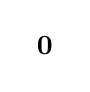
\begin{tikzpicture}[ node distance = .2cm]
              \tikzset{my node/.style = {circle, draw, inner sep=1pt,minimum size=0pt}}
              \node (3){$\mathbf{0}$};
            \end{tikzpicture}
          };
          \node(a)[below=of 9] { (a) };

          \node[my node] (1)[below=of a]  {
            \begin{tikzpicture}[node distance = 0.2cm]
              \tikzset{my node/.style = {circle, draw, inner sep=1pt,minimum size=0pt}}
              \node (A) {$1$};
            \end{tikzpicture}
          };
          \node[my node,blue] (2) [below=of 1] {
            \begin{tikzpicture}[ node distance = .2cm]
              \tikzset{my node/.style = {circle,draw, inner sep=1pt,minimum size=0pt}}
              \node[black] (2){ \tiny  $ X\vee Y$};
            \end{tikzpicture}
          };
          \node[my node] (3) [below left=0.9 and 0.5 of 2] {
            \begin{tikzpicture}[ node distance = .2cm]
              \tikzset{my node/.style = {circle, draw, inner sep=1pt,minimum size=0pt}}
              \node[black]  (3){  $X$};
            \end{tikzpicture}
          };
          \node[my node] (4) [below right=0.9 and 0.5 of 2] {
            \begin{tikzpicture}[ node distance = .2cm]
              \tikzset{my node/.style = {circle, draw, inner sep=1pt,minimum size=0pt}}
              \node (4){  $Y$};
            \end{tikzpicture}
          };
          \node[my node,blue] (5) [below left=0.9 and 0.5 of 4] {
            \begin{tikzpicture}[ node distance = .2cm]
              \tikzset{my node/.style = {circle, draw, inner sep=1pt,minimum size=0pt}}
              \node[black] (5){ \tiny $X \wedge Y$};
            \end{tikzpicture}
          };
          \node[my node] (6) [below=of 5] {
            \begin{tikzpicture}[node distance = .2cm]
              \tikzset{my node/.style = {circle, draw, inner sep=1pt,minimum size=0pt}}
              \node  (6){  $0$};
            \end{tikzpicture}
          };
          \tikzset{my edge/.style = {-, very thick}}
          \draw[my edge] [] (1) to [] (2);
          \draw[my edge] [] (2) to [] (4);
          \draw[my edge] [] (2) to [] (3);
          \draw[my edge] [] (4) to [] (5);
          \draw[my edge] [] (3) to [] (5);
          \draw[my edge] [] (5) to [] (6);
          \draw[my edge] [] (7) to [] (8);
          \draw[my edge] [] (8) to [] (9);
        \end{tikzpicture}
        &
        \begin{tikzpicture}[scale=0.33\textwidth,node distance = .3cm]
          \tikzset{my node/.style = {circle, draw, very thick, inner sep=0pt,minimum size=0pt}}

          \node[my node] (1) {
            \begin{tikzpicture}[node distance = .2cm]
              \tikzset{my node/.style = {circle, draw, inner sep=1pt,minimum size=0pt}}
              \node (A) {\tiny $\mathbf{1}$};
            \end{tikzpicture}
          };
          \node[my node,blue] (2) [below=of 1] {
            \begin{tikzpicture}[ node distance = .2cm]
              \tikzset{my node/.style = {circle,draw, inner sep=1pt,minimum size=0pt}}
              \node[black] (2){ \tiny $X\vee Y\vee Z$};
            \end{tikzpicture}
          };
          \node[my node] (3) [below=of 2] {
            \begin{tikzpicture}[ node distance = .2cm]
              \tikzset{my node/.style = {circle, draw, inner sep=1pt,minimum size=0pt}}
              \node (3){\tiny $X \vee Y$};
            \end{tikzpicture}
          };
          \node[my node] (4) [left=of 3] {
            \begin{tikzpicture}[ node distance = .2cm]
              \tikzset{my node/.style = {circle, draw, inner sep=1pt,minimum size=0pt}}
              \node (4){ \tiny $X \vee Z$};
            \end{tikzpicture}
          };
          \node[my node] (5) [right=of 3] {
            \begin{tikzpicture}[ node distance = .2cm]
              \tikzset{my node/.style = {circle, draw, inner sep=1pt,minimum size=0pt}}
              \node (5){ \tiny $Y \vee Z$};
            \end{tikzpicture}
          };
          \node[my node,blue] (6) [below=of 3] {
            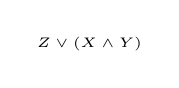
\begin{tikzpicture}[node distance = .2cm]
              \tikzset{my node/.style = {circle, draw, inner sep=1pt,minimum size=0pt}}
              \node[black]  (6){ \tiny $Z \vee (X \wedge Y)$};
            \end{tikzpicture}
          };
          \node[my node,blue] (7) [left=of 6] {
            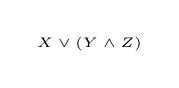
\begin{tikzpicture}[node distance = .2cm]
              \tikzset{my node/.style = {circle, draw, inner sep=1pt,minimum size=0pt}}
              \node[black]  (7){\tiny $X \vee (Y \wedge Z)$};
            \end{tikzpicture}
          };
          \node[my node,blue] (8) [right=of 6] {
            \begin{tikzpicture}[node distance = .2cm]
              \tikzset{my node/.style = {circle, draw, inner sep=1pt,minimum size=0pt}}
              \node[black]  (8){\tiny  $Y \vee (X \wedge Z)$};
            \end{tikzpicture}
          };
          \node[my node] (9) [below left=0.7 and 0.5 of 6] {
            \begin{tikzpicture}[node distance = .2cm]
              \tikzset{my node/.style = {circle, draw, inner sep=1pt,minimum size=0pt}}
              \node (9){ \tiny $Z$};
            \end{tikzpicture}
          };
          \node[my node,blue] (10) [below=of 6] {
            \begin{tikzpicture}[node distance = .2cm]
              \tikzset{my node/.style = {circle, draw, inner sep=1pt,minimum size=0pt}}
              \node[black]  (10){ \tiny $\alpha$};
            \end{tikzpicture}
          };
          \node[my node] (11) [below right=0.9 and 0.1 of 8] {
            \begin{tikzpicture}[node distance = .2cm]
              \tikzset{my node/.style = {circle, draw, inner sep=1pt,minimum size=0pt}}
              \node (11){ \tiny $Y$};
            \end{tikzpicture}
          };
          \node[my node] (12) [below left=0.9 and 0.5 of 7] {
            \begin{tikzpicture}[node distance = .2cm]
              \tikzset{my node/.style = {circle, draw, inner sep=1pt,minimum size=0pt}}
              \node (12){\tiny  $X$};
            \end{tikzpicture}
          };
          \node[my node,blue] (13) [below right=0.9cm and .5cm of 9] {
            \begin{tikzpicture}[node distance = .2cm]
              \tikzset{my node/.style = {circle, draw, inner sep=1pt,minimum size=0pt}}
              \node[black]  (13){ \tiny $(X\wedge Z) \vee (Y \wedge Z)$};
            \end{tikzpicture}
          };
          \node[my node,blue] (14) [right=of 13] {
            \begin{tikzpicture}[node distance = .2cm]
              \tikzset{my node/.style = {circle, draw, inner sep=1pt,minimum size=0pt}}
              \node (14){ \tiny $(X\wedge Y) \vee (Y \wedge Z)$};
            \end{tikzpicture}
          };
          \node[my node,blue] (15) [left=of 13] {
            \begin{tikzpicture}[node distance = .2cm]
              \tikzset{my node/.style = {circle, draw, inner sep=1pt,minimum size=0pt}}
              \node[black]  (15){ \tiny  $(X\wedge Y) \vee (X \wedge Z)$};
            \end{tikzpicture}
          };
          \node[my node] (16) [below=of 13] {
            \begin{tikzpicture}[node distance = .2cm]
              \tikzset{my node/.style = {circle, draw, inner sep=1pt,minimum size=0pt}}
              \node (16){ \tiny$ X \wedge Y$};
            \end{tikzpicture}
          };
          \node[my node] (17) [right=of 16] {
            \begin{tikzpicture}[node distance = .2cm]
              \tikzset{my node/.style = {circle, draw, inner sep=1pt,minimum size=0pt}}
              \node (17){ \tiny $Y\wedge Z$};
            \end{tikzpicture}
          };
          \node[my node] (18) [left=of 16] {
            \begin{tikzpicture}[node distance = .2cm]
              \tikzset{my node/.style = {circle, draw, inner sep=1pt,minimum size=0pt}}
              \node (18){ \tiny  $X \wedge Z$};
            \end{tikzpicture}
          };
          \node[my node,blue] (19) [below=of 16] {
            \begin{tikzpicture}[node distance = .2cm]
              \tikzset{my node/.style = {circle, draw, inner sep=1pt,minimum size=0pt}}
              \node[black]  (19){ \tiny $X\wedge Y\wedge Z$};
            \end{tikzpicture}
          };
          \node[my node] (20) [below=of 19] {
            \begin{tikzpicture}[node distance = .2cm]
              \tikzset{my node/.style = {circle, draw, inner sep=1pt,minimum size=0pt}}
              \node (20){\tiny $\mathbf{0}$};
            \end{tikzpicture}
          };

          \tikzset{my edge/.style = {-, very thick}}
          \draw[my edge] [] (1) to [] (2);
          \draw[my edge] [] (2) to [] (4);
          \draw[my edge] [] (2) to [] (3);
          \draw[my edge] [] (2) to [] (5);
          \draw[my edge] [] (4) to [] (7);
          \draw[my edge] [] (4) to [] (6);
          \draw[my edge] [] (3) to [] (7);
          \draw[my edge] [] (3) to [] (8);
          \draw[my edge] [] (5) to [] (6);
          \draw[my edge] [] (5) to [] (8);
          \draw[my edge] [] (7) to [] (12);
          \draw[my edge] [] (7) to [] (10);
          \draw[my edge] [] (6) to [] (9);
          \draw[my edge] [] (6) to [] (10);
          \draw[my edge] [] (8) to [] (10);
          \draw[my edge] [] (8) to [] (11);
          \draw[my edge] [] (12) to [] (15);
          \draw[my edge] [] (9) to [] (13);
          \draw[my edge] [] (11) to [] (14);
          \draw[my edge] [] (10) to [] (15);
          \draw[my edge] [] (10) to [] (13);
          \draw[my edge] [] (10) to [] (14);
          \draw[my edge] [] (15) to [] (18);
          \draw[my edge] [] (15) to [] (16);
          \draw[my edge] [] (13) to [] (18);
          \draw[my edge] [] (13) to [] (17);
          \draw[my edge] [] (14) to [] (16);
          \draw[my edge] [] (14) to [] (17);
          \draw[my edge] [] (18) to [] (19);
          \draw[my edge] [] (16) to [] (19);
          \draw[my edge] [] (17) to [] (19);
          \draw[my edge] [] (19) to [] (20);
        \end{tikzpicture}
        \\
        (b) &
        (c)
      \end{tabular}
      \caption{ Lattices of Monotone Boolean functions  with (a) $1$ input; (b) $2$ inputs; and  (c) $3$ inputs. Blue circles indicate non-degenerate MBFs.}
      \label{fig:mbf}
    \end{figure}

    %%%%%%%%%%%%%%%%%%%%%%%%%%%%%%%%%%%%%%%%%%%%%%%%%%%%%%%%%%%%%%%%%%%%%%%%%%%%%%%%
    \section{Code Usage}
    \label{sec:code}

    There are two versions of DSGRN. The original version (\texttt{DSGRN}) did not include the blow-up dynamics that can introduce additional fixed points at threshold locations, such as the examples in Fig~\ref{fig:order_flow}. It instead provides multi-level model dynamics as in Figs~\ref{fig:multi1}(c) and~\ref{fig:multi2}(c). These dynamics encompass all Boolean dynamics, and include the identification of multi-cell attractors and unstable strongly connected multi-cell sets in the discrete system.
    The blow-up version (\texttt{DSGRN\_utils}, also called DSGRN-Con) provides the coarse characterization of (more) stable and unstable Morse sets that arise from the assumption of continuity in the underlying dynamical system. The information available is far richer than that in the original DSGRN.

    In this section, we provide a practical guide to using the DSGRN software for analyzing regulatory networks. All mathematical definitions and notation are established in Section~\ref{sec:math}. We demonstrate the workflow through the toggle switch network from Section~\ref{subsec:TS}.

    %%%%%%%%%%%%%%%%%%%%%%%%%%%%%%%%%%%%%%%%%%%%%%%%%%%%%%%%%%%%%%%%%%%%%%%%%%%%%%%%

    \subsection{Defining the Network}

    The first step is defining a regulatory network $\bRN = (V, E, \delta)$ (Definition~\ref{def:RN}) using a string-based format. Each line specifies a node and its regulators:

    \begin{lstlisting}
    import DSGRN

    # Toggle switch network from Section 2.2
    network_spec = """
    x : ~y
    y : ~x
    """
    network = DSGRN.Network(network_spec)
    \end{lstlisting}

    The algebraic expression specifies network topology and edge signs only---not the Boolean logic function. Syntax:
    \begin{itemize}
    \item Activating regulation: \texttt{x} or \texttt{x +}
    \item Repressing regulation: \texttt{\textasciitilde x}
    \item Multiple inputs: \texttt{x + \textasciitilde z}
    \end{itemize}

    Optional modifiers restrict parameter space:
    \begin{itemize}
    \item \texttt{: E} restricts to essential MBFs (all inputs required)
    \item \texttt{: MBF} restricts to monotone Boolean functions only
    \end{itemize}

    %%%%%%%%%%%%%%%%%%%%%%%%%%%%%%%%%%%%%%%%%%%%%%%%%%%%%%%%%%%%%%%%%%%%%%%%%%%%%%%%

    \subsection{Exploring the Parameter Graph}

    The parameter graph $\PG = (\cP, \cE)$ (Section~\ref{sec:PG}) organizes all DSGRN parameters $p = (f, \theta) \in \cP$, where each parameter specifies logic functions $f_i$ (Definition~\ref{def:fi}) and threshold orderings $\theta_i$ for all nodes:

    \begin{lstlisting}
    # Create parameter graph
    parameter_graph = DSGRN.ParameterGraph(network)
    print(f"Total parameters: {parameter_graph.size()}")

    # Access a specific parameter
    parameter_index = 0
    parameter = parameter_graph.parameter(parameter_index)
    print(parameter)  # Shows parameter inequalities
    \end{lstlisting}

    Each parameter $p$ defines a multilevel update function $g \colon \cD \to \cD$ (equation~\eqref{Psi}) operating on the state space $\cD = \prod_{i=1}^{N} X_i$ where $X_i = \{0, 1, \ldots, m_i\}$ and $m_i = |\Targets(i)|$.

    \subsubsection{Interpreting Parameter Inequalities}

    The parameter inequalities specify when each edge is ``turned on'' (Definition~\ref{def:turn_on}). For an activating edge $v_i \to v_j$ with single threshold:
    \[
    L_0 < \theta_1 < L_1
    \]
    the node $v_j$ is OFF when $L < \theta_1$ (input below threshold) and ON when $L > \theta_1$ (input above threshold). For a repressing edge $v_i \dashv v_j$, the threshold ordering reverses: $L_1 < \theta_1 < L_0$.

    For multiple inputs, subscripts on logic parameters $L_{b_1 \cdots b_k}$ indicate input states. The ordering of $L$ values relative to thresholds determines the Boolean function. For example, if node $y$ has algebraic expression \texttt{y : x + \textasciitilde z}, then parameter inequalities $L_{00} < L_{01} < \theta_1 < L_{10} < L_{11}$ correspond to the Boolean function $y = x \wedge \neg z$.

    %%%%%%%%%%%%%%%%%%%%%%%%%%%%%%%%%%%%%%%%%%%%%%%%%%%%%%%%%%%%%%%%%%%%%%%%%%%%%%%%

    \subsection{Computing Dynamics}

    For a given parameter $p \in \cP$, the dynamics are computed using the \texttt{DSGRN\_utils} package, which implements the blow-up dynamics described in~\cite{rook_field:24}.

    \subsubsection{Morse Graphs}

    The Morse graph $\MG(\cF)$ (Definition~\ref{def:DSGRN_MG}) compresses the state transition graph into its recurrent components:

    \begin{lstlisting}
    import DSGRN_utils

    # Compute Morse decomposition
    morse_graph, stg, graded_complex = \
        DSGRN_utils.ComputeMorseGraph.ConleyMorseGraph(parameter)

    # Visualize
    DSGRN_utils.PlotMorseGraph(morse_graph)
    DSGRN_utils.PlotMorseSets(morse_graph, stg, graded_complex)
    \end{lstlisting}

    The Morse graph nodes are labeled according to their Conley index:
    \begin{itemize}
    \item $\FP(k)$: Fixed point dynamics (Conley index of equilibrium)
    \item $\text{PO}(k)$: Periodic orbit (Conley index of cycle)
    \item $\text{T}(k)$: Trivial Conley index (dynamics uncertain)
    \item $\text{M}(k)$: Other nontrivial dynamics
    \end{itemize}
    where $k$ is the number of cells in $\cX_b$ corresponding to the Morse node. Minimal nodes in the partial order represent stable dynamics.

    \subsubsection{Complete Example: Toggle Switch}

    \begin{lstlisting}
    import DSGRN, DSGRN_utils

    # Define network from Section 2.2
    network = DSGRN.Network("x : ~y\ny : ~x")
    parameter_graph = DSGRN.ParameterGraph(network)

    # Analyze parameter corresponding to f_1 = f_2 = I
    parameter = parameter_graph.parameter(0)

    # Compute and plot Morse graph
    mg, stg, gc = DSGRN_utils.ComputeMorseGraph.ConleyMorseGraph(parameter)
    DSGRN_utils.PlotMorseSets(mg, stg, gc)
    \end{lstlisting}

    This reproduces the dynamics shown in Fig~\ref{fig:toggle}, revealing three Morse nodes: two stable fixed points $\FP(1)$ (orange and blue in the figure) and an unstable separatrix $\FP(1)$ (green), demonstrating bistability with an explicit boundary between basins of attraction.

    %%%%%%%%%%%%%%%%%%%%%%%%%%%%%%%%%%%%%%%%%%%%%%%%%%%%%%%%%%%%%%%%%%%%%%%%%%%%%%%%

    \subsection{Comparison: DSGRN vs DSGRN\_utils}

    The original \texttt{DSGRN} package computes the multilevel \STG{} on $\cD$ via the nearest neighbor asynchronous update (Definition~\ref{def:update}). This provides dynamics that encompass Boolean dynamics and identify multi-cell attractors.

    The \texttt{DSGRN\_utils} package (DSGRN-Con) refines this by computing dynamics on the blow-up cubical complex $\cX_b$, introducing additional fixed points at threshold intersections (as in Figs~\ref{fig:singleUp}--\ref{fig:order_flow}). This blow-up construction:
    \begin{itemize}
    \item Reveals separatrices between attractors (e.g., green node in Fig~\ref{fig:toggle})
    \item Identifies boundary dynamics missing from Boolean or multilevel analysis
    \item Provides Conley index information distinguishing stable, unstable, and uncertain dynamics
    \item Connects to continuous ODE dynamics with steep nonlinearities~\cite{rook_field:24}
    \end{itemize}

    For the toggle switch example in Section~\ref{subsec:TS}:
    \begin{itemize}
    \item \textbf{Boolean STG:} Two fixed points with no separatrix (Fig~\ref{fig:toggle}b)
    \item \textbf{DSGRN\_utils:} Three Morse nodes including explicit separatrix (Fig~\ref{fig:toggle}e)
    \end{itemize}

    \subsubsection{Computational Considerations}

    Parameter graph size grows as $|\PG| \approx \prod_{i=1}^{N} D_{\kappa_i} \cdot m_i!$, where $D_{\kappa_i}$ is the $\kappa_i$-th Dedekind number. For networks with $N \leq 6$ nodes and moderate $m_i$, full parameter space exploration is feasible. For larger networks, restrict to essential or Boolean parameters using the \texttt{: E} or \texttt{: MBF} modifiers.

    %%%%%%%%%%%%%%%%%%%%%%%%%%%%%%%%%%%%%%%%%%%%%%%%%%%%%%%%%%%%%%%%%%%%%%%%%%%%%%%%

    \bibliographystyle{plain}
    \bibliography{bib}

    \end{document}

    \pagebreak

    \section{Old versions}

    \corrc MG: Below is just a copy of the old version of some sections (to be deleted).
    <<>>

    %%%%%%%%%%%%%%%%%%%%%%%%%%%%%%%%%%%%%%
    \subsection{Finite multilevel models compatible with $RN$}

    We and others have proposed \cite{Ironi2011,Cummins16,Gedeon20,Richard2006} a larger class of finite multilevel models compatible with the network structure.
    \corrl BR: \\
    MG: I prefer the old (and prefer to use the term "turn on" the edges). I think one important point of the old is to say that we consider all possible ways. \\
    TG: I agree with marcio here. I think we should be consistent with usage of "turn on".
    <<
    We consider all possible ways the collection of input edges $\{v_j \multimap v_i \ | \ v_j \in \Sources(v_i)$\} can turn on
    a subset of output edges
    $\{v_i \multimap v_k \ | \ v_k \in \Targets(v_i)$\}.
    ||
    These models allow the possibility that a node $v_i$ regulates only a subset of its targets at each state. In other words, the subset of its output edges $\setdef{(v_i,v_j)\in E}{v_j \in \Targets(v_i)}$ that are actively exerting influence depends on the state of $v_i$.
    >>
    \corrl BR: \\
    MG: Here also I prefer the to keep the term "turned on". We also need to be careful with the meaning of turn on. Turning on an edge can mean sending the output 0 or 1 depending on whether the edge is activating or repressing. \\
    TG: agree with marcio, here is my suggestion based on what B. wrote:
    "Note that in a traditional Boolean model~\cite{glass:kaufman:73,glass:kaufman:73,Thomas95,Thomas1973} each node $v_i$ has associated a single Boolean variable  which can be in one of two states: ON (1) or OFF (0), and this single state is determined by a Boolean function of its inputs. The state $1$ then turns on all the output edges; when these are activating the target node recieves an ON signal and when an edge is repressing, the target node gets an OFF signal. The state $0$ has the opposite effect on all target nodes."
    <<
    Note that in a traditional Boolean model~\cite{glass:kaufman:73,glass:kaufman:73,Thomas95,Thomas1973} all of the output edges are turned on by the state of the node $v_i$ and so all of them are either turned on together (when the state of $v_i$ is $1$) or none of them are turned on (when the state of $v_i$ is $0$).
    ||
    Note that in a traditional Boolean model~\cite{glass:kaufman:73,glass:kaufman:73,Thomas95,Thomas1973} each node $v_i$ has a single Boolean output  which can be in one of two states: ON (1) or OFF (0), and this single state is determined by a Boolean function of its inputs. The resulting output value is then transmitted to all target nodes it is connected to, meaning all outgoing connections carry the same ON or OFF signal.
    >>
    If we want the discrete network model to represent a continuous process, the pattern of the subsets of the output edges that are turned on must be representable as a response to varying levels of expression of the continuous variable $x_i$, which may represent concentration, associated to node $v_i$.
    As the value of $x_i$ passes a certain level, or threshold, associated with the edge $v_i \multimap v_j$ for some $v_j \in \Targets(v_i)$, the node $v_i$ activates the corresponding edge. Therefore a particular level of input $b$ to node $v_i$ may only turn on some, but not all, of the edges $v_i \multimap v_j$ with $v_j \in \Targets(v_i)$.

    We describe what we mean by ``turning on" precisely in equations (\ref{def:B}) and (\ref{comm:diag}) below. Informally, an activating edge $v_i \to v_j$ that is turned on presents input $1$ to node $v_j$ and hence is activating $v_j$, while an repressing edge $v_i \dashv v_j$ which is turned on presents input $0$ to $v_j$ and hence is repressing $v_j$. In principle, there can be more than one threshold associated to edge $v_i \multimap v_j$. However, the simplest model satisfying these conditions has a single threshold for each edge. The crucial constraint imposed by this view of the process of turning on some, but not all the edges,  comes from the fact that the thresholds at which individual edges are turned on are linearly ordered. This, together with the assumption of monotonicity of the response, implies that if an input is turned on at the $k$-th threshold, it will also be turned on at all the lower thresholds $1, \ldots, k-1.$

    Since there are $t_i:= |\Targets(v_i)|$ thresholds of the variable $x_i$ associated to $v_i$ we assign to  node $v_i$ a discrete set of values
    $x_i \in X_i = \{ 0, 1, \ldots, t_i\}$.

    \corrc BR: setting $V = \setof{v_1,\ldots,v_N}$. <<>>

    We now describe the set of \textit{DSGRN parameters} associated with a regulatory network $RN = (V,E,\delta)$ with $V=\{v_1,\ldots,v_N\}$ \cite{E2,duncan3}, each of which uniquely defines a finite multilevel discrete function. We follow the exposition in~\cite{E2}.
    We will often call DSGRN parameters only \textit{parameters} and distinguish the subset of DSGRN parameters that correspond to monotone Boolean functions, by the adjective \textit{Boolean} parameters.

    \corrl BR: we can change $\theta \to \tau$. If that's okay, I can change the rest of the text. I will leave the rest with $\theta$ atm. \\
    MG: I like $\tau$, but I don't like talking about thresholds and $x_i$. I will think how to rewrite this.
    << ||>>

    % \begin{defn}\label{defn:order_parameter}
    %     An \textit{order parameter} for a node $v_i$ is a bijection $\theta_i:\Targets(v_i) \to \{1,\ldots,t_i\}$  which defines an ordering of the out-edges of $v_i$ and thus the ordering of thresholds at which $x_i$ can can turn on output edges $v_j \in \Targets(v_i)$.
    % \end{defn}
    % ||
    \corrl TG Changing a bit what Bernardo wrote not using threshols
    <<
    \begin{defn}\label{defn:order_parameter}
      An \textit{order parameter} for a node $v_i \in V$ is an enumeration of $\Targets(v_i)$, that is, a bijection $\tau_i:\Targets(v_i) \to \{1,\ldots,t_i\}$.
    \end{defn}
    Note that an order parameter defines a total ordering of the out-edges of $v_i$ and thus the ordering of thresholds at which $x_i$ switches its effect on $x_j$ when $v_j \in \Targets(v_i)$.
    ||
    \begin{defn}\label{defn:order_parameter}
      An \textit{order parameter} for a node $v_i \in V$ is an ordering  of the set $\Targets(v_i)$, that is, a bijection $\tau_i:\Targets(v_i) \to \{1,\ldots,t_i\}$.
    \end{defn}
    Note that an order parameter defines a total ordering of the out-edges of $v_i$ and thus the order at which the target nodes $v_j \in \Targets(v_i)$ are turned on by $v_i$.
    >>
    The set of order parameters for $v_i$ is denoted by $\Theta(v_i)$.
    The set of all order parameters is given by
    $\Theta:=\prod_{i=1}^{N} \Theta(v_i)$.

    Next, we define \textit{logic parameters} for the regulatory network $RN = (V,E,\delta)$.
    \begin{defn} \label{def:fi}
      A \textit{logic parameter for node $v_i$} is a collection of increasing monotone Boolean functions
      \[
        f_i = [f_i^1, \ldots, f_i^{t_i}]
      \]
      satisfying the \textit{ordering condition}
      %\corrl MG: The ordering below is fine, but it is the opposite of what we use in DSGRN. In the ordering used in DSGRN the parameter $(p_0, p_1, \ldots, p_k, \theta_1, \theta_2, \ldots)$ comes before the parameter $(p_0, \theta_1, \theta_2, \ldots, p_1, \ldots, p_k)$.
      \begin{align}
        \label{eq:ordering condition}
        f_i^1(b) \succeq \cdots \succeq f_i^{t_i}(b)
      \end{align}
      for all $b\in \bbB^{|\Sources(v_i)|}$.
    \end{defn}

    The purpose of the function $f_i^{\theta_i(v_j)}$ is to describe when an input $b$ turns on the edge $v_i \multimap v_j$:
    \begin{itemize}
      \item $f_i^{\theta_i(v_j)}(b) = 1$ denotes the fact that $b$ activates the edge $v_i\multimap v_j$ associated with the threshold $\theta_i(v_j)$;
      \item  $f_i^{\theta_i(v_j)}(b) = 0$ then $b$ does not activate the edge $v_i\multimap v_j$.
    \end{itemize}
    Note that the function $f_i$ has domain and range
    \begin{equation} \label{eq:logical}
      f_i: \bbB^{|\Sources(v_i)|} \to \bbB^{|\Targets(v_i)|}.
    \end{equation}
    A collection  $f:=(f_i)_{v_i\in V}$ is a \textit{logic parameter}.  The set of all logic parameters for node $v_i$ is denoted $\cL(v_i)$, while the set of all logic parameters is $\cL:=\prod_{v_i\in V} \cL(v_i)$.

    The set of parameters is the product of logic and order parameters $\cP:= \cL \times \Theta$. We call $\cP(v_i):= \cL(v_i) \times \Theta(v_i)$ the set of parameters for node $v_i$ and note all parameters are given by the product $\cP = \prod_{v_i\in V} \cP(v_i)$.  The following section endows the set $\cP$ with structure of a graph by defining adjacency between elements of $\cP$.

    %%%%%%%%%%%%%%%
    \subsubsection{The Parameter Graph}\label{sec:PG}

    The parameters are related by proximity relationship which we now define.
    Two parameters for a node $v_i$, $(f_i,\theta_i),(\hat f_i,\hat\theta_i)\in \cP(v_i)$ are \textit{adjacent} if exactly one of the following conditions is satisfied.

    \begin{itemize}
      \item \textit{Order adjacency}: $f_i=\hat f_i$ and the values of the order parameters $\theta_i$ and $\hat\theta_i$ are exchanged on a single pair of neighboring entries on which the logic parameters agree, i.e., there is an index $k$ such that $f^k_i= f^{k+1}_i$ (and hence also $\hat f^k_i= \hat f^{k+1}_i$) and  there exists $v_{j_1}, v_{j_2}\in \Targets(v_i)$ such that
        \[ k=\theta_i(v_{j_1}), k+1 = \theta_i(v_{j_2})\quad \mbox{ and } \quad
        k=\hat \theta_i(v_{j_2}), k+1=\hat \theta_i(v_{j_1}),\]
        and $\theta_i(v_{j}) = \hat\theta_i(v_{j})$ for all $j \not\in \{j_1, j_2\}$.
        %$\theta_i(v_{j_1})+1=\theta_i(v_{j_2})$ and $\hat\theta_i(v_{j_1})-1=\hat\theta_i(v_{j_2})$ with $\theta_i(v_{j})=\hat\theta_i(v_{j}) $ for all $j\not\in \{j_1,j_2\}$.

      \item \textit{Logical adjacency}: $\theta_i = \hat\theta_i$ and the Boolean functions $f_i$ and $\hat f_i$ differ in a single input, i.e., there exists exactly one $b\in\bbB^{|\Sources(v_i)|}$ such that $f_i(b) \neq \hat f_i(b)$.
    \end{itemize}

    The \textit{factor graph} for node $v_i$ is the undirected graph $\PG(v_i):=(\cP(v_i), \cE(v_i))$ whose nodes $\cP(v_i)$ are parameter nodes for $v_i$ and whose edges $\cE(v_i)$ are given by the adjacency relation defined above.
    % adjacency.

    The \textit{parameter graph} $\PG:=(\cP,\cE)$ is the Cartesian product
    \[
      \PG:= \prod_{v_i\in V} \PG(v_i).
    \]
    That is, there is an edge $(p^1,p^2) \in \cE$ if and only if there is a unique $v_i\in V$ such that $(p^1_i,p^2_i) \in \cE(v_i)$ and $p^1_j = p^2_j$
    otherwise.

    It follows that the size and structure of the parameter graph $\PG$ depends only on the number of input and output edges for each $v_i \in V$, but not on the sign structure of edges given by $\delta=(\delta_i^j)_{v_i\multimap v_j}$. The sign structure $\delta$ affects the dynamics at each $p \in \PG$ which we describe next.

    %%%%%%%%%%%%%%%%%%%%%%%%%%%%%%%%%%
    \subsubsection{Dynamics}\label{sec:dynamics}

    For any parameter $p=(f,\theta) \in \PG$, the finite multilevel dynamics occurs on the state space
    \[
      \mathcal D := \prod_{i = 1}^N X_i, \qquad X_i:= \{0,1,\ldots,t_i\}.
    \]

    We call $d\in \mathcal D$ a \textit{state} of the $RN$, and construct the
    \textit{finite multilevel update function} $g: \mathcal D \to \mathcal D$ from the information contained in $(f,\theta)$ in three steps.

    First, each state vector $d = (d_1, \ldots, d_N)$ gives rise to an input to a node $v_j\in V$ via the \textit{encoding  function}
    \begin{equation} \label{def:B}
      B^j: \mathcal D \to \bbB^{|\Sources(v_j)|}, \qquad B^j:=(B_i^j)_{v_i\in \Sources(v_j)}
    \end{equation}
    where
    \[
      B_i^j(d) :=
      \begin{cases}
        0, \quad &\mbox{if } d_i<\theta_i(v_j) \mbox{ and } \delta_i^j = 1 \mbox{ or } d_i\geq \theta_i(v_j) \mbox{ and } \delta_i^j = -1 \\
        1, \quad &\mbox{if } d_i\geq \theta_i(v_j) \mbox{ and } \delta_i^j = 1 \mbox{ or } d_i < \theta_i(v_j) \mbox{ and } \delta_i^j = -1
      \end{cases}
    \]
    Note that for an activating edge $v_i\to v_j$, if $d_i$ is below the threshold $\theta_i(v_j)$ then the input from $v_i$ to $v_j$ is $B_i^j(d)=0$, while if $d_i$ is above  the threshold $\theta_i(v_j)$ then the input from $v_i$ to $v_j$ is $B_i^j(d)=1$. This assignment is reversed if the edge $v_i \dashv v_j$ is repressing.
    The range of the map $B:=(B^1, B^2, \ldots, B^{|V|})$ is $\bbB^{|E|}$
    since $E=\bigsqcup_{v_j \in V}\setdef{(v_i,v_j)}{v_i \in \Sources(v_j)}$.

    Therefore $B$ describes assignments of $0$ and $1$ to every edge in the network for any $d\in \mathcal D$. The function $B$ depends on the order parameter $\theta$ and the sign structure function $\delta$, but not on the logic parameter $f$. It is only through this function $B$ that the sign structure $\delta=(\delta_i^j)_{v_i\multimap v_j}$ and the threshold order $\theta_i$ affect the dynamics.
    Note that definition of $B_i^j$ implies that given two states $d,c\in \cD$ when edge $(v_i,v_j)$ is an activating edge with $\delta(i,j)=1$ we have $d_i< c_i$ then $B^j_i(d) \preceq B^j_i(c)$, but when the edge $(v_i,v_j)$ is  repressing  with $\delta(i,j)=-1$ then  $d_i< c_i$ implies  $B^j_i(d) \succeq B^j_i(c)$. Therefore the function $B^i$ acts like the change of variables function $\alpha$ (\ref{eq:alpha}). This allows us to only consider increasing monotone Boolean functions in Definition~\ref{def:fi}.

    In the second step, we take into consideration the logic  parameter $f$ from parameter $p=(f,\theta)\in \PG$. We  apply the logic parameter map $f_i$ (see Equation~\ref{eq:logical}) associated to vertex $v_i$ to the output of function $B^i$
    and define
    % \corrl MG: There is no addition in $\bbB$. \\
    % BR: agree. changed to $X_i=\setof{0,\ldots,t_i}$.
    % <<
    % \begin{equation*}
    % % \label{Psi}
    % g_i(d):= \sum_{j \in \Targets(v_i)} f_i^j(B^i(d)).
    % \end{equation*}
    % ||
    $g_i \colon \mathcal{D} \to X_i$ by
    \begin{equation}
      \label{Psi}
      g_i(d) := \left| \left\{ j \mid v_j\in \Targets(v_i) ~\text{and}~ f_i^j(B^i(d)) = 1 \right\} \right|.
    \end{equation}

    The construction of the finite multilevel update function  $g$  is summarized by the commutative diagram
    \corrl TG. Based on the above redo, should we rename the map $\Sigma$ in the diagram below? \\
    BR: Indeed, I forgot about the commutative diagram. Can we say that $Bf=gB$? Then we can flip $\Sigma$ upside-down and use $B$.\\
    TG: I do not think $B$ is inverse of $\Sigma$.
    I tried below to define the map $S$ that replaces $\Sigma$. The enironment messes up the ommutative diagrams so I just put them in: \\
    MG: I like to set a notation, but $S$ is already used for sources. So I suggest that we use $\Sigma_i(q)$ instead of $S_i(q)$.
    <<||>>

    {\bf OLD}
    \begin{equation} \label{comm:diag}
      %\begin{center}
      \begin{tikzcd}
        \cD \arrow[r, "g"] \arrow[d,"B"]
        & \cD \\
        \bbB^{|E|}  \arrow[r, "f" ]
        &  \bbB^{|E|} \arrow[u, "\sum"]
      \end{tikzcd},
      %\end{center}
    \end{equation}
    where $g:=(g_1, g_2,\ldots, g_N)$.

    {\bf NEW}
    \begin{equation} \label{comm:diag}
      %\begin{center}
      \begin{tikzcd}
        \cD \arrow[r, "g"] \arrow[d,"B"]
        & \cD \\
        \bbB^{|E|}  \arrow[r, "f" ]
        &  \bbB^{|E|} \arrow[u, "S"]
      \end{tikzcd},
      %\end{center}
    \end{equation}
    where $g:=(g_1, g_2,\ldots, g_N)$ and
    \[ S_i(q) := \left |\{ j \mid v_j\in \Targets(v_i) ~\text{and}~ q_i^j = 1 \} \right|\]
    >>
    In what follows, let $e_n$ be the unit vector in the $n$-th direction.

    {\bf END of New}

    %We remark that the class of finite multilevel functions $g$ that arise from this construction is a strict subset of all finite multilevel functions on $\cD$, since they have to be filtered through the collection of monotone Boolean functions $f$.
    % \longcorrl BR added adjacency and rephrased. there is a more explicit version omitted on the new version. \\
    % MG: I prefer the old. I think it is easier to understand. To make it even more clear I suggest we keep the old and replace the second item by two items (although I am also ok with keeping just one item with $\eta$):
    % \begin{itemize}
    % \item For any $v_i$ satisfying $g_i(d) > d_i$ the state
    % \[
    % \ol{d}_i = d_i + 1, \quad \ol{d}_j = d_j \mbox{ for } j\neq i
    % \]
    % satisfies  $\ol{d}\in \cG(d)$.
    % \item For any $v_i$ satisfying $g_i(d) < d_i$ the state
    % \[
    % \ol{d}_i = d_i - 1, \quad \ol{d}_j = d_j \mbox{ for } j\neq i
    % \]
    % satisfies  $\ol{d}\in \cG(d)$.
    % \end{itemize}
    % \\
    % BR: Say $\cD = \setof{0,1,2}$ and $g(n)=2,\forall n$. What prevents $\cG(0)=\setof{0,1,2}$ in the old definition? Also, there is a more explicit version omitted in the comments of the new version. If you uncomment it, you will see that it splits the cases as you suggested. \\
    % MG: After talking with Bernardo I agree that the old definition is a bit imprecise. What we are writing is the condition defining all the elements in $\cG(d)$ and that maybe was not very precise. So I modified the old definition below to make it more precise (I essentially just added the iff). I propose we keep the edited old below.
    % <<
    % \begin{defn}
    % \label{def:update}
    % The \textit{nearest neighbor asynchronous} update (nnU) $\cG \colon \mathcal D \; \rightrightarrows  \; \mathcal D$ is a multivalued map generated by $g$ and defined by
    % \begin{itemize}
    % \item If $g(d) = d$ then $\cG(d) = \{d\}$.
    % \item If there exists $v_i \in V$ and $\eta \in \{-1,1\}$ such that $\eta g_i(d) > \eta d_i$ then $\ol{d} \in \cG(d)$ if and only if
    % \[
    % \ol{d}_i = d_i + \eta, \quad \ol{d}_j = d_j \mbox{ for } j\neq i.
    % \]
    % \end{itemize}
    % The multi-valued map $\cG$ on $\mathcal D$ is also called \textit{state transition graph.}
    % \end{defn}
    % \begin{defn}\label{def:update}
    %    The \textit{nearest neighbor asynchronous} update (nnU) $\cG:\mathcal D \; \rightrightarrows  \; \mathcal D$ is a multivalued map generated by $g$ and defined by
    %         \begin{itemize}
    %             \item If $g(d) = d$ then $\cG(d) = \{d\}$.
    %             \item For any $v_i$ and $\eta\in \{-1,1\}$ satisfying $\eta g_i(d) > \eta d_i$ the state
    %             \[
    %              \ol{d}_i = d_i + \eta, \quad \ol{d}_j = d_j \mbox{ for } j\neq i
    %              \]
    %              satisfies  $\ol{d}\in \cG(d)$.
    %         \end{itemize}
    %   The multi-valued map $\cG$ on $\mathcal D$ is also called \textit{state transition graph.}
    % \end{defn}

    % \begin{defn}\label{def:update}
    %    The \textit{nearest neighbor asynchronous} update (nnU) $\cG:\cD \rightrightarrows \cD$ generated by $g$ is a multivalued map that satisfy the following conditions:
    %         \begin{itemize}
    %             \item If $g(d)=d$, then $\cG(d)=\setof{d}$,
    %             % \item For each $d \in \cD$,
    %             % \[
    %             % g_n(d) > d_n \iff d+e_n \in \cG(d), \text{ and } g_n(d) < d_n \iff d-e_n \in \cG(d).
    %             % \]
    %             \item If $g(d)\neq d$, then $d' \in \cG(d)$ if and only if there exists an unique $n \in \setof{1,\ldots,N}$ such that
    %             \[
    %                 d'-d = \pm e_n \quad \text{ and } \quad (d_n'-d_n)(g_n(d)-d_n) > 0.
    %             \]
    %         \end{itemize}
    %   The multivalued map $\cG$ on $\mathcal D$ is also called \textit{state transition graph.}
    % \end{defn}

    \begin{defn}
      \label{def:update}
      The \textit{nearest neighbor asynchronous update} (nnU) $\cG \colon \mathcal D \; \rightrightarrows  \; \mathcal D$ is a multivalued map generated by $g$ and defined by
      \begin{itemize}
        \item If $g(d) = d$ then $\cG(d) = \{d\}$.
        \item If there exists $v_i \in V$ and $\eta \in \{-1,1\}$ such that $\eta g_i(d) > \eta d_i$ then $\ol{d} \in \cG(d)$ if and only if
          \[
            \ol{d}_i = d_i + \eta, \quad \ol{d}_j = d_j \mbox{ for } j\neq i.
          \]
      \end{itemize}
      The multi-valued map $\cG$ on $\mathcal D$ is also called \textit{state transition graph.}
    \end{defn}

    %%%%%%%%%%%%%%%%%%%%%%%%%%%%%%%%%%%%%%%%%
    \subsubsection{Correspondence between MBF and parameters} \label{sec:MBF_parameters}
    We describe how monotone Boolean functions naturally correspond to  particular nodes of the parameter graph $\PG$ and hence to a strict subset of the finite multilevel models. Consider a regulatory network $RN=(V,E,\delta)$ with $|V|=N$.
    A monotone Boolean function $f= (f_1, \ldots, f_N)$ is a finite multi-level model where all edges $v_j \in \Targets(v_i)$ are turned on at the same level of the input in $\bbB^N$. This corresponds to the situation where for all $k \in \{ 1, \ldots, |\Targets(v_j)| \}$ the  functions $f_j^k$ are equal to the same function $f_i$  and this is true for all $j = 1, \ldots, N$. Therefore
    the dynamics of a monotone Boolean function $f= (f_1, \ldots, f_N)$ correspond to
    \[ q:= \prod_{i=1}^N (|\Targets(v_i)|! )\]

    parameter nodes $\{ (f, \theta)\}$ where the logic parameter  is uniquely given by  $f_j^k = f_j$ for all $k$ and $j$
    \[ f = ([f_1, \ldots, f_1];[ f_2, \ldots, f_2]; \ldots; [f_N, \ldots, f_N]),\]
    and there is one parameter node for each threshold order.

    %%%%%%%%%%%%%%%%%%%%%%%%%%%%%%%%

    \subsection{Labeling}

    We would like to view the nearest neighbor update map $\cG$ generated by the multilevel map $g$ on the set $\cD$ as a representation of a continuous vector field on a compact subset of $\R^N$. To this end, we graphically represent $\cG$ in a way that facilitates the comparison with such vector field in a form of \textit{labeling}.
    Let  $K :=\{1, \ldots,N\}$.
    %\corrl << The set $\cD$ can be viewed as a collection of points in an $n$-dimensional rectangular cuboid. ||>>
    % To facilitate this analogy, we can visualize an undirected  edge between  any  pair of neighboring vertices along one of the coordinates i.e. between any
    %$v,u \in \cD$ such that
    %\[
    %v-u = \pm e_j, \quad\text{ the unit vector in the $j$th direction, for some  $j \in N$.}
    %\]
    % \corrc BR: incosistent i, j use. changing to i <<>>

    \longcorrl BR: $d$ can't be a border element in this sentence. also, an element $(v,j,\pm 1)$ is not an ``edge''.  changed neighbor $\to$ adjacent since that's what we use in the Rook Fields paper. \\
    MG: Where is the restriction that $d$ cannot be a border element in the new? I don't like adjacent and boundary. $\cD$ is just a set of points so there is no adjacent (adjacent for me is when things are connected, like a vertex is adjacent to an edge) elements and there is no boundary. \\
    BR: There is a bijection between $\cD$ and the top-cells of the cubical complex via $d \to [d,\bone]$. The old version said that every top-cell has two $n$-adjacent top cells (which is not true). The new version redefines the notion of $\Omega$ to obtain the set of walls $W(\cX)$ instead (which, as I understand, was trying to be achieved). \\
    TG: I am Ok with adjacent if that is what is being used in the rook paper. I suggest that we are more explicit about the bijection, introduce walls in the cubical complex, and define "edges" between states $d, d'\in \cD$ as a dual objects to walls. I do not like "boundary of a state" \\
    MG: Adjacent is used there for cells. Here we have just states that is just a discrete set of points. So using adjacent is strange.
    <<
    We call such $d,d' \in \cD$  such that
    \[d-d' = \pm e_i, \quad\text{ the unit vector in the $i$th direction, for some  $i \in K$,}\]
    \textit{i-neighbors} in $\cD$. %With slight abuse of the notation we will refer by $\cD$ to the  $N$-dimensional rectangular cuboid with undirected edges between j-neighbors for all $j\in N$.
    For each element $d \in \cD$ and direction $j \in K$ there are two $j$-neighbors of $v$: the state  $v+e_j$ and the state $v-e_j$. Let
    \[ \Omega = \cD \times K \times \{\pm 1\},\]
    be a collection of triples $(v, j, \pm 1)$, which we will call  \emph{edges}. Note, however, that in this language the edge $(v, j, +)$ is different from the edge $(v+e_j, j, -)$.
    ||
    % \Bernardo{First attempt:}
    % Now, we consider the following signed directed graph $(V',E',\delta')$. The set of vertices $V'$ is given by the states $d \in \cD$ together with pairs of states that are neighbors:
    % \[
    % V'=\cD \cup \setdef{\setof{d,d'} \in \cD \times \cD}{ d,d' \text{ are j-neighbors}}.
    % \]
    % The edges are $E'=\setdef{(\setof{d,d'},d) \in V'\times V'}{d \in \cD}$ and
    % \[
    % \delta'(\setof{d,d'},d) = \mathrm{sgn}_i e_i, \quad \text{ where } e_i=d-d'.
    % \]
    \begin{defn}
      Two states $d,d' \in \cD$ are said to be \textit{n-adjacent} if $d-d'=\pm e_n$ for some $n \in \setof{1,\ldots,N}$, where $e_n$ is the unit vector in the $n$-th direction.
    \end{defn}
    We introduce a set $\Omega$ to formalize the concept of the boundaries of a specific state.
    \begin{defn}
      \label{defn:Omega}
      The set of \textit{state boundaries} is defined by
      \[
        \Omega := \cD \times K \times \setof{\pm 1}.
      \]
    \end{defn}
    A triple $(d,n,\lambda) \in \Omega$ represents the boundary of the state $d$ in the $n$-th dimension with orientation $\lambda$. For example, $(d,n,1)$ is the ``upper'' boundary and $(d,n,-1)$ is the ``lower'' boundary. Although it contradicts the geometric interpretation, we remark that if $d,d+e_n \in \cD$, the upper boundary of $d$ is not the same as the lower boundary of $d+e_n$, that is, the orientation matters:
    \[
      (d,n,+1) \neq (d+e_n,n,-1).
    \]
    >>

    % \longcorrl BR: added dissipative condition and rewrote the others. Is there any reason to add the extra step of using the STG to define the labeling? You can extract it directly from $g$. Need to review the definition using $\cG$ if sticking to it.
    % <<
    % \begin{defn}
    % The nearest neighbor update $\cG$ of the  map $g$ defines a \emph{labeling}
    % \[\alpha: \Omega \to \{\pm 1\} ,\]
    % defined by
    % \begin{description}
    % \item[(I)] If $g(d) = d$, then  for all $j\in K$ set
    % %\begin{equation} \label{lab:1}
    % \[\alpha(d,j,1) = -1 \qquad \mbox{ and } \qquad \alpha(d,j,-1) = 1 .
    % \]
    % %\end{equation}
    % \item[(II)]
    % For any $d' \in \cG(d)$ with $d' -d = \eta e_i$ and $\eta\in \{ \pm 1\}$ we set
    % %\begin{equation} \label{lab:2}
    % \[
    % \alpha(d,i,1) =  \alpha(d,i,-1)  = \eta.
    % \]
    % %\end{equation}
    % \end{description}
    % \end{defn}
    % ||
    \begin{defn}
      The map $g$ defines a \emph{labeling} $\alpha: \Omega \to \setof{\pm 1}$ by
      \begin{enumerate}[(i)]
        \item If $g_n(d) > d_n$, then $\alpha(d,n,\lambda)=1$,
        \item If $g_n(d) < d_n$, then $\alpha(d,n,\lambda)=-1$,
        \item If $g_n(d) = d_n$, then $\alpha(d,n,\lambda)=-\lambda$.
      \end{enumerate}
    \end{defn}
    %>>
    This labeling is illustrated in Figure~\ref{fig:labeling}.

    % \longcorrl BR: updated notation below to match the previous definitions, and ``rewrote'' the proof.
    % <<
    % \begin{thm} \label{thm:labeling}
    % Let $u,w\in \cD$ be two neighboring states with  $w:= u+e_n$. Then there is an index $k=k(n)$ such that
    % \begin{description}
    % \item[(i)] For any index $i \not = k$ and $i\not=n$
    % \[ \alpha(u,i,+) = \alpha(w,i,+) \qquad \mbox{ and } \qquad \alpha(u,i,-) = \alpha(w,i,-).\]
    % \item[(ii)] If $n\not = k$ then
    % \[ \alpha(u,n,+) = \alpha(w,n,-).\]
    % \end{description}
    % \end{thm}
    % \proof
    % Consider $u,w\in \cD$ two neighboring states with  $w:= u+e_n$. Then $u$ and $w$ differ in the $n$th component and $w_n = u_n-1$, while
    % for all $i \not = n$ we have $w_i=u_i$.  Let $v_k \in \Targets(v_n)$ satisfies
    % \begin{equation} \label{eq:identity}
    % \theta_n(v_k) = w_n.
    % \end{equation}
    % Then $v_k \in V$ is the node which may be turned on by the change from state $u$ to $w$ across the threshold $\theta_n(v)$.
    % Then the value of the function $B^k(u)$ may be different from the value $B^k(w)$, but for all $i \not = k$ we have
    % \[ B^i(u) = B^i(w).\]
    % Then for $i \not = k$
    % \[ g_i(u) = \sum_{s \in \Targets(v_i)} f_i^s(B^i(u)) =  \sum_{s \in \Targets(v_i)} f_i^s(B^i(w)) = g_i(w) \]
    % but for index $k$ these values may  (but necessarily) be different
    % \[ g_k(u) \neq g_k(w) .\]

    % Consider the labeling defined by  (I)  and  (II) two $n$-neighbors $u$ and $w$. Observe that if $w \in \cG(u)$ and $n \not = k$, then follows from  (II)  that $\alpha(u,n,1) =  \alpha(w,n,-1)$, and the same holds when $u\in \cG(w)$. This implies the second statement of the Theorem.

    % Consider now components $i \not = k$ and let $u^{i+}( u^{i-})$  is the $i$th positive (negative) neighbor of $u$ with $u_i^{i+}= u_i^{i+} + 1$ and
    % $u_i^{i-}= u_i^{i-} - 1$ and extend the same definition to neighbors of $w$.
    % Then for all $i\not = k$ we have that $u^{i\pm} \in \cG(u)$  if, and only if  $w^{i\pm} \in \cG(w)$ and $u \in \cG(v^{i\pm})$  if, and only if  $w \in \cG(w^{i\pm})$. This implies the first statement of the Theorem.

    % $\Box$
    % ||
    \begin{thm} \label{thm:labeling}
      If $d,d'\in\cD$ are $n$-adjacent, then there is an index $k=k(n) \in K$ such that
      \begin{enumerate}[(i)]
        \item For any index $i \neq k$ and $i\neq n$
          \[ \alpha(d,i,+1) = \alpha(d',i,+1) \quad \text{ and } \quad \alpha(d,i,-1) = \alpha(d',i,-1).\]
        \item If $n\neq k$, then
          \(\alpha(d,n,+1) = \alpha(d',n,-1).\)
      \end{enumerate}
    \end{thm}
    \begin{proof}
      Let $d,d' \in \cD$ be $n$-adjacent, so that $d'-d=\lambda e_n$ for some $\lambda \in \setof{\pm 1}$.
      Without loss of generality, assume that $\lambda = 1$ so that $d'_n = d_n + 1$ and $d'_i = d_i$ for $i\neq n$.

      Let $v_k \in \Targets(v_n)$ be such that $\theta_n(v_k)=d'_n$. By definition, $B^k(d)$ and $B^k(d')$ might differ, but for any $i\neq k$, $B^i(d)=B^i(d')$. Therefore, for $i \neq k$,
      \[
        g_i(d) = \left| \setdef{j}{ v_j \in \Targets(v_i) \text{ and } f_i^j(B^i(d))=1} \right| = \left| \setdef{j}{ v_j \in \Targets(v_i) \text{ and } f_i^j(B^i(d'))=1} \right| = g_i(d').
      \]
      The previous assertions conclude that if $i\neq k$ and $i\neq n$ then $g_i(d)=g_i(d')$ and $d_i'=d_i$. It follows that $\sgn(g_i(d)-d_i)=\sgn(g_i(d')-d_i')$, hence $\alpha(d,i,\lambda)=\alpha(d',i,\lambda)$ by definition.

      We prove (ii) on a case-by-case analysis. Since $n \neq k$, we have $g_n(d)=g_n(d')$ as before. Let $c_n$ be this common value. We analyze the following cases based on $c_n$:
      \begin{itemize}
        \item If $c_n < d_n$ or $d_n' < c_n$, then
          \begin{align*}
            c_n < d_n < d'_n \quad &\implies \quad \alpha(d,n,1)=\alpha(d',n,-1)=-1, \\
            d_n < d'_n < c_n \quad &\implies \quad \alpha(d,n,1)=\alpha(d',n,-1)=1.
          \end{align*}
        \item If $c_n = d_n$, then $g_n(d)=d_n$, which implies $\alpha(d,n,1)=-1$. Moreover, $g_n(d') = d_n < d'_n$, which implies $\alpha(d',n,-1)=-1$.
        \item If $c_n = d'_n$, then $g_n(d) = d'_n > d_n$, which implies $\alpha(d,n,1)=1$. At the same time, $g_n(d')=d'_n$, which implies $\alpha(d',n,-1)=1$.
      \end{itemize}
      In all cases, we find that $\alpha(d,n,1) = \alpha(d',n,-1)$. This concludes the proof for $\lambda=1$. The case for $\lambda=-1$ follows by swapping the roles of $d$ and $d'$.
    \end{proof}
    %>>

    \begin{figure}
      \begin{tabular}{cc}
        \begin{tikzpicture}[main node/.style={circle,fill=white!20,thick,draw,font=\sffamily\normalsize\bfseries},scale=2.5]

          %\draw[thick] (0,0)--(2,0);
          %\draw[thick] (0,0) --(0,2);
          \draw[dashed, tips=false] (0.5,1.4) --(0.5,0.6);
          \draw[dashed, tips=false] (0.6,1.5) --(1.4,1.5);

          \node[main node] (1) at (0.5,0.5) {};
          \node[main node] (2) at (0.5,1.5) {};
          \node[main node] (3) at (1.5,0.5) {};
          \node[main node] (4) at (1.5,1.5) {};
          \node (a) at (1,-0.4) {(a)};
          \path[thick]

          (4) edge[->, shorten <= 2pt, shorten >= 2pt] (3)
          (3) edge[->, shorten <= 2pt, shorten >= 2pt] (1)
          (2) edge[->, loop left, distance=10pt, shorten <= 2pt, shorten >= 2pt, thick, in=240, out=300] (2)
          (1) edge[->, loop left, distance=10pt, shorten <= 2pt, shorten >= 2pt, thick, in=240, out=300] (1)
          ;
          %x2 vector field

          %\draw (0.5,1)--(0.5,0.7);
          %\draw (0.5,1) --(0.5,1.3);

          %x1 vector field
          %\draw (1,1.5) --(0.7,1.5);
          %\draw (1,0.5) --(0.7,0.5);

          %diagonal vector field
          %\draw (1.5,1.4)--(1.5,1.2);
          %\draw (1.8,0.5) --(1.2,0.5);

        \end{tikzpicture}

        &
        \hskip1in

        \begin{tikzpicture}[main node/.style={circle,fill=white!20,thick,draw,font=\sffamily\normalsize\bfseries},scale=2.5]

          %\draw[thick] (0,0)--(2,0);
          %\draw[thick] (0,0) --(0,2);
          %\draw[dotted] (1,0) --(1,2);
          %\draw[dotted] (0,1) --(2,1);

          \draw[dashed, tips=false] (0.5,1.4) --(0.5,0.6);
          \draw[dashed, tips=false] (0.6,1.5) --(1.4,1.5);
          \draw[dashed, tips=false] (1.5,1.4) --(1.5,0.6);
          \draw[dashed, tips=false] (0.6,0.5) --(1.4,0.5);

          \node[main node] (1) at (0.5,0.5) {};
          \node[main node] (2) at (0.5,1.5) {};
          \node[main node] (3) at (1.5,0.5) {};
          \node[main node] (4) at (1.5,1.5) {};
          \node (b) at (1,-0.4) {(b)};
          \path[thick]

          %(4) edge[->, shorten <= 2pt, shorten >= 2pt] (3)
          %(3) edge[->, shorten <= 2pt, shorten >= 2pt] (1)
          %(2) edge[->, loop left, distance=10pt, shorten <= 2pt, shorten >= 2pt, thick, in=240, out=300] (2)
          %(1) edge[->, loop left, distance=10pt, shorten <= 2pt, shorten >= 2pt, thick, in=240, out=300] (1)
          ;
          %x2 vector field
          \draw (0.5,1)--(0.5,0.8);
          \draw (0.5,1) --(0.5,1.2);
          \draw (0.5,2) --(0.5,1.8);
          \draw (0.5,0) --(0.5,0.2);
          \draw (1.5,0) --(1.5,0.2);
          \draw (1.5,2) --(1.5,1.8);
          % x1 vector field
          \draw (1,1.5) --(0.8,1.5);
          \draw (1,0.5) --(0.8,0.5);
          \draw (0,0.5) --(0.2,0.5);
          \draw (0,1.5) --(0.2,1.5);
          \draw (2,0.5) --(1.8,0.5);
          \draw (2,1.5) --(1.8,1.5);

          %upper right box
          \draw (1.5,1.2)--(1.5,1);
          \draw (1,1.5) --(1.2,1.5);

          %upper right box
          \draw (1.5,1) --(1.5,0.8);
          \draw (1.2,0.5) --(1,0.5);

          \draw[black, fill=black] (0.5,1) circle (0.1ex);
          \draw[black, fill=black] (0.5,0) circle (0.1ex);
          \draw[black, fill=black] (0.5,2) circle (0.1ex);


          \draw[black, fill=black] (0,0.5) circle (0.1ex);
          \draw[black, fill=black] (0,1.5) circle (0.1ex);
          \draw[black, fill=black] (2,0.5) circle (0.1ex);
          \draw[black, fill=black] (2,1.5) circle (0.1ex);

          \draw[black, fill=black] (1,0.5) circle (0.1ex);
          \draw[black, fill=black] (1,1.5) circle (0.1ex);

          \draw[black, fill=black] (1.5,1) circle (0.1ex);
          \draw[black, fill=black] (1.5,0) circle (0.1ex);
          \draw[black, fill=black] (1.5,2) circle (0.1ex);

        \end{tikzpicture}
        \\

      \end{tabular}
      \caption{ (a) State transition graph generated by asynchronous update $\cG: \cD\to \cD$ of monotone Boolean function $g=(g_1,g_2) = (\wedge, \wedge)$.
      (b) labeling of  $\cD$ generated by $\cG$; the black dots represent edges, open circles states of $\cD$}
      %(b) The corresponding labeling on the cubical complex. This  is not a wall labeling.}
      \label{fig:labeling}
    \end{figure}

    \end{document}
